\documentclass[
    bachelor,
    % bigskip, % sets linespread factor to 1.5
    % nofont, % remember to manally set the fonts
    truefont,
    % sourcefont,
    pdflinks,
    %colorlinks,
    %compact,
    %taskunderline, % 非常 dirty 的方式给任务书中的参考文献加下划线
]{xjtuthesis}

\graphicspath{{figures/}}

%\usepackage{subfigure}

\usepackage{tikz}
%\usepackage{ulem}
\usepackage{etoolbox}
\usetikzlibrary{positioning}
\usetikzlibrary{shapes.arrows}
\definecolor{redtop}{HTML}{ffebee}
\definecolor{redfront}{HTML}{ffebee}
\definecolor{redright}{HTML}{ffcdd2}
\definecolor{redline}{HTML}{ef9a9a}

\definecolor{bluetop}{HTML}{e0f7fa}
\definecolor{bluefront}{HTML}{e0f7fa}
\definecolor{blueright}{HTML}{b2ebf2}
\definecolor{blueline}{HTML}{80deea}

\definecolor{greentop}{HTML}{e8f5e9}
\definecolor{greenfront}{HTML}{e8f5e9}
\definecolor{greenright}{HTML}{c8e6c9}
\definecolor{greenline}{HTML}{a5d6a7}

\definecolor{yellowtop}{HTML}{fff176}
\definecolor{yellowfront}{HTML}{fff176}
\definecolor{yellowright}{HTML}{ffee58}
\definecolor{yellowline}{HTML}{ffeb3b}

\definecolor{orangetop}{HTML}{fffde7}
\definecolor{orangefront}{HTML}{fff3e0}
\definecolor{orangeright}{HTML}{ffe0b2}
\definecolor{orangeline}{HTML}{ffcc80}

\definecolor{browntop}{HTML}{efebe9}
\definecolor{brownfront}{HTML}{efebe9}
\definecolor{brownright}{HTML}{d7ccc8}
\definecolor{brownline}{HTML}{bcaaa4}

\definecolor{darkbluetop}{HTML}{f5f5f5}
\definecolor{darkbluefront}{HTML}{eeeeee}
\definecolor{darkblueright}{HTML}{e0e0e0}
\definecolor{darkblueline}{HTML}{bdbdbd}

\definecolor{purpletop}{HTML}{f3e5f5}
\definecolor{purplefront}{HTML}{f3e5f5}
\definecolor{purpleright}{HTML}{e1bee7}
\definecolor{purpleline}{HTML}{ce93d8}

\newcommand\cube[7]{
    \ifstrequal{#7}{blue}{
        \def\top{bluetop}
        \def\front{bluefront}
        \def\right{blueright}
        \def\line{blueline}
    }{\ifstrequal{#7}{red}{
        \def\top{redtop}
        \def\front{redfront}
        \def\right{redright}
        \def\line{redline}
    }{\ifstrequal{#7}{yellow}{
        \def\top{yellowtop}
        \def\front{yellowfront}
        \def\right{yellowright}
        \def\line{yellowline}
    }{\ifstrequal{#7}{orange}{
        \def\top{orangetop}
        \def\front{orangefront}
        \def\right{orangeright}
        \def\line{orangeline}
    }{\ifstrequal{#7}{green}{
        \def\top{greentop}
        \def\front{greenfront}
        \def\right{greenright}
        \def\line{greenline}
    }{\ifstrequal{#7}{brown}{
        \def\top{browntop}
        \def\front{brownfront}
        \def\right{brownright}
        \def\line{brownline}
    }{\ifstrequal{#7}{darkblue}{
        \def\top{darkbluetop}
        \def\front{darkbluefront}
        \def\right{darkblueright}
        \def\line{darkblueline}
    }{\ifstrequal{#7}{purple}{
        \def\top{purpletop}
        \def\front{purplefront}
        \def\right{purpleright}
        \def\line{purpleline}
    }{
        \def\top{bluetop}
        \def\front{bluefront}
        \def\right{blueright}
        \def\line{blueline}
    }}}}}}}}
    \fill[fill=\front,draw=\line,shift={(0,0,0)}](#1,#2,#3)--(#1+#4,#2,#3)--(#1+#4,#2+#5,#3)--(#1,#2+#5,#3)--cycle;
    \fill[fill=\top,draw=\line,shift={(0,#5,0)}](#1,#2,#3)--(#1+#4,#2,#3)--(#1+#4,#2,#3-#6)--(#1,#2,#3-#6)--cycle;
    \fill[fill=\right,draw=\line,shift={(#4,0,0)}](#1,#2,#3)--(#1,#2,#3-#6)--(#1,#2+#5,#3-#6)--(#1,#2+#5,#3)--cycle;
}

\newcommand\featuremap[1]{
    \cube{0}{0}{0}{8}{24}{6}{#1}
    \foreach \x in {0, ..., 7} {
        \foreach \y in {0, ..., 23} {
            \cube{\x}{\y}{0}{1}{1}{1}{#1}
        }
    }
}

\newcommand\pcb{
    \foreach \x in {0, ..., 7} {
        \foreach \y in {0, ..., 3} {
            \cube{\x}{\y+0}{0}{1}{1}{6}{blue}
            \cube{\x}{\y+0}{0}{1}{1}{1}{blue}
        }
    }
    \foreach \x in {0, ..., 7} {
        \foreach \y in {0, ..., 3} {
            \cube{\x}{\y+4}{0}{1}{1}{6}{red}
            \cube{\x}{\y+4}{0}{1}{1}{1}{red}
        }
    }
    \foreach \x in {0, ..., 7} {
        \foreach \y in {0, ..., 3} {
            \cube{\x}{\y+8}{0}{1}{1}{6}{purple}
            \cube{\x}{\y+8}{0}{1}{1}{1}{purple}
        }
    }
    \foreach \x in {0, ..., 7} {
        \foreach \y in {0, ..., 3} {
            \cube{\x}{\y+12}{0}{1}{1}{6}{green}
            \cube{\x}{\y+12}{0}{1}{1}{1}{green}
        }
    }
    \foreach \x in {0, ..., 7} {
        \foreach \y in {0, ..., 3} {
            \cube{\x}{\y+16}{0}{1}{1}{6}{brown}
            \cube{\x}{\y+16}{0}{1}{1}{1}{brown}
        }
    }
    \foreach \x in {0, ..., 7} {
        \foreach \y in {0, ..., 3} {
            \cube{\x}{\y+20}{0}{1}{1}{6}{orange}
            \cube{\x}{\y+20}{0}{1}{1}{1}{orange}
        }
    }
    \foreach \y in {0, ..., 5} {
        \draw[draw=black, line width=0.06em, shift={(0, 4*\y, 0)}] (0,0) -- (8,0) -- (8,4) -- (0,4) -- cycle;
    }
}

\newcommand\colvector{
    \cube{0}{1.5+0 }{0}{1}{1}{6}{blue}
    \cube{0}{1.5+4 }{0}{1}{1}{6}{red}
    \cube{0}{1.5+8 }{0}{1}{1}{6}{purple}
    \cube{0}{1.5+12}{0}{1}{1}{6}{green}
    \cube{0}{1.5+16}{0}{1}{1}{6}{brown}
    \cube{0}{1.5+20}{0}{1}{1}{6}{orange}
    \foreach \y in {0, ..., 5} {
        \draw[draw=black, line width=0.06em, shift={(0, 1.5+4*\y, 0)}] (0,0) -- (1,0) -- (1,1) -- (0,1) -- cycle;
    }
}

\newcommand\classify[3]{
    \draw[draw=#3,line width=0.15em,rounded corners=0.4em] (#1-3,#2-3) rectangle (#1+21,#2+3);
    \draw[line width=0.15em] (#1+0,#2+0) circle[radius=2];
    \draw[line width=0.15em] (#1+6,#2+0) circle[radius=2];
    \draw[font=\fontsize{20em}{6}\selectfont] node at (#1+12,#2+0) {...};
    \draw[line width=0.15em] (#1+18,#2+0) circle[radius=2];
}

\newcommand\softmax{
    \classify{0}{0}{blueline}
    \classify{0}{8}{redline}
    \classify{0}{16}{purpleline}
    \classify{0}{24}{greenline}
    \classify{0}{32}{brownline}
    \classify{0}{40}{orangeline}
}

\newcommand\notes[3]{
    \node[draw, single arrow,
          minimum height=11em, minimum width=8em,
          single arrow head extend=0.5em,
          anchor=west] at (#1,#2) {};
    \node[font=\fontsize{5em}{6}\selectfont] at (#1+1.5, #2+3) {#3};
}

\tikzset{global scale/.style={
    scale=#1,
    every node/.append style={scale=#1}
}}

\newcommand\figarchpcb{
    \begin{tikzpicture}[line join=round, line width=0.05em, global scale=0.18]
        \begin{scope}[shift={(0,1.5,0)}]
            \node[anchor=south west]{\includegraphics[width=26em]{person}};
        \end{scope}
        \begin{scope}[shift={(20,0,0)}]
            \featuremap{darkblue}
        \end{scope}
        \begin{scope}[shift={(40,0,0)}]
            \pcb
        \end{scope}
        \begin{scope}[shift={(60,0,0)}]
            \colvector
        \end{scope}
        \begin{scope}[shift={(75,3,0)},global scale=0.5]
            \softmax
        \end{scope}
        \notes{13}{12}{ResNet50}
        \notes{33}{12}{均匀分块}
        \notes{53}{12}{区域池化}
        \notes{66.5}{23}{}
        \notes{66.5}{19}{}
        \notes{66.5}{15}{}
        \notes{66.5}{11}{}
        \notes{66.5}{7}{}
        \notes{66.5}{3}{}
        \node[font=\fontsize{5em}{6}\selectfont] at (68, 26) {分类};
    \end{tikzpicture}
}

\usepackage{wrapfig} % 多张图片
\usepackage{overpic} % mask_rcnn
\usepackage{algorithm} % 算法框图
\usepackage{algorithmicx}
\usepackage{algpseudocode}
\usepackage{listings}
\floatname{algorithm}{算法}
\renewcommand{\algorithmicrequire}{\textbf{输入:}}
\renewcommand{\algorithmicensure}{\textbf{输出:}}

% \let\cite=\supercite

% 将引用的文献的 BibTeX 放入 bibliography.bib
%\addbibresource{bibliography.bib}

\begin{document}

    % 封面信息
    % 标题,中文
\ctitle{基于微信小程序及 SpringBoot 的短视频应用开发}
\covertitlefirst{基于微信小程序及 SpringBoot 的}
\covertitlesecond{短视频应用开发}
\cschool{电气工程}
\cactualinstitution{西安交通大学}
\cmajor{电气工程及其自动化}
\cclass{电气512}
\cyear{\the\year}
\cmonth{\the\month}

% 作者,中文
\cauthor{林子牛}
\stuid{2150400330}

% 学科,中文,本科生不需要
\csubject{}

% 导师姓名,中文
\csupervisor{甘永梅}
    % 任务书信息
    \taskmajor{电气工程及其自动化}
\taskpresident{}
\taskapprovaldate{2019-03-05}
\taskschool{电气工程}
\taskclass{电气~512}
\taskauthor{林子牛}
\tasktitle{基于微信小程序及 SpringBoot 的短视频应用开发}
\taskfromyear{2019}
\taskfrommonth{2}
\taskfromday{26}
\tasktoyear{2019}
\tasktomonth{6}
\tasktoday{1}
\taskplace{西安交通大学}

\taskbackground{
    \uline{SpringBoot 是一个约定大配置的新型 Java Web 框架,其设计目的是简化 Spring 应用开发以及减少不必要的配置。SpringBoot 框架在开发微服务应用方面有着非常大的潜力。}

    \uline{微信小程序是由腾讯开发的新兴的应用分发形式。主要依托于微信,具有开发周期短、应用分发方便以及跨平台等优势。}

    \uline{本毕业设计拟利用 SpringBoot 和微信小程序开发短视频应用程序,其中 SpringBoot 为服务端,微信小程序为客户端。学生在通过此次毕业设计,学习和掌握互联网应用的开发流程、微服务的实践与部署以及了解互联网的体系架构,对于培养学生专业能力以及实践能力非常有帮助。}

%    \uline{超级计算机是计算机中功能最强、运算速度最快、存储容量最大的一类计算机,多用于国家高科技领域和尖端技术研究,是一个国家科研实力的体现,它对国家安全,经济和社会发展具有举足轻重的意义。目前由于成本问题,基于超算的深度学习架构还不够流行,这既限制了科研理论的发展,又没有使超算发挥其应有的作用。}
%
%    \uline{因此,本项目将探索在多CPU集群上的深度行人重识别问题,致力于在项目过程中发现和解决问题,推动理论的发展和实际的应用。}
}

\taskrawmaterial{

	\begin{enumerate}
		\item \uline{SpringBoot Reference Guide}
		\item \uline{Bruce Eckel著,Java 编程思想(第4版),北京:机械工业出版社,2007年}
	\end{enumerate}


%    \uline{在行人重识别领域公认的用于评定一个模型效果的数据集有:VIPeR~\mbox{\cite{gray2007evaluating}}、CUHK01~\mbox{\cite{li2012human}}、CUHK03~\mbox{\cite{li2012human}}、Market-1501~\mbox{\cite{zheng2015scalable}}、DukeMTMC-reID~\mbox{\cite{ristani2016MTMC}}。}
%
%    \uline{毕业设计的资料包括国际上前沿的计算机视觉领域,特别是有关行人重识别问题的期刊、会议论文。~\mbox{\cite{ren2015faster,li2014deepreid,ristani2016MTMC,sun2017beyond,he2017mask,he2016deep,chen2018person}}}
}

\taskmaintask{
	\uline{本毕业设计主要是学习和开发基于SpringBoot的短视频应用。                            
该学生具体的工作内容包括:}
    \begin{enumerate}
        \item \uline{了解和学习微信小程序以及SpringBoot框架的特点及相关技术。}
        \item \uline{采用微信小程序开发应用客户端并上线运行。}
        \item \uline{采用SpringBoot作为服务端框架,使用FFmpeg处理短视频,开发一个短视频应用服务端程序。}
        \item \uline{进一步完成应用调试和测试,验证应用可以可靠地工作。}
        \item \uline{撰写论文并完成约3000字翻译。}
    \end{enumerate}
}

\taskrequirement{
    \begin{enumerate}
        \item \uline{设计的软件功能完备,能够正常在智能手机中运行。}
        \item \uline{论文条理清晰,表述清楚,格式规范。}
        \item \uline{英文翻译正确。}
    \end{enumerate}
}

\taskfinalmaterial{
	\begin{enumerate}
		\item \uline{毕业设计论文一本(A4纸, 1.5万字以上)}
		\item \uline{英文翻译(原文和译文,译文翻译字数在3000字以上)}
		\item \uline{程序源码}
	\end{enumerate}
}

\taskothertaskreference{
	\begin{enumerate}
		\item \uline{Craig Walls著,Spring in Action(Fourth Edition),北京,人民邮电出版社,2016年}
		\item \uline{李华兴等著,Java Web 开发实战经典,北京:清华大学出版社,2010年8月}
	\end{enumerate}
}

\taskteachername{甘永梅}
\taskteacherdate{2019-01-07}
\taskauthorname{}
    % 评审意见信息
    %\reviewschool{电子与信息工程}
\reviewmajor{计算机科学与技术}
\reviewclass{计算机44}
\reviewauthor{李源勋}
\reviewtitle{面向多CPU集群的深度行人重识别研究}
\reviewteachercomment{
    论文针对无人值守的视频监控,实现了行人重识别领域最新的研究成果,同时推出了一个全新的、包含多个摄像头的数据集的初始版本,提出了基于强化学习的摄像头部署方案选择模型。论文还展示了将模型部署在多CPU 集群上训练的结果,研究了多CPU 集群对于深度神经网络的训练过程的影响。论文工作难度较大,工作量饱满。\\
    该生在毕业设计工作中学习态度积极主动,工作认真努力。从论文完成情况看,该生掌握了扎实的专业基础理论和专业知识,具有较强的独立工作能力。论文达到了工学学士学位要求。专业英语文献翻译良好。
    }
\reviewteachergrade{优秀}
\reviewteachername{何晖}
\reviewteacheryear{2018}
\reviewteachermonth{6}
\reviewteacherday{11}

\reviewercomment{论文实现了行人重识别领域最新的研究成果,推出了一个全新的、包含多个摄像头的数据集的初始版本,提出了基于强化学习的摄像头部署方案选择模型,并将该模型部署在多CPU 集群上进行训练,研究了多CPU 集群对于深度神经网络的训练过程的影响。论文层次结构安排合理,表述清晰,文字流畅,达到了本科毕业设计(论文)要求 。}
\reviewergrade{优秀}
\reviewername{侯迪}
\reviewertitle{副教授}
\revieweryear{2018}
\reviewermonth{6}
\reviewerday{11}

\resultschool{电子与信息工程学院}
\resultmajor{计算机科学与技术}
\resultauthor{李源勋}
\resulttitle{面向多CPU集群的深度行人重识别研究}
\resultcomment{
    论文针对无人值守的视频监控,推出了一个全新的、包含多个摄像头的数据集的初始版本,提出了基于强化学习的摄像头部署方案选择模型,并将该模型部署在多CPU 集群上进行训练,研究了多CPU 集群对于深度神经网络的训练过程的影响。\\
    毕业设计工作量饱满,难度较大,撰写的论文结构合理,层次清晰、文字流畅,反映作者掌握了专业基础理论和专业知识,具有较强的独立工作能力。答辩过程中论述清晰,回答问题正确。\\
    答辩委员会根据学位申请人提交的材料、评阅人的意见和答辩情况,并经投票表决,一致同意授予李源勋同学工学学士学位。}
\resultgrade{优秀}
\resultprincipal{}
\resultmenberaname{何晖}
\resultmenberbname{侯迪}
\resultmenbercname{齐勇}
\resultmenberdname{鲍军鹏}
\resultmenberename{王培健}
\resultmenberfname{}
\resultyear{2018}
\resultmonth{6}
\resultday{11}
    % 摘要信息
    %% 关键词,中文。用全角分号「;」分割
% 研究生的应首先从《汉语主题词表》中摘选
\ckeywords{行人重识别;深度学习;强化学习;多摄像头选择;多CPU集群}

% 提交日期,本科生不需要
\cproddate{\the\year 年\the\month 月}

% 论文类型,中文,本科生不需要
% 从理论研究、应用基础、应用研究、研究报告、软件开发、设计报告、案例分析、调研报告、其它中选择
\ctype{}

% 论文标题,英文
\etitle{Research for Multi-CPU Cluster Based Person Re-Identification}

% 作者姓名,英文
\eauthor{Yuanxun Li}

% 学科,英文,本科生不需要
\esubject{}

% 导师姓名,英文
\esupervisor{Hui He}

% 关键词,英文。用半角分号和一个半角空格「; 」分割
\ekeywords{Person Re-Identification; Deep Learning; Reinforcement Learning; Multi-Cameras Selection; Multi-CPUs Cluster}

% 学科门类,英文
% 从Philosophy(哲学)、Economics(经济学)、Law(法学)、Education(教育学)、Arts(文学)、
%   Science(理学)、Engineering Science(工学)、Medicine(医学)、Management Science(管理学)中选择
\ecate{Engineering Science}

% 提交日期,英文,本科生不需要
% 应当和 cproddate 保持一致
\eproddate{\monthname{\month}\ \the\year}

% 论文类型,英文,本科生不需要
% 从Theoretical Research(理论研究)、Application Fundamentals(应用基础)、Applied Research(应用研究)、
%   Research Report(研究报告)、Software Development(软件开发)、Design Report(设计报告)、
%   Case Study(案例分析)、Investigation Report(调研报告)、其它(Other)中选择
\etype{}

% 摘要,中文。段间空行
\cabstract{
    随着视频监控技术的发展,无人值守的视频监控设备被越来越普遍地部署在国民社会的各个方面。在视频监控领域一个很重要且极具挑战性的问题是行人重识别。行人重识别,指的是在多个视野不重叠的监控视频中,重新识别那些之前出现过的行人,这其中即使是同一个行人的图片也存在着视觉上和特征分布上的巨大差异。行人重识别在实际应用中受诸多因素的影响,包括摄像头的部署位置、成像质量以及摄像头数量等等。如何从海量的摄像头部署方案中挑选出较为优秀的方案,是一个非常具有现实意义的问题。行人重识别所基于的深度学习模型需要大量的计算资源,超级计算机是计算机中功能最强、运算速度最快、存储容量最大的一类计算机,一般由多CPU集群组成。当前面向超级计算机的深度神经网络训练研究还处于起步阶段,因此,本文将探索在多CPU集群上的深度行人重识别问题,特别是多摄像头部署方案选择问题,致力于在项目过程中发现和解决问题,推动理论的发展和实际的应用。

    本文实现了行人重识别领域最新的研究成果,同时推出了一个全新的、包含多个摄像头的数据集的初始版本,并提出了基于强化学习的摄像头部署方案选择模型,该模型在自有数据集上取得了理想的结果,与人类的认知达成一致,具有很好的可解释性。本文还展示了将模型部署在多CPU集群上训练的结果,研究了多CPU集群对于深度神经网络的训练过程的影响。

    本文实现的行人重识别基线模型取得了接近原论文的准确率和识别性能,为后期进一步研究行人重识别领域其它问题提供了强有力的支持。面向多CPU集群的深度行人重识别模型训练验证了CPU和GPU在进行海量单精度浮点数运算的性能差异,同时也展示了多CPU集群在训练深度神经网络方面的巨大潜力。本文推出的行人重识别数据集包含了17个摄像头,并且还包含了完整的行人跟踪场景,不仅在摄像头数量上远远多于现有主流的行人重识别数据集,而且为行人重识别问题新的评估方式的提出提供了基础。本文提出的基于强化学习模型的摄像头部署方案选择模型,将强化学习算法运用到多摄像头选择问题当中,不仅避免了穷举计算,而且达到了预期的效果。
}

% 摘要,英文。段间空行
\eabstract{
    With the development of video surveillance technology, unattended video surveillance devices are being deployed more and more widely in all aspects of the civil society. A very important and challenging issue in video surveillance is person re-identification. Person re-identification is to match individual images of the same person captured by different non-overlapping camera views against significant and unknown cross-view feature distortion. Person re-identificationy is affected by many factors in practical applications, including the deployment position of the cameras, the imaging quality, and the number of cameras. How to pick out a better scheme from a large number of camera deployment solutions is a very practical issue. Person re-identificationy based on the deep learning model requires a lot of computing resources. Supercomputer is the fastest, most powerful, and of the largest storage capacity computers, generally composed of multiple CPU clusters. The current deep neural network training for supercomputers is still in its infancy. Therefore, this paper will explore the issues of deep person re-identification on multi-CPU clusters, especially the selection of multi-camera deployment solutions, and is committed to discovering and solving problems during the project process, and promoting the development of theory and practical application.

    This paper implemented the state-of-the-art of ​​person re-identification baseline model. At the same time, we introduced a initial version of a dataset containing multiple cameras, and proposed a camera deployment solution selection model based on reinforcement learning. This model is evaluated by our dataset. The results achieved, in agreement with human cognition, are very interpretable. This paper also shows the results of training the model deployed on a multi-CPU cluster, and studies the impact of multi-CPU clusters on the training process of deep neural networks.

    The person re-identification baseline model re-implemented has achieved close to the original paper's accuracy and recognition performance, and is readily extended to further research on other areas of person re-identification. The deep person re-identification model based on multi-CPU clusters proved the performance difference between CPU and GPU in massive single-precision floating-point operations, and also shows the great potential of multi-CPU clusters in training deep neural networks. The person re-identification data set introduced in this paper contains 17 cameras, which is far more than the number of cameras in the current mainstream person re-identification dataset, and it also includes a complete pedestrian tracking scene, issuing a new person re-identification problem. The camera deployment scheme selection model based on the reinforcement learning model proposed in this paper applies the reinforcement learning algorithm to multiple camera selection problems, which not only avoids exhaustive calculations, but also achieves the desired results.
}


    % 封面
    \xjtuchead
    % 任务书
    \ctaskdescription
    % 评审意见
    %\creviewopinion
    % 答辩结果
    %\cfinalresult
    % 中文摘要
    %\xjtucinfopage
    % 英文摘要
    %\xjtueinfopage
    % 目录
    \xjtutoc

    % 主要符号表,可以没有
    %\input{pages/ch00.4-denotation}

    % 正文
    \xjtucontent
    \newrefsection
        % 绪论
        \chapter{绪论}\label{sec:introduction}

本章阐述了此次毕业设计的背景,目前行业内的研究现状,此次毕业设计的研究问题以及此设计的主要工作与创新点等内容。

\section{研究背景}

近年来 随着诸如 4G、高速宽带网络以及智能手机技术的飞速进步。人们的休闲娱乐重心逐渐从文字与图片相关内容转移到了短视频与直播应用上。市场上也涌现出了一系列的短视频应用软件。本毕业设计课题将完成短视频应用开发的整个流程。

目前短视频应用已经成为互联网产业链中一个重要的流量入口。截止 2018 年 12 月,在线视频行业月独立设备数达 10.17 亿,同比增长 1.7\%,其中短视频行业月独立设备数达 7.34 亿台,同比增长率为 58.7\%,用户短视频应用使用时长达到了总上网时长的 8.2\%\cite{中国互联网络信息中心2018第}。在智能手机已经普及的今天,短视频相关应用已经爆发出了强大的活力,具有相当高的市场价值。所以进行短视频应用开发对于我们认识短时频应用相关技术以及商业模式具有非常大的帮助作用。

短视频应用主要功能为接受用户上传的视频并对其进行一系列的处理,如:转码、压缩、合并背景音乐以及提取关键帧等操作。服务器在进行视频相关操作时所承受的压力较大,对于多用户同时上传视频的情景需要设计出一种合理的视频操作解决方案并进行一系列优化。如何合理地处理此种情景也是十分重要的。此外,视频的长度、清晰度、码率、上传的格式也会对服务器的视频操作压力产生影响,因此,本次毕业设计需在视频上传前对视频进行预处理。

当网络应用的用户数较大、同时访问人数较多时,应用系统的瓶颈通常位于服务器的 I/O 输入输出、数据库的操作以及服务器的带宽上,此时,单纯的增加服务器的数量往往不能有效地解决问题。因此,合理设计应用系统架构、合理地进行技术选型是非常有用的,有必要对各类型应用架构进行深入地调查、分析与研究。

\section{研究现状}
本节引入了与本设计紧密相关的部分内容:Java Web 技术、数据库技术以及 FFmpeg 技术。

\subsection{Java Web 技术}

Java Web 技术即使用 Java 语言开发运行在 JVM(Java 虚拟机) 上的网络应用程序的技术。其主要任务是开发出具有合理、高效、低耦合、高内聚、较少错误和较好的可扩展性等优点的应用。Java Web 开发需基于 Java 官方给出的 Java EE 规范,且网络应用需运行在 Java 容器或 Java 网络服务器中。随着网络技术以及网络应用的发展,Sun 公司研发了 Servlet 技术。Servlet 是一个能够处理 HTTP 请求的 Java 程序。随着 Servlet 的几轮技术迭代,Sun 公司发布了基于 Java 2 平台的 Java 企业版。由此揭开了 Java 用于网络应用开发的大幕。现在,行业内一般使用某种 Java Web 框架作为基础进行开发,搭配 MVC 技术、ORM 技术以及 Web 服务器进行相关功能的实现。常用的框架有 EJB 框架以及 Spring 框架。

EJB 即 Enterprise Java Bean 是一个企业级的 Java 框架,内置了 JBOSS 服务器。图\ref{fig:ejb} 是 EJB 框架的架构图,EJB 框架提供了分布式应用功能,即你可以将一个应用分散到多个服务器上,由多个 Java 虚拟机一同运行。此外 EJB 还提供了组件化支持与持久化管理功能。EJB 技术可以有效地提高 Java 企业级应用开发的效率,但与此同时,EJB 也产生了许多负面影响,如:EJB 使得应用系统更难测试、使应用系统更难部署、破坏了面向对象准则等。因此需要合理地抉择是否使用 EJB。需要使用 EJB 的情景有:应用的部分组件需要被远程访问的情景以及需要对应用进行分布式部署的情景。

\begin{figure}[!ht]
    \centering
    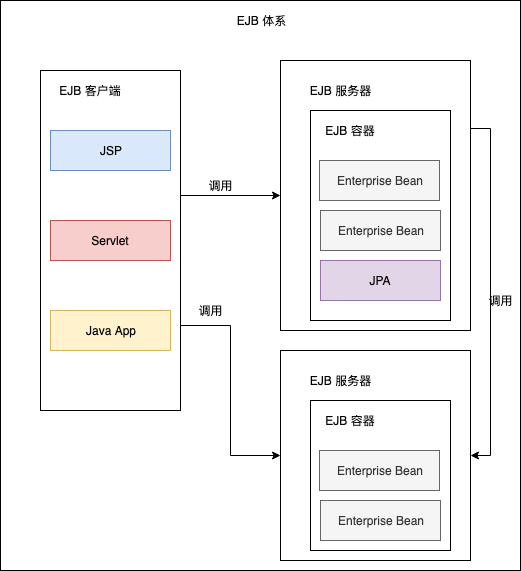
\includegraphics[width=0.7\textwidth]{EJB.png}
    \caption{EJB 框架架构图}
    \label{fig:ejb}
\end{figure}

Spring 框架是目前非常流行的 Java 框架,图\ref{fig:spring} 展示了 Spring 框架的各模块的组织情况。Spring 框架诞生之初就是为了取代类似 EJB 的重量级 Java 框架。Spring 框架通过扩展 POJO(Plain Old Java Object) 提供了一种轻量、方便的编程方式。Spring 框架提供了依赖注入与面向切面编程帮助用户创建低耦合、高内聚以及高可扩展性的应用程序。Spring 框架非常的灵活,用户可以自由选择应用中每一个模块的功能实现,同时也向用户提供了多种看问题的思路。Spring 框架的使用场景非常多,无论是传统网络应用开发还是新兴的微服务系统开发都可以使用 Spring 框架。

\begin{figure}[!ht]
    \centering
    \includegraphics[width=0.7\textwidth]{spring.png}
    \caption{Spring 模块组织图}
    \label{fig:spring}
\end{figure}

根据目前互联网业界的经验以及本次毕业设计的需求来看,EJB 框架过于臃肿复杂,不适合本次应用的开发。本次应用开发将使用 Spring 框架,遵循软件开发过程中的增量模型,即软件开发过程经过若干次迭代,每次迭代都添加部分新功能。Spring 框架的开放性、轻量性与灵活性高度适合互联网应用的开发。因此本次应用设计将基于 Spring 框架进行。

\subsection{数据库技术}

数据库是指长期储存在计算机系统内部的、有组织的、可共享的大量数据的集合,数据库中数据按一定数据模型储存,具有有组织、可共享、冗余度低、独立性高以及可扩展性强等特点。数据库系统使用数据模型来对数据进行抽象、组织与管理。数据模型根据其功能可以分为两大类。第一类是概念数据模型,第二类是逻辑数据模型与物理数据模型。概念数据模型主要用于设计数据库,逻辑数据模型和物理数据模型主要用于数据库的实现。其中,逻辑数据模型根据数据结构的不同还可以分为:层次模型、网状模型、关系模型、面向对象数据模型、对象关系模型以及半结构化数据模型。现在一般使用关系模型作为数据库的了逻辑数据模型。
1970 年 E.F.Codd 提出了关系数据模型。关系数据模型建立在严格的数学基础之上,每一个关系都是一张二维表。关系模型具有许多优点:关系模型的概念比较单一,无论是数据库中抽象出的实体还是这些实体之间的关系都可以用关系表来抽象表示,此外,关系模型中的数据操作时集合操作,其存取路径对于用户来说是隐蔽的,用户在操作时只需指定做什么而不需要告知数据库怎么做,极大地方便了用户使用数据库。

随着互联网的发展,关系型数据库逐渐暴露出了诸多弊端:如关系数据库无法有效地处理大量数据的写入、数据更新时改变表的结构以及简单查询迅速返回结果。为了解决这些弊端,开发者们提出了非关系型数据库。非关系型数据库只用于特定领域,几乎不做复杂运算,它具有易于分散数据、方便提升性能的优点。非关系型数据库根据储存原理的不同又可分为:键值型数据库、文档型数据库和列储存数据库等。键值型数据库原理类似哈希表,一键值对为单元存取数据,其存取速度较快,但存取方式单一,Redis 为键值型数据库最流行的实现。文档型数据库类似一个 JSON 文件,即使不定义表的结构也可像定义了表结构那样使用。MongoDB 是文档型数据库最常用的实现。列储存数据库以列作为储存单元,可以对大量行少数列进行读取,对某一列所有行同时更新,具有高度的可扩展性。HBase 是列储存数据库最常用的实现。

\subsection{视频编码技术}

视频编码技术是对视频进行压缩以更好地进行网络传输的技术。目前最新的视频编码国际标准 - 高效视频编码HEVC,已于2013年由JCT-VC正式颁布,其压缩性能在前一代H.264/AVC的基础上提高了一倍。优秀的视频编码可以有效地在尽可能小地影响画质的基础上对视频进行大幅度地压缩。视频编码技术在本设计中有着重要的作用。

\section{论文的主要工作}

本节介绍了本次毕业设计中的各项具体工作。

首先,本文详细阐述了此次毕业设计使用的各种技术的原理以及整个短视频应用系统架构的设计。在应用系统开发完成后在云服务器平台进行部署与测试。

随后,本文试验了各种数据库优化的方法并对它们进行比较,找出了最适合本系统的数据库解决方案,并与初始状态进行了比较。

最后,本文提出了比较适合短视频应用场景的视频压缩编码方案,对于短视频这种视频长度较小、主要基于移动端以及对画质要求低流畅度要求高等特性做出了对应的优化措施,提高了视频编码时的性能表现。




\section{论文的组织结构}

%论文剩余部分的结构如下:第~~\ref{sec:theory}~~章讲述了本文主要工作的理论框架、模型和算法,第~~\ref{sec:algorithm}~~章详细讲述了项目中各工作的算法及其实现,以及实现过程中使用的协议和参数。第~~\ref{sec:experiment}~~章展示了详细的实验结果,并做了详细地分析和讨论。第~~\ref{sec:conclusion}~~章总结了项目和论文,以及介绍了今后的工作。
        % 理论框架
        \chapter{设计原理}\label{sec:theory}

\section{Spring 框架}

近年来 Spring 框架是 Java Web 框架中经常被使用的,其主要目的是降低应用系统开发时的复杂性。Spring 框架构建基于其核心,Spring 核心模块提供了一个 IoC 容器以及一些举出工具类。Spring AOP 模块位于核心模块之上,这为开发者提供了一系列面向切面编程支持。在 AOP 模块之上是数据访问与事务管理功能\cite{walls2005spring}。下文将详细介绍这三个 Spring 框架的基础功能。

\subsection{Spring 框架的控制反转容器}

控制反转 (Inversion of Control, IoC) 概念来源于依赖倒置原则。依赖倒置原则即高层模块不应该依赖低层模块,二者都应该依赖其抽象;抽象不应该依赖细节;细节应该依赖抽象\cite{gamma1995design}。简单地说,高层模块与低层模块不应该直接产生耦合,高层与低层模块应通过一个接口耦合在一起,即高层模块依赖于该接口,低层模块实现该接口。如图 \ref{fig:beforeAndAfter} 所示,这样对于低层模块的修改就不会对高层模块产生较大的影响同时也减小了系统各模块的耦合。

\begin{figure}[!ht]
\centering
\subfloat[使用 IoC 前]{
	\centering
    %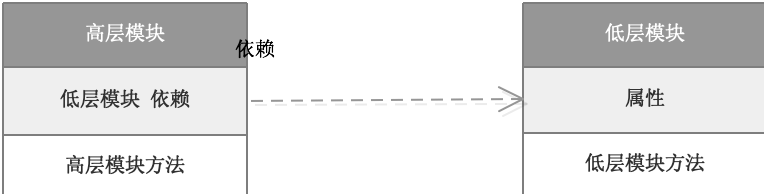
\includegraphics[width=0.5\textwidth]{beIOC.png}}
    \begin{tikzpicture}
        \begin{class}{高层模块}{0,0}
            \attribute{低层模块 : 依赖}
            \operation{高层模块方法 : 返回值}
            % virtual operation
            \end{class}
            
            \begin{class}{低层模块}{7.5,0}
            \attribute{属性}
            \operation{方法}
            % virtual operation
            \end{class}
            
            \aggregation{高层模块}{}{依赖}{低层模块}
    \end{tikzpicture}}\quad
\subfloat[使用 IoC 后]{
    \centering
    %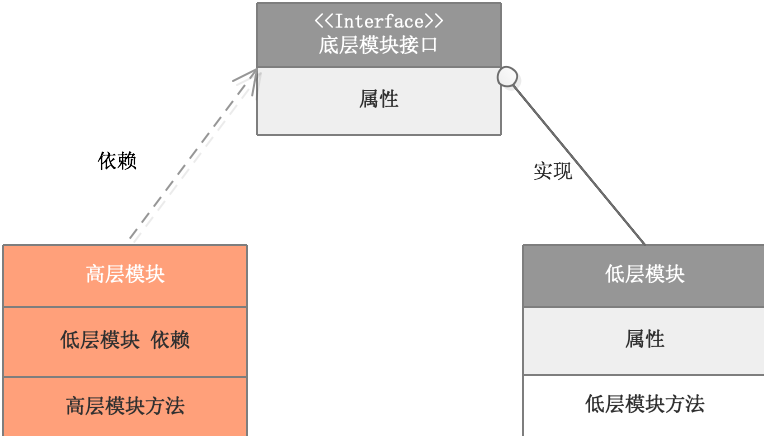
\includegraphics[width=0.5\textwidth]{afIOC.png}
    \begin{tikzpicture}
\begin{interface}{低层模块接口}{0,0}
    \attribute{接口属性}
    \attribute{接口方法} \end{interface}
    
    \begin{class}{高层模块}{-3,-3}
    \attribute{低层模块 : 依赖}
    \operation{高层模块方法 : 返回值}
    % virtual operation
    \end{class}
    
    \begin{class}{低层模块}{3,-3}
    \implement{低层模块接口}
    \attribute{底层模块属性}
    \operation{低层模块方法}
    % virtual operation
    \end{class}
    
    \aggregation{高层模块}{}{依赖}{低层模块接口}
    \end{tikzpicture}
    }
\caption{使用 IoC 前后 UML 图}
\label{fig:beforeAndAfter}
\end{figure}

Spring 的控制反转容器是通过依赖注入 (Dependency Injection, DI) 实现的。如图 \ref{fig:DI} 所示,依赖注入即高层模块在使用低层依赖时,不是自己将低层模块实例化而是向控制反转容器申请一个已创建好的依赖对象\cite{prasanna2009dependency}。这样高层模块与低层模块间的耦合被降低了,对于低层模块的改变对高层模块产生的影响也变小了。同时,由于低层模块由容器创建,我们就可以轻松地实现单例模式等设计模式,进一步简化了开发也提高了系统的性能。通过使用 Spring 框架提供的 IoC 容器,我们可以轻松地使用控制反转构建应用系统。

\begin{figure}[!ht]
    \centering
    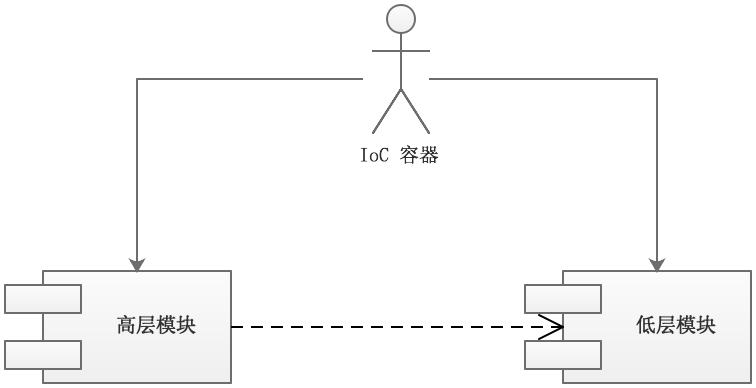
\includegraphics[width=0.6\textwidth]{IoC.png}
    \caption{Spring 依赖注入作用}
    \label{fig:DI}
\end{figure}

\subsection{Spring AOP 框架}

在一个应用系统中存在着一些许多模块公用的功能,如:日志记录、安全检查以及事务功能等。这些公用功能如果处置不当就会造成系统的代码冗余度增加和耦合性上升,例如:要在系统中增加一次日志记录,我们就必须在所有的模块中加入相同的代码,着无疑是非常低效的。对此,我们可以使用面向切面编程 (Aspect Oriented Programming) 来解决这一问题。


\begin{figure}[!ht]
    \centering
    %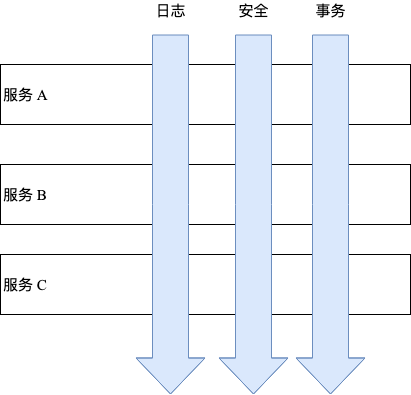
\includegraphics[width=0.4\textwidth]{AOP.png}
    \begin{tikzpicture}
        [Tag/.style={rectangle}]
        \draw (0,0) rectangle (8, 1);
        \draw (0,-1.5) rectangle (8, -0.5);
        \draw (0,-3) rectangle (8, -2);
        \node[anchor=center] (n1) at (3, -1){
\includegraphics[scale=0.6]{arrow}};
        \node[anchor=center] (n2) at (5, -1){
\includegraphics[scale=0.6]{arrow}};
        \node[anchor=center] (n3) at (7, -1){
\includegraphics[scale=0.6]{arrow}};
        \node[Tag] (t1) at (0.6, 0.5) {服务 A};
        \node[Tag] (t2) at (0.6, -1) {服务 B};
        \node[Tag] (t3) at (0.6, -2.5) {服务 C};

        \node[Tag] (t4) at (3, 2.25) {日志};
        \node[Tag] (t5) at (5, 2.25) {安全};
        \node[Tag] (t6) at (7, 2.25) {事务};

    \end{tikzpicture}
    \caption{面向切面编程中的横切关注点}
    \label{fig:AOP}
\end{figure}

如图 \ref{fig:AOP} 所示,面向切面编程可以将系统中的公共功能抽象成为许多称之为横切关注点的功能模块,例如:日志记录功能就是一个横切关注点。系统中需要使用这些公共功能的地方称之为连接点 (Joinpoint)\cite{walls2005spring}。在系统运行时面向切面编程框架会将横切关注点织入连接点中,这样系统就可以使用所有的公共功能,减少了系统的冗余代码与耦合性。

Spring 框架中的面向切面编程功能由动态代理实现,源于设计模式中的代理模式。如图 \ref{fig:Proxy} 所示,代理模式的作用是为隔离被代理对象,使用代理提供功能调用\cite{gamma1995design}。代理处于访问者与被访问者之间,隔离两者的直接交互。在代理将访问者的访问请求传递给被访问者时,代理可以添加一部分额外的功能,如安全检测。因此,代理模式可以有效地增强系统的灵活性与安全性。动态代理的实现还要依靠 Java 提供的反射功能。反射功能允许我们在 Java 程序的运行期间动态载入类、创建对象以及生成代理。通过实现代理模式、使用反射机制,我们就可以创建出动态代理系统,实现面向接口编程\cite{walls2005spring,walls2016spring}。

\begin{figure}[!ht]
    \centering
    %\includegraphics[width=0.6\textwidth]{Proxy.png}
    \begin{tikzpicture}
\begin{abstractclass}{Subject}{0 ,1}
    \attribute{}
    \operation{+ request()}
    \end{abstractclass}
    
    \begin{class}{Proxy}{-4,-3}
    \inherit{Subject}
    \attribute{- realSubject : RealSubject}
    \operation{+ preRequest()}
    \operation{+ request()}
    \operation{+ postRequest()}
    % virtual operation
    \end{class}
    
    \begin{class}{RealSubject}{4,-3}
    \inherit{Subject}
    \attribute{}
    \operation{+ request()}
    % virtual operation
    \end{class}
    
    \begin{class}{Client}{-6,1}
    \attribute{}
    \operation{+ request()}
    % virtual operation
    \end{class}
    
    \unidirectionalAssociation{Proxy}{realSubject}{}{RealSubject}
    
    \draw[umlcd style dashed line, ->] (Client) --node[above, sloped, black]{} (Proxy);
    
    \end{tikzpicture}
    \caption{代理模式 UML 图}
    \label{fig:Proxy}
\end{figure}

Spring AOP 的设计遵循了 8/2 原则,即通过 20\% 的代码实现 AOP
 框架 80\% 的功能。因此Spring AOP 支持的 AOP 功能是不完全的,例如 Spring AOP 不支持属性级别的拦截等。系统运行时,我们在系统中定义所有的切面、连接点都会被 Spring AOP 拼装起来,这个操作被称为织入\cite{spring2019}。织入时,Spring 会自动生成切面的代理包装类,通过代理包装类将切面织入代码中。Spring AOP 框架为我们提供了 AOP 的大部分功能,同时我们也可以整合使用 AspectJ 等框架来获取 Spring AOP 不支持的功能。
 
 \subsection{Spring 事务管理功能}
 
 事务管理的作用是保证应用系统在操作数据库时不会对数据的正确性产生破坏,具体的事务定义将在下文介绍。在 Spring 框架中,我们通常使用声明式的方式使用事务,事务也是一个常用的 AOP 中的横切关注点。通常情况下使用事务,我们需在每次访问数据库前声明事务开始,在事务正常结束后进行结束事务操作,在事务异常结束后进行事务的回滚。Spring 框架使用 AOP 来处理事务,通过在运行时将事务代码织入应用中来简化开发\cite{spring2019,walls2005spring}。
 
 我们在需要使用事务的地方使用 @Transactional\cite{spring2019} 注解即可开启声明式事务功能。我们可以在其中设置一些事物属性。事务属性主要包括:隔离级别、传播行为、回滚规则、是否只读以及超时时间等。通过注解使用声明式事务对于简化数据访问层的开发具有较大的意义\cite{walls2016spring}。


\section{数据库的原理与设计}

本次设计采用 MySQL 作为系统主数据库、Redis 作为缓存数据库。


\subsection{关系型数据库}
支持关系模型的数据库系统为关系型数据库系统。关系模型主要数据结构为关系{codd1970relational}。关系中的域是一组具有相同数据类型的值的集合。一个关系可以由多个域的笛卡尔积表示。如一个班中所有学生的年龄的集合就是一个域\cite{王珊2006数据库系统概论}。

笛卡尔积是一种域上的集合运算,其定义为:
\begin{equation}
\label{eq:Descartes}
D_1 \times D_2 \times \cdots \times D_n = {(d_1, d_2, \cdots, d_n) | d_i \in D_i, i=1, 2, \cdots, n}
\end{equation}
其中,每一个元素 $(d_1, d_2, \cdots, d_n)$ 为一个元组。笛卡尔积可以表示一个二维表,表中的一行对应笛卡尔积中的一个元组。$D_1 \times D_2 \times \cdots \times D_n$ 的子集为在域 $D_1, D_2, \cdots, D_n$ 上的关系\cite{codd1970relational}。

每一个关系中都存在一些特殊的属性。若关系中某一属性组可以唯一标志该元组,而其任意子集均无此性质,则该属性组为这个关系的候选码。任意包含在至少一个候选码中的属性为主属性,不包含在所有候选码中的属性为非主属性。在任意关系表中不可能存在具有相同候选码的两个或多个元组\cite{codd1970relational,王珊2006数据库系统概论}。

关系模式可以表示为 $R(U, D, DOM, F)$,其中 $R$ 为关系名,$U$ 为属性名的集合,$D$ 为域的集合,$DOM$ 为属性与域的映射,$F$ 为属性间的依赖关系。关系模式中主要包含关系中有哪些属性、关系中有哪些域以及域与属性的映射关系。

关系数据模型中具有关系的操作。集合操作有:并 (union, $\cup$ ) 、差 (except, $-$ ) 、交 (intersection, $\cap$ ) 、除 (divide, $\div$ ) 和笛卡尔积 (Descartes Product, $\times$ )。关系专用操作包括:选择 (select, $\sigma$) 、投影 (project, $\Pi$) 以及连接 (join, $\Join $)。其中,选择、投影、并、差、笛卡尔积是基本操作\cite{ullman1984principles}。

\begin{figure}[!ht]
    \centering
    %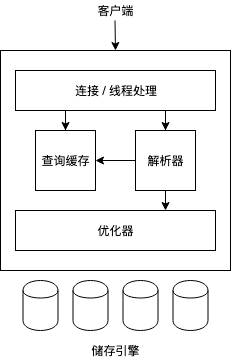
\includegraphics[width=0.4\textwidth]{db1.png}
    \begin{tikzpicture}
[Tag/.style={rectangle},
Block/.style={rectangle,draw=black,fill=white,very thick, minimum width=65mm, minimum height=10mm},
Block2/.style={rectangle,draw=black,fill=white,very thick, minimum width=20mm, minimum height=20mm}]

\node[cylinder,draw=black,thick,aspect=0.7,minimum height=1.7cm,minimum width=1.5cm,shape border rotate=90,cylinder uses custom fill, cylinder body fill=red!30,cylinder end fill=red!10] (A) at (0,0) {引擎};

\node[cylinder,draw=black,thick,aspect=0.7,minimum height=1.7cm,minimum width=1.5cm,shape border rotate=90,cylinder uses custom fill, cylinder body fill=red!30,cylinder end fill=red!10] (A) at (1.75, 0) {引擎};

\node[cylinder,draw=black,thick,aspect=0.7,minimum height=1.7cm,minimum width=1.5cm,shape border rotate=90,cylinder uses custom fill, cylinder body fill=red!30,cylinder end fill=red!10] (A) at (3.5, 0) {引擎};

\node[cylinder,draw=black,thick,aspect=0.7,minimum height=1.7cm,minimum width=1.5cm,shape border rotate=90,cylinder uses custom fill, cylinder body fill=red!30,cylinder end fill=red!10] (A) at (5.25, 0) {引擎};

\draw (-1,1.2) rectangle (6.2, 7.75);

\node[Block] (b1) at (2.6, 2.25) {优化器};
\node[Block2] (b2) at (1, 4.5) {查询缓存};
\node[Block2] (b3) at (4.2, 4.5) {解析器};

\node[Block] (b4) at (2.6, 6.75) {连接/线程处理器};

\node[Tag] (t1) at (2.6, 8.75) {客户端};

\node[Tag] (t2) at (2.6, 7.65) {};

\draw[-{Stealth[length=3mm, round]}] (4.2,3.5)--(4.2,2.75);
\draw[-{Stealth[length=3mm, round]}] (3.2,4.5)--(2,4.5);
\draw[-{Stealth[length=3mm, round]}] (4.2,6.25)--(4.2,5.5);
\draw[-{Stealth[length=3mm, round]}] (1,6.25)--(1,5.5);
\draw[-{Stealth[length=3mm, round]}] (2.6,8.5)--(2.6,7.75);
    \end{tikzpicture}
    \caption{MySQL 架构分析图}
    \label{fig:db1}
\end{figure}


\subsection{数据库事务}

数据库事务是用户定义的一个数据库操作序列,是不可分割的工作单位。事务具有四个特征,分别是原子性:一个事务是不可分割的,事务内所有操作的状态必须一致;一致性:事务的作用必须使数据库从一个一致状态变为另一个一致状态;隔离性:多个事务的执行互不干扰;持续性:事务对数据库的修改是永久的。数据库事务是在并发条件下保证数据库数据正确的总要条件。

\subsection{MySQL 原理}
MySQL 是一个开源的关系型数据库管理系统。MySQL 非常的灵活,可以适应多种运行场景,例如:MySQL 既可以嵌入在程序中运行也可以支持数据仓库、在线处理系统等应用\cite{姜承尧2011mysql}。MySQL 主要由两部分组成:客户端与服务端。客户端的作用是向数据库系统发出命令并获取命令执行结果。服务端就是数据库系统本身,负责处理查询语句、执行查询并将查询结果返回客户端。

MySQL 是一个层次化系统,如图 \ref{fig:db1} 所示,主要包括 SQL 接口、查询 MySQL 解析器、MySQL 查询优化器以及查询执行引擎、缓冲/缓存机制和一个插件式的储存引擎。第二层服务是 MySQL 的核心,第三层则包括了储存引擎,它负责数据库中数据的储存与提取。我们可以根据需要选择不同功能的查询引擎\cite{schwartz2012high}。


MySQL 默认的库表结构与查询优化是不能有效地满足应用性能需求的,为此,我们需对 MySQL 的运行过程进行合理地优化。为了实现 MySQL 的高性能运行,我们需要对 MySQL 进行查询优化、索引优化以及库表结构优化。库表结构优化指为数据库选取合适的数据类型、合理使用 MySQL 特性以及使用缓存等操作。索引优化指在数据库表中的某些列上添加正确的索引以加快查询速度。查询优化指合理设置查询方式,使得查询产生的中间结果最少、查询过程合理使用索引及物理结构,使得查询速度加快。

\subsection{数据库设计原理}

本项目中采用基于 E-R (Entity - Relation, 实体 - 关系) 模型的设计方法进行设计。如图 \ref{fig:db2} 所示,数据库设计主要分为六个阶段:需求分析、概念设计、逻辑设计、物理设计、数据库实施以及数据库运行与维护\cite{王珊2006数据库系统概论}。

\begin{figure}[!ht]
    \centering
    %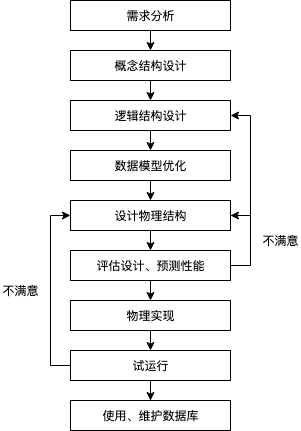
\includegraphics[width=0.4\textwidth]{db2.png}
    \begin{tikzpicture}
[Tag/.style={rectangle},
White/.style={rectangle,draw=black,fill=white,very thick, minimum width=65mm, minimum height=10mm},
White2/.style={rectangle,draw=black,fill=white,very thick, minimum width=20mm, minimum height=20mm},]

\node[White] (b1) at (0, 0) {使用/维护数据库};
\node[White] (b2) at (0, 1.75) {试运行};
\node[White] (b3) at (0, 3.5) {物理实现};
\node[White] (b4) at (0, 5.25) {评估设计、预测性能};
\node[White] (b5) at (0, 7) {物理结构设计};
\node[White] (b6) at (0, 8.75) {数据模型优化};
\node[White] (b7) at (0, 10.5) {逻辑结构设计};
\node[White] (b8) at (0, 12.25) {概念结构设计};
\node[White] (b9) at (0, 14) {需求分析};

\draw[-{Stealth[length=3mm, round]}] (b9)--(b8);
\draw[-{Stealth[length=3mm, round]}] (b8)--(b7);
\draw[-{Stealth[length=3mm, round]}] (b7)--(b6);
\draw[-{Stealth[length=3mm, round]}] (b6)--(b5);
\draw[-{Stealth[length=3mm, round]}] (b5)--(b4);
\draw[-{Stealth[length=3mm, round]}] (b4)--(b3);
\draw[-{Stealth[length=3mm, round]}] (b3)--(b2);
\draw[-{Stealth[length=3mm, round]}] (b2)--(b1);

\draw[-{Stealth[length=3mm, round]}] (3.25, 5.25)--(4, 5.25)--(4, 10.5)--(3.25,10.5);

\draw[-{Stealth[length=3mm, round]}] (3.25, 5.25)--(4, 5.25)--(4, 7)--(3.25,7);

\draw[-{Stealth[length=3mm, round]}] (-3.25, 1.75)--(-4, 1.75)--(-4, 7)--(-3.25,7);

\node[Tag] (t1) at (4.75, 5.5) {不满意};
\node[Tag] (t2) at (-5, 2) {不满意};

    \end{tikzpicture}
    \caption{数据库设计流程图}
    \label{fig:db2}
\end{figure}

设计数据库时,首先必须分析设计需求,需求分析过程是整个设计的基础。随后,在需求分析的基础上开始概念结构设计,产出数据库概念结构。完成概念设计后,进行逻辑结构设计,将概念模型转换为数据库管理系统支持的逻辑模型,并进行优化。随后进行物理结构设计,即为设计好的逻辑结构选取最合适的物理结构。物理结构设计完成后,使用数据库语言建立相应的数据库、调试并进行数据入库。完成上述过程后,数据库即可开始运行,在运行时需根据实际情况作出调整与适当地维护\cite{wiederhold1983database}。

\section{微信小程序}

微信小程序的开发要基于微信小程序开发框架。微信小程序开发框架将微信小程序分为逻辑层与视图层。逻辑层由 JavaScript 语言编写,负责处理小程序的逻辑操作与后端交互。视图层由 wxml 和 wxss 编写,负责渲染出开发者想要的页面。微信小程序的开发以页面为单位,每个页面都是一个独立的单位。开发时,首先要在配置文件中注册所有的页面,随后便可以逐个页面进行开发。


\section{视频编码}

在网络上进行传输的视频必须经过编码与压缩。网络传输的高清视频分辨率通常为 1920 $\times$ 1080,帧率为 30 帧,这样的视频如果不进行编码与压缩,一秒钟的视频产生文件大小为 177M 字节,移动网络大部分情况都不能以如此高的速率加载视频。因此要对视频进行编码与压缩,以某种方式压缩视频的算法称为视频编码。

目前主流的视频编码有 h.264\cite{richardson2004h} 和 h.265\cite{万帅2014新一代高效视频编码} 编码。h.264 编码比较成熟与稳定,目前所有的移动设备均能流畅解码播放,兼容性较好同时其编码器效率较高,编码速度较快,同时 h.264 编码的缺陷在于压缩率不如 h.265 编码。h.265 编码是最新的视频编码,h.265 编码的压缩率较高,h.265 编码视频只需使用 h.264 编码视频码率的一般即可达到同样的画质效果。h.265 编码的缺陷在于兼容性不如 h.264 编码,且编解码所需时间较长。

视频编码常用压缩算法主要有帧间压缩和帧内压缩。帧内压缩就是将视频的每一帧图像都进行有损压缩,如 Jpeg 压缩。其基本原理为应用人眼对亮度敏感同时对色彩不敏感的特性,尽可能保留图像的亮度信息,大幅压缩图像的色彩信息,以减小图像的大小。帧间压缩的原理是不保存视频所有的帧,只保留视频的关键帧以及两个关键帧之间像素的变化情况,具体原理如图 \ref{fig:video1} 所示。帧间压缩通常采用帧间预测编码来实现\cite{richardson2004h}。

\begin{figure}[!ht]
    \centering
    %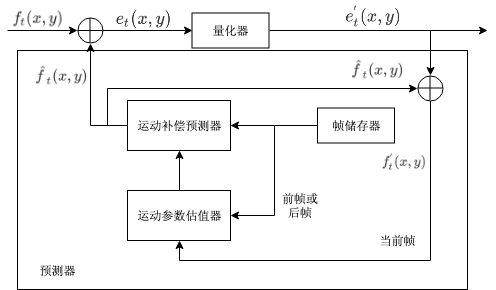
\includegraphics[width=0.6\textwidth]{video1.png}
\begin{tikzpicture}
    [Tag/.style={rectangle},
White/.style={rectangle,draw=black,fill=white,very thick, minimum width=20mm, minimum height=10mm}]

\node[draw,circle,minimum width=0.5cm,add={}{}{}{}] (circle) at (0,0) {};
\node[Tag] (t1) at (-2, 0) {};
\node[Tag] (tn) at (10, 0) {};
\node[Tag] (t2) at (-1, 0.25) {$f_{t}(x,y)$};

\node[Tag] (t3) at (1.5, 0.25) {$e_{t}(x,y)$};

\node[White] (w1) at (4, 0) {量化器};

\node[White] (w2) at (2, -3) {运动补偿预测器};

\node[Tag] (t4) at (-0.6, -1.5) {$\hat{f}_{t}(x,y)$};

\node[White] (w3) at (6, -3) {帧储存器};
\node[draw,circle,minimum width=0.5cm,add={}{}{}{}] (circle2) at (8,-2) {};

\node[Tag] (t5) at (4, -1.7) {$\hat{f}_{t}(x,y)$};

\node[White] (w4) at (2, -5) {运动参数估计器};

\node[Tag] (t5) at (5, -4.5) {前帧或后帧};
\node[Tag] (t6) at (7, 0.25) {$e^{'}_{t}(x,y)$};

\node[Tag] (t6) at (7.3, -4) {$f^{'}_{t}(x,y)$};
\node[Tag] (t6) at (7.3, -5.7) {当前帧};

\draw[-{Stealth[length=3mm, round]}] (t1)--(circle); 
\draw[-{Stealth[length=3mm, round]}] (circle)--(w1); 
\draw[-{Stealth[length=3mm, round]}] (w2)--(0, -3)--(circle); 
\draw[-{Stealth[length=3mm, round]}] (w3)--(w2); 
\draw[-{Stealth[length=3mm, round]}] (w2)--(0.4, -3)--(0.4, -2)--(circle2);
\draw[-{Stealth[length=3mm, round]}] (w4)--(w2);
\draw[-{Stealth[length=3mm, round]}] (w3)--(4,-3)--(4, -5)--(w4);
\draw[-{Stealth[length=3mm, round]}] (w1)--(tn);
\draw[-{Stealth[length=3mm, round]}] (w1)--(8, 0)--(circle2);
\draw[-{Stealth[length=3mm, round]}] (circle2)--(8, -6)--(2, -6)--(w4);
\end{tikzpicture}
    \caption{单向预测帧间编码}
    \label{fig:video1}
\end{figure}

帧间预测编码的基础是单向预测算法。单向预测算法通常将视频整个画面划分为若干块,以块为单位分配运动矢量\cite{毕厚杰2005新一代视频压缩编码标准}。如图 \ref{fig:video1} 所示,把当前帧 $f_{t}^{'})(x,y) $ 与前一帧 $f_{t-1}(x,y)$ 输入运动参数估计器中,运算后得到运动矢量,运动矢量输入补偿器得到预测图像 $\hat{f}_{t}(x,y)$。利用上一帧图像与运动矢量得到当前图像的算法称为单向预测算法:
\begin{equation}
\label{eq:forward_pre}
\hat{f}_{t}(x,y) = f_{t}(x+i, y+i)
\end{equation}
其中,$(i, j)$ 为运动矢量。目前通常采用基于单向预测算法的双向预测算法,即同时利用前一帧图像与后一帧图像进行预测:
\begin{equation}
\label{eq:forward_back_pre}
\hat{f}_{t}(x,y) = \alpha_{t-1}f_{t}(x+i, y+i) + \alpha_{t+1}f_{t}(x+i^{'}, y+i^{'})
\end{equation}
双向预测算法不可用于实时视频当中,只能用于实现录制好播放的视频中。

h.264 编码的视频中主要包含三种类型的帧:I 帧、P 帧以及 B 帧,表示运动补偿形式的不同。其中,I 帧为帧内编码帧也叫关键帧,保留完整的图像信息,对于视频进度条跳转有很大帮助。P 帧为帧间预测编码帧,且只能前向预测,它只参考前面最靠近它的I帧或者P帧。B 帧也是帧间预测编码帧, 它可以双向预测。每一个 I 帧以及它与下一个 I 帧之间所有的 P 帧与 B 帧称为一个 GOP 序列。B 帧的压缩率最大,解码的性能也最差,大量使用 B 帧可以节省空间放入更多的 I 帧,相同码率下画质会更好。因此在编码时要合理地设置 GOP 序列大小以及 B 帧的使用\cite{richardson2004h}。

\subsection{数据库与视频编码优化评价标准}
\subsubsection{数据库优化评价标准}
MySQL 主要测试指标有:吞吐量、响应时间、并发性以及可扩展性。吞吐量是指数据库每秒处理的事务的数量。数据吞吐量对于有大量用户同时访问的应用系统来说十分重要,直接决定系统的承载能力,常用测试单位为每秒事务数 (TPS)。响应时间指数据库系统完成一个任务所需要的平均时间,响应时间过长会造成数据库并发瓶颈,通常使用百分比响应时间 (percentile response time, PRT) 作为单位。并发性指数据库系统允许多少请求同时访问,通常测试并发数增加与吞吐量变化的关系。可扩展性指数据库系统在数据量增大时,能否增强其处理能力的特性\cite{schwartz2012high}。

\subsubsection{视频编码评价标准}

视频编码的评价标准主要有编码后视频的体积、编码时间以及某一码率下视频画质。编码后视频体积表示了当前编码器设置的压缩率好坏。编码所用时间表示编码一段短视频耗费时间,视频编码时间不能过长。视频画质表示码率一定时不同编码方案的画质好坏,采用峰值信噪比 ($PSNR$) 作为单位\cite{毕厚杰2005新一代视频压缩编码标准},计算方法:
\begin{equation}
\label{eq:forward_back_pre}
PSNR_{dB} = \frac{10log_{10}(2^{n} - 1)^{2}}{MSE}
\end{equation}
其中 $MSE$ 为原始视频与编码后视频图像之间的均方误差,n 为每个像素的比特数。

\section{本章小结}
本章讲述了本文主要使用的技术框架与理论,包括 Spring 框架、数据库设计与优化技术以及视频压制优化技术等,这些框架与技术有着重要的作用。下一章将叙述应用系统具体实现方案与对应的优化操作。








        % 算法实现
        \chapter{项目内容及优化实现}\label{sec:algorithm}

\section{数据库的设计}
 
\subsection{需求分析}
设计数据库首先要进行需求分析\cite{gamma1995design}。本系统需要数据库来管理与储存用户信息、视频信息、视频的评论信息用户以及用户与视频的各种关系。用户信息包含用户的系统内唯一编号、用户名、密码、注册时间、用户头像以及用户各项统计信息等内容。视频信息包括视频名称、视频文件存放位置、视频作者、视频相关统计信息等内容。评论信息包含评论人、评论内容、评论种类、评论视频等内容。用户与视频关系包含关系类型、用户编号与视频编号等内容。

为了需求分析的简便,我们先将用户与视频所有的信息放入一张表中,随后我们要进行关系的规范化。

\subsection{关系规范化}

经过初步地需求分析后,我们得到了一个初步地数据库模型,但这个模型仅仅遵循了关系数据库理论的第一范式\cite{codd1972further},即所有的属性均为原子属性。仅遵循第一范式的模型有插入异常、删除异常以及修改复杂等缺点。以此模型中的用户表为例。当一个用户没有任何视频时无法将该用户插入,导致更新异常。当一个用户信息需变更时需改变所有包含用户信息的元组,导致修改复杂。当用户删除所有视频时会导致用户信息被一同删除,导致删除异常。

为了解决这些问题,我们需要使数据库符合第二范式\cite{codd1972further},即关系遵循第一范式,且关系中所有的非主属性都完全函数依赖于任何候选码。为了使关系遵循第二范式,我们要对其进行规范化,即将一个大的关系拆分为两个或多个小的关系。我们将用户表拆分为用户信息表和视频信息表,两个表的函数依赖关系在拆分后由外健保留,关系拆分后 E-R 图 (省略实体的属性) 如图 \ref{fig:ER2} 所示 。

\begin{figure}[!ht]
    \centering
    %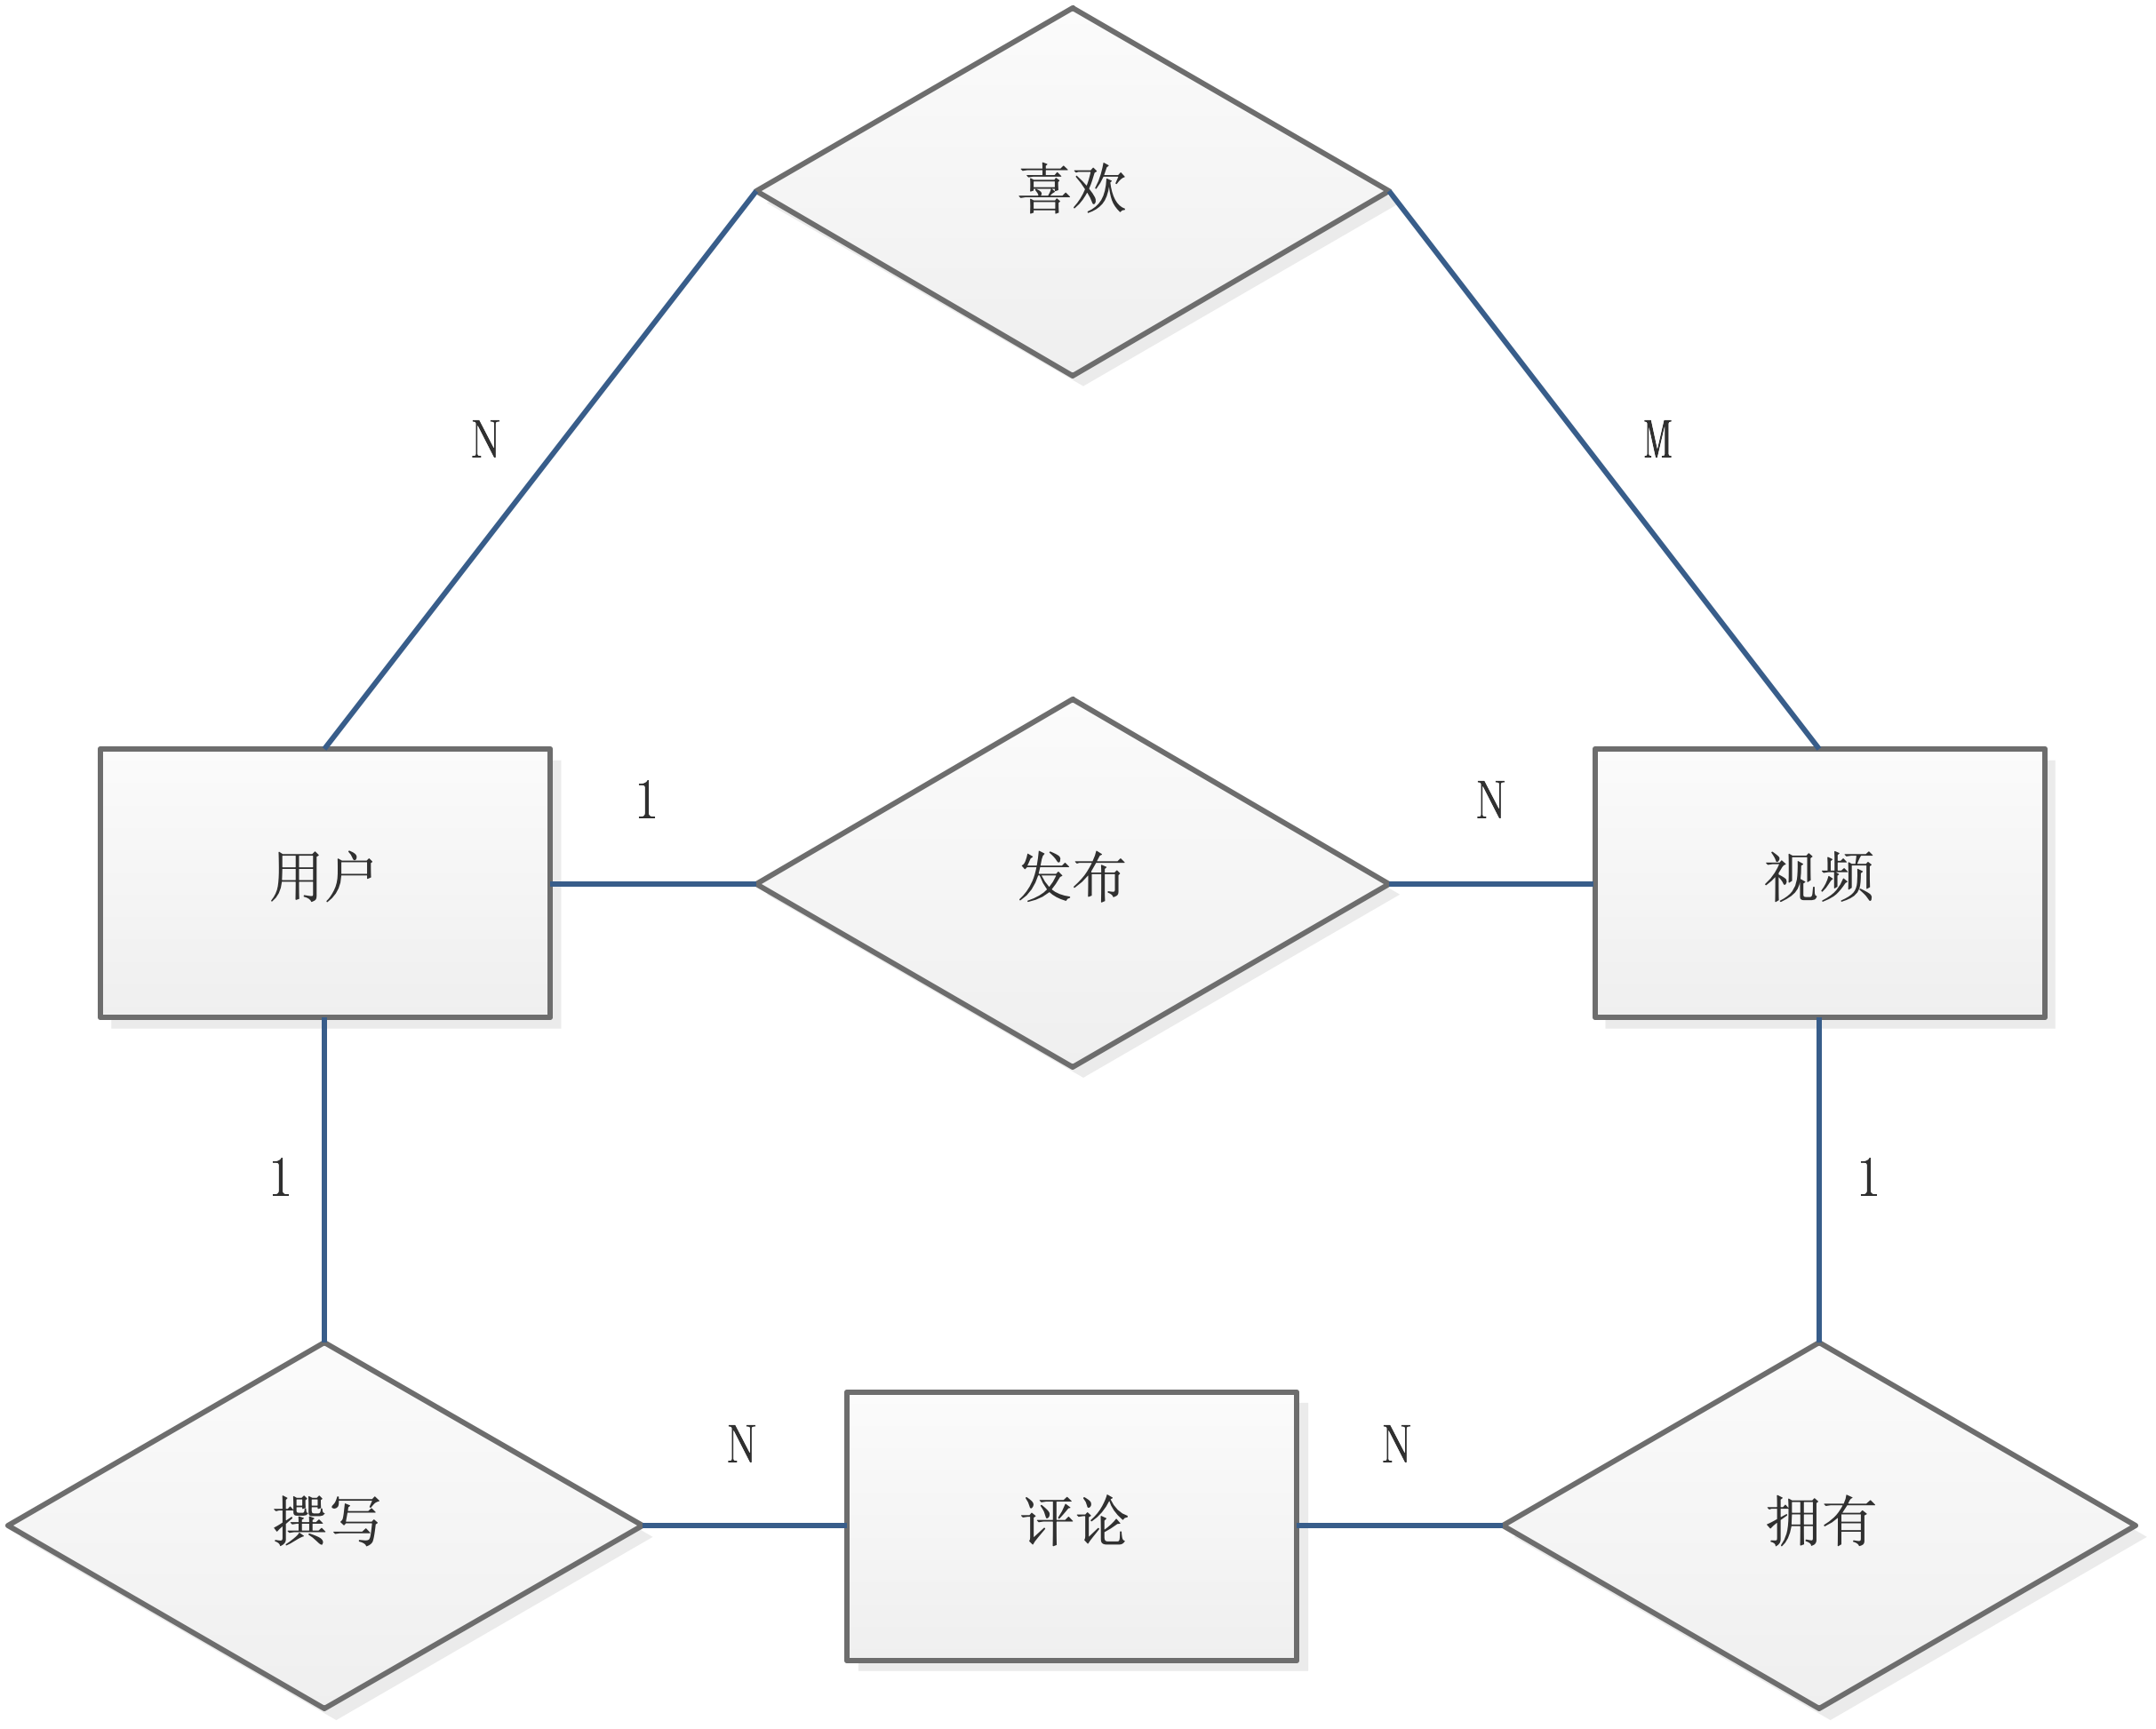
\includegraphics[width=0.6\textwidth]{dbs2.png}
    \begin{tikzpicture}[auto,node distance=1.5cm]
        \node[entity] (user) at (0, 0) {用户};
	\node[entity] (video) at (5, 0) {视频};
	\node[entity] (comment) at (2.5, -2.5) {评论};
	\node[relationship] (publish) at (2.5, 0) {发布};
	\node[relationship] (love) at (2.5, 2.5) {喜欢};
	\node[relationship] (write) at (0, -2.5) {撰写};
	\node[relationship] (have) at (5, -2.5) {拥有};
	
	\path (publish) edge node {1} (user)
    edge node {n}	(video);
	
	\path (love) edge node {n} (user)
    edge node {m}	(video);
	
	\path (write) edge node {1} (user)
    edge node {n}	(comment);
	
	\path (have) edge node {1} (video)
    edge node {n}	(comment);
    \end{tikzpicture}
    \caption{规范化后数据库 E-R 图}
    \label{fig:ER2}
\end{figure}

经过关系分解后,用户表与视频表中即不存在关于主属性的传递函数依赖,也不存在非主属性决定子,所以分解后整个关系达到了 BCNF\cite{bernstein1976synthesizing},解决了之前可能出现的问题。

\subsection{数据库逻辑结构设计}

完成数据库的概念结构 (E-R 模型) 后开始设计数据库逻辑结构\cite{gamma1995design}。这里我采用将 E-R 模型转换为关系模型的方法设计数据库逻辑结构。首先以 E-R 模型中各个实体为基础创建关系模式,然后创建实体间的联系。用户与视频间的发布联系是一个一对多联系,将其与 n 端对应的模式即视频关系模式合并。用户与视频间的关系为多对多关系,需单独设置一个关系模式储存。用户与评论以及视频与评论间的联系是一个多元联系,需单独设置一个关系模式\cite{王珊2006数据库系统概论}储存。

本系统使用的关系模式为:用户模式(\uline{用户编号},用户名,用户密码,用户头像,用户统计信息)、视频模式(\uline{视频编号},视频名称,视频位置,视频作者,视频统计信息)、用户与视频间关系模式(\uline{用户编号},\uline{视频编号},关系类型)、用户、视频与评论关系(\uline{评论编号},用户编号,视频编号,评论类型,评论内容)。

\subsection{数据库物理结构设计与实施}

数据库物理结构由 MySQL 数据库管理系统默认生成,将上述关系模式转换为对应的结构化查询语句,并在 MySQL 中创建出相应的数据库表。完成数据库的实施之后,数据库设计完成。



\section{系统代码编写}

\subsection{系统整体设计}
本系统采用层次化结构进行开发,即将系统的功能由底至顶划分为若干层次,各层之间只能逐层单向调用,只能高级层次模块调用低级层次模块,系统各层次之间只提供相应接口,同时将具体实现屏蔽,这样增大了系统各模块内部的内聚度,减小了模块之间的耦合度,有利于系统开发。

根据短视频系统的功能要求,本系统被划分为公用功能层、数据访问层、服务层以及应用接口层。如图 \ref{figs:soft1} 所示,公用功能层是整个系统的最底层,含有许多供上层模块使用的静态依赖。数据访问层包含两部分一部分是数据访问对象模块,负责操作数据库;另一部分是实体对象模块负责保存数据库返回的结构。服务层依赖于数据访问层,它负责接收应用接口层发送的请求,做与数据相关的前期处理,封装相应的数据访问操作,并将结果进行处理后返回应用接口层。应用接口层接收用户请求,并作出权限判断等于前端有关的处理后将请求转发给服务层,接收结果后封装成响应结构返回给用户。后端开发完毕后,即可按照系统功能划分开发相应的小程序页面,并与后端系统进行交互。

\begin{figure}[!ht]
    \centering
    %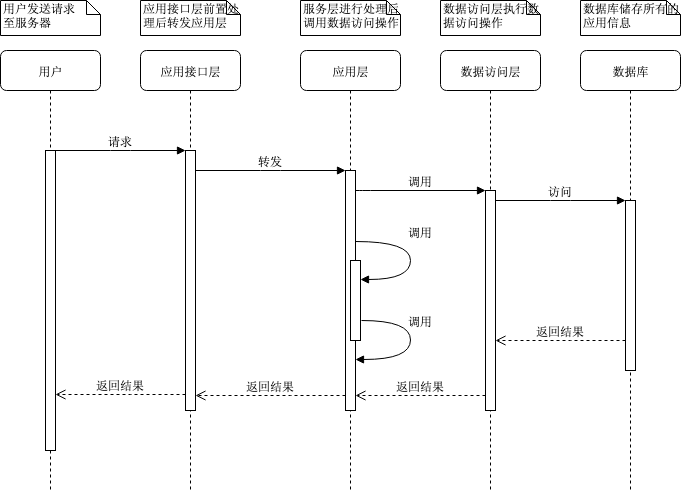
\includegraphics[width=0.8\textwidth]{soft1.png}
    \begin {sequencediagram}
\newthread{User}{用户}
\newinst[1]{api}{应用接口层}
\newinst[1]{service}{服务层}
\newinst[1]{dao}{数据访问层}
\newinst[1]{db}{数据库}

\begin{call}{User}{发送请求}{api}{返回请求数据}
    \begin{call}{api}{转发操作}{service}{返回操作结果}
        \begin{call}{service}{调用}{service}{结果}
        \end{call}
        \begin{call}{service}{调用}{dao}{返回结果}
            \begin{call}{dao}{查询数据}{db}{返回数据}
            \end{call}
        \end{call}
    \end{call}
\end{call}

\end{sequencediagram}
    \caption{短视频系统时序图}
    \label{figs:soft1}
\end{figure}

\subsection{系统具体实现}
本系统的应用接口层由 SpringMVC 实现、服务层由 Spring IoC 与 Spring AOP 实现、数据访问层基于 MyBatis 框架与 Spring AOP。

应用接口层包含了系统内所有的应用编程接口 (Application Programming Interface, API)。这些 API 主要可以分为三组:与用户相关的 API、与视频管理相关的 API以及处理用户与视频关系的 API。这些 API 均基于 SpringMVC 的注解式 API 声明。服务层包含了系统最主要的功能实现,主要使用 Spring IoC 提供的依赖注入功能获取数据访问依赖。数据访问层基于 MyBatis 框架,编写相应的实体类和访问接口后即可有 MyBatis 负责相应数据的读取与封装,并且使用 Spring AOP 实现对数据库事务的支持。



\section{短视频压缩编码初步实现实现}

短视频的压制与背景音乐合成由 FFmpeg\cite{ffmpeg2019} 实现。FFmpeg 是一组音视频处理工具的集合。根据短视频应用的特性,我初步地将视频分辨率设为 1920 $\times$ 1080,帧率设置为 30 帧,码率采用 2 Mbps,编码采用 h.264 编码,封装格式采用 Mpeg4,兼容性较好,该压制属性可以保证视频中等清晰。

%\begin{lstlisting}
%ffmpeg -i input.MOV -vcodec h264 -profile:v high -level 5.1 -s 1920x1080 -preset slow -b:v 4M -maxrate 8M -bufsize 4M -r 29.97 output.mp4
%\end{lstlisting}



\section{数据库性能优化}

MySQL 优化是指通过各种方式调整 MySQL 或服务器以提升 MySQL 数据库具体性能表现的过程。数据库优化主要可以分为架构优化、参数优化和 SQL 优化。架构优化指对整个系统架构进行分析重构与优化,通常获得结果最好,但最复杂。参数优化指调整操作系统与数据库的参数设置来进行优化的方法,其效果通过基准测试体现。SQL 优化指针对具体数据库表与查询语句进行工程上的调整,效果通过压力测试体现。本文只关注参数优化和性能优化对数据库的性能提升效果。

\subsection{参数优化}

数据库的参数优化\cite{schwartz2012high}是通过调节操作系统与数据库的参数设置来实现的。参数优化的过程中要遵循的原则有重视数据库记录日志、多次进行数据库瓶颈分析以及注意实现数据库读写的平衡。

对于一个事务序列来说最重要的是其能否成功执行。而事务能否成功执行的关键在于其日志文件能否成功落盘保存。因此日志文件对于事务序列方面的优化起着至关重要的作用。其次,我们需要通过查看数据库的监控信息查找数据库的瓶颈并做针对性优化。最后,为了数据库有一个良好的整体性能,我们需要根据我们的系统实际情况对数据库读写性能进行平衡。

在本系统中,我们可以调节数据库内存缓存的大小,以减小磁盘 I/O 操作,以达到更好地性能。随后,我们可以根据数据库的日志文件进行优化,减少数据库日志文件的刷新,以获得更好地性能。最后可以根据监控数据进行优化,观察监控数据中数据库对各项系统资源的占用情况,若 CPU 是系统瓶颈则可以增大线程池以减小线程创建次数。若磁盘称为瓶颈则可以降低并发以获得更好地性能。

本系统选择将 MySQL 数据库的 InnoDB\cite{姜承尧2011mysql} 储存引擎的 innodb\_buffer\_pool\_size 参数设置为 70\% 内存大小,以达到较好的磁盘性能。然后,将 innodb\_buffer\_pool\_size 属性设置为 4G,减小 MySQL 日志产生数量,提高性能。将 innodb\_flush\_logs\_at\_trx\_commit 属性设置为 0,这样做虽然会减小一定的稳定性但会带来较大的性能提升,本系统不需要太高的一致性,所以可以对其进行更改。最后设置合适的允许连接数、开启慢日志查询以及设置合理地缓存命中率对数据库性能均有明显提升。


\subsection{SQL 优化}

数据库的 SQL 优化主要包括为数据库表选取合适的数据类型、选用合适的索引以及优化查询过程等方面。

\subsubsection{适当的数据类型}

数据类型优化原则有尽可能使用较小的数据类型、使用较简单地数据类型以及避免使用 null。较小的数据类型通常处理起来比较快,同时它们占有较小的磁盘空间、内存以及 CPU 缓存,可以在更短的时钟周期内处理。简单数据类型或数据库提供支持的数据类型处理需要的时钟周期更短,如:数据库内建的日期类型处理比字符串储存日期更快。

本系统中对于数据库表的数据类型优化为将所有的与时间、日期相关的属性数据类型改用数据库内建支持类型。将各种统计信息类型减小范围。

\subsubsection{索引}

索引是查询优化最有效的手段。数据库中常用的索引有 B-Tree\cite{严蔚敏2002数据结构} 索引和哈希索引。B-Tree 索引是在需设置索引的属性列上建立多级 B-Tree,查询时通过多路查询与连续查询快速地查找。B-Tree 索引适用于需精确查询和范围查询的情况。哈希索引指为索引列建立哈希表,查找时直接通过哈希查找查询所需数据。哈希索引适用于精确查询。此外在数据库索引设计中还有以下几种设计情形:多列索引、聚簇索引等。多列索引是将多个属性列一同作为索引元素进行索引,好的多列索引的性能远好于多个单列索引。局促索引指将属性值相同的元组存放于磁盘上的临近位置,可以减小查询时的岑攀访问次数,提高性能。

本系统的优化过程中,我对数据库做如下索引优化:在用户表中只需要使用编号与用户查找元组,故在这两个属性上添加 B-Tree 索引提高查询性能。视频表中需按编号、作者以及视频名称查询,在这三个属性上设置 B-Tree 索引,并在作者以及名称属性上设置聚簇索引以加快查询作者全部视频和全部相同名称视频时的速度。 

\subsubsection{查询过程}

大部分查询优化是通过减少查询过程中产生的中间结果数量来进行的。查询过程中若中间结果较多,系统需要大量的时间来判断这些中间结果是否必要,同时大量的中介结果会占用较多的系统资源。本系统使用的查询优化措施为:优化数据库的计数操作、优化多表连接查询以及优化分页查询。

首先我进行了 MySQL 数据库中 COUNT 函数的优化。COUNT 函数是 MySQL 中用来计算查询结果个数的函数,在系统中十分常用。在 MySQL 中使用索引覆盖扫描即可加速 COUNT 函数的执行速度。随后进行关联查询的优化,确保关联查询的连接列上建有索引即可使用索引加速连接过程。分页查询优化使用覆盖索引扫描然后进行一次连接操作来改善性能。最后是将部分使用临时表的嵌套查询转换为使用连接操作的查询以及为连接变量都加上索引。

\section{视频编码优化}
短视频编码方面的优化主要为编码器选择、视频压制参数设置以及是否采用硬件加速等措施。FFmpeg 用于视频压制的编码其默认为 使用 CPU 进行编码的 X264 编码器,在优化时可以选用支持显卡硬件加速的编码器。通过设置视频压制参数可以改变压制视频的质量与压制时间,最后采用硬件加速即显卡参与视频压制可以显著地提高压制速度,但其缺陷为压制出视频画质略逊于 CPU 编码器。

本文采用的优化措施为:选择支持硬件加速的视频编码器 h264\_videotoolbox、选择视频压制码率为 4Mbps、分辨率为 1920x1080、视频帧率为 29.97 帧、视频 profile 选择为 high、编码器预设选择 medium,这样压制出的视频再大小和画质上处于比较均衡的地位。最后使用 intel 核心显卡作为硬件加速显卡加速压制过程。

\section{本章小结}
本章叙述了项目在准备阶段和项目各部分优化细节。项目的准备阶段包括数据库的设计与实施、系统代码的编写以及短视频压缩编码的初步实现。优化细节包括数据库性能瓶颈分析与消除、数据库语句优化以及视频压制优化。下一章将叙述系统开发结果与优化情况。
        % 实验结果
        %\chapter{实验结果}\label{sec:experiment}

\section{自采集数据呈现}

本项目中自采集数据分为第一次预拍摄数据Multi-Cameras1和正式拍摄数据Multi-Cameras2,两次拍摄得到的数据集与现有行人重识别领域主流数据集的比较如表~\ref{tab:reiddataset}~所示。我们的数据集是唯一包含大量持续跟踪行人的数据集,同一行人至少会出现在17个视野不重叠的摄像头视野内,非常适合用于要求更苛刻的行人重识别以及行人追踪任务。需要注意的是,我们现阶段统计的行人数量,只包括完整地出现在所有摄像头内的人数,而实际视频画面中还出现了很多无标签的路人,若为这些路人打上正确的标签,那么数据集中行人数量会大大增加。

\begin{table}[!htb]
\centering
\caption{行人重识别领域常见数据库情况统计}
\label{tab:reiddataset}
\begin{threeparttable}
\begin{tabularx}{\textwidth}{ccccccc}
\toprule
数据集名称   & 公布时间 & 行人数量 & 摄像头数量 & 图片数量  & Multi-shot~\tnote{a} & Tracking~\tnote{b} \\ \midrule
VIPeR~\cite{gray2007evaluating}  & 2007 & 632  & 2     & 1264  & 否  & 否 \\
CUHK01~\cite{li2012human} & 2012 & 971  & 2     & 3884  & 否  & 否 \\
CUHK03~\cite{li2014deepreid} & 2014 & 1467 & 10    & 13164 & 是  & 否 \\
Market1501~\cite{zheng2015scalable} & 2015 & 1501 & 6     & 32217 & 是  & 否 \\
DukeMTMC4reID~\cite{gou2017dukemtmc4reid}  & 2017 & 1852 & 8     & 46261 & 是  & 否 \\
Multi-Cameras1 &  -~\tnote{c}   & 15~\tnote{d}   & 17     & 98543 & 是  & \textbf{是} \\
Multi-Cameras2 &  -~\tnote{c}   & 463~\tnote{d} & 24     & -~\tnote{e} & 是  & \textbf{是} \\
\bottomrule
\end{tabularx}
\begin{tablenotes}
    \footnotesize
    \item[a] 同一行人是否有超过 2 张图片。
    \item[b] 是否持续追踪同一行人。
    \item[c] 未来会公布数据库,时间待定。
    \item[d] 该数字只包含完整走完全程的演员,还有大量无标签的路人未计入。
    \item[e] 数字具体尚未统计,但预计会远大于100k。
\end{tablenotes}
\end{threeparttable}
\end{table}

\subsection{摄像头分布与分组}

表~\ref{tab:cameraslayout}~展示了16个摄像头的拍摄画面和分组情况。在本次采集的数据集中一共有5个场景,分别为楼外停车场、一楼庭院、二楼走廊、三楼电梯出口、三楼走廊。这5个地点分布在一条连续路线上,每个地点存在2$\sim$4个摄像头,是十分适合用于研究行人追踪的场景。

从表~\ref{tab:cameraslayout}~可以看出,相同拍摄地点的不同摄像头所拍摄的画面之间存在较大差异,如角度方面的差异:第2组场景一楼庭院,第1个摄像头拍摄的是行人的正背面,第2个摄像头拍摄的是行人的右俯视角度画面,第3个摄像头拍摄的是行人的左俯视角度画面。光线方面的差异:第3组场景二楼走廊,第1、4个摄像头距离行人很近,但是画面光线很暗,成像质量也很模糊,第2、3个摄像头光线较好。拍摄范围与通过时长的差异:第4组场景三楼电梯,第1、2个摄像头距离电梯门较近,行人出电梯后会在1$\sim$2秒内走出画面范围,因此相比于第3个摄像头所获得的信息相对较少。

\begin{table}[!ht]
\centering
\caption{摄像头拍摄画面及分组}
\label{tab:cameraslayout}
\renewcommand{\arraystretch}{1.5}% Spread rows out...
\begin{tabularx}{\textwidth}{>{\centering\bfseries}m{0.2\textwidth} >{\centering\arraybackslash}m{0.7\textwidth}}
\toprule
分组(场景名称) & \textbf{摄像头画面} \\
\midrule
1. 楼外停车场 & \includegraphics[width=25mm]{1-1}~\includegraphics[width=25mm]{1-2} \\
2. 一楼庭院 & \includegraphics[width=25mm]{1-4}~\includegraphics[width=25mm]{1-5}~\includegraphics[width=25mm]{1-6} \\
3. 二楼走廊 & \includegraphics[width=25mm]{2-1}~\includegraphics[width=25mm]{2-2}~\includegraphics[width=25mm]{2-3}~\includegraphics[width=25mm]{2-4} \\
4. 三楼电梯 & \includegraphics[width=25mm]{3-1}~\includegraphics[width=25mm]{3-2}~\includegraphics[width=25mm]{3-3} \\
5. 三楼走廊 & \includegraphics[width=25mm]{3-4}~\includegraphics[width=25mm]{3-5}~\includegraphics[width=25mm]{3-6}~\includegraphics[width=25mm]{3-7} \\
\bottomrule
\end{tabularx}
\end{table}

第5组场景三楼走廊也有类似情况,第1个摄像头的视野很窄,行人能够在很短时间内通过画面,而第4个摄像头则几乎能把行人通过走廊的整个过程记录下来。

\subsection{行人检测效果及人工标注结果}

行人检测使用了Detectron工具,由于Detectron实现了Mask RCNN,所以可以将行人的轮廓分割出来。图~\ref{fig:detectron}~展示了行人检测可视化的效果。

\begin{figure}[!ht]
\centering
\subfloat[场景1]{\centering\includegraphics[width=0.3\textwidth]{1-2_5_151}}\quad
\subfloat[场景2]{\centering\includegraphics[width=0.3\textwidth]{3-7_10_394}}\\
\subfloat[场景1检测结果]{\centering\includegraphics[width=0.3\textwidth]{1-2_5_151_det}}\quad
\subfloat[场景2检测结果]{\centering\includegraphics[width=0.3\textwidth]{3-7_10_394_det}}
\caption{Detectron行人检测结果可视化}
\label{fig:detectron}
\end{figure}

图~\ref{fig:label}~展示了经过人工标注后得到的同一行人在不同摄像头下的图片。从图中可以看出,同一行人在不同的视角下,差距很大,对于行人重识别算法以及人物跟踪任务极具挑战性。

\begin{figure}[!ht]
\centering
\includegraphics[width=\textwidth]{label}
\caption{同一行人在不同摄像头下的图片}
\label{fig:label}
\end{figure}\vspace{-1em}

\section{行人重识别算法}

\subsection{训练Loss曲线}

训练阶段交叉熵误差(Loss)随着数据集训练批次数(Epoch)变化曲线如图~\ref{fig:loss}~所示。图中共展示了第~\ref{sec:modeltraining}~小节所述的3个训练阶段的训练过程,每个阶段包含60个Epoch。从图中可以看出,交叉熵误差在第一训练阶段下降很明显,同时之后的测试结果~\cite{sun2017beyond}也显示只使用基线模型也能达到较好的效果,说明了基线模型的稳健性。

% \begin{figure}[!ht]
% \centering
% \includegraphics[width=9.00cm]{loss}
% \caption{交叉熵误差随着迭代次数变化曲线}
% \label{fig:loss}
% \end{figure}

\begin{figure}[!ht]
    \centering
    \begin{tikzpicture}
        \node (img)  {\includegraphics[width=9.00cm,trim={0 16 0 0},clip=true]{loss}};
        \node[below=of img, node distance=0cm, yshift=1.1cm, xshift=0.1cm, font={\xiaoliu}] {训练数据批次(次)};
        \node[left=of img, node distance=0cm, rotate=90, anchor=center, yshift=-1.5cm, xshift=-0.3cm, font={\xiaoliu}] {交叉熵误差};
    \end{tikzpicture}
    \caption{交叉熵误差随着迭代次数变化曲线}
    \label{fig:loss}
\end{figure}



\subsection{测试准确率比较}

表~\ref{tab:test}~为在Market1501测试集上的测试结果,可以看出复现的结果接近达到原论文~\cite{sun2017beyond}中显示的结果。从表中可以看出,我们的PCB模型的结果以及很接近原论文中所显示的结果,但存在一个问题,我们的模型中使用RPP方法带来的提升,不及其在原论文中的表现,说明我们RPP方法的实现存在与原论文不符的情况。由于原作者尚未公布源代码,所以只能推测导致这些差异可能存在的原因:一、模型参数的初始化方式不一致,导致我们的模型与原论文中的模型收敛到了不同的局部最小值;二、不确定原始RPP模型中用于像素分类的神经网络层是否加入了Batch Normalization~\cite{ioffe2015batch}层和Dropout~\cite{srivastava2014dropout}层,以及它们的具体参数是多少;三、训练过程不一致,在原论文中没有清晰地说明三个训练阶段的Epoch数,以及每个训练阶段的学习率变化情况,所以只能靠人工调参。

\begin{table}[!ht]
    \centering
    \caption{Market1501数据集测试结果}
    \label{tab:test}
    \begin{threeparttable}
    \begin{tabularx}{\textwidth}{p{0.28\textwidth}p{0.2\textwidth}<{\centering}p{0.2\textwidth}<{\centering}p{0.2\textwidth}<{\centering}}
    \toprule
                            & mAP~(\%)   & Rank1~(\%) & Rank10~(\%) \\ \midrule
    PCB~(paper)~\tnote{a}    & 77.40  & 92.30  & 98.20   \\
    PCB+RPP~(paper)~\tnote{a}& 81.60  & 93.80  & 98.50   \\
    PCB                      & 73.10  & 87.20  & 93.40   \\
    PCB+RPP                  & 74.03  & 89.43  & 94.40   \\ \bottomrule
    \end{tabularx}
    \begin{tablenotes}
        \footnotesize
        \item[a] 原论文~\cite{sun2017beyond}中显示的结果。
    \end{tablenotes}
    \end{threeparttable}

\end{table}

\subsection{测试结果可视化}

图~\ref{fig:testvis}~是行人重识别模型在Market1501数据集上测试结果的可视化,左边一列是查询图片,每一张查询图片相应的右边一行是从测试库中挑选出来的图片,有红色边框的图片代表该人物标签与相应的查询图片人物标签不一致。从图中可以看出模型的效果比较理想,仅存在少量出错的情况。同时注意到原数据库~\cite{zheng2015scalable}中存在ground truth出错的情况,影响了评估指标的准确性。

\begin{figure}[!ht]
    \centering
    \includegraphics[width=0.7\textwidth]{vis3}
    \caption{测试结果可视化}
    \label{fig:testvis}
\end{figure}

\section{强化学习算法}

\subsection{学习后选择的部署方案}

表~\ref{tab:rlresult}~为经过强化学习训练后的智能体在应对各种状态时,最有可能采取的行动统计。其中方案~(1, 2, 7, 10, 14)~表示摄像头ID分别为1, 2, 7, 10, 14的部署方案,其它方案的表示可以此类推。表中第二列表示该方案作为其它方案的最优转移方案的频次,第三列表示该方案最优频次占方案总数的比例。

智能体经过强化学习训练,对当前环境有了了解之后,假设采用贪心的策略,即无论当前处于什么状态,都采取使得长期价值最高的动作。基于此假设,表~\ref{tab:rlresult}~显示,在所有可能的状态中,智能体处于其中的约$2/3$的状态下时都会一次性地转入~(1, 2, 7, 10, 14)~状态,因此该状态可以认为是智能体所选择的最优状态,该状态的可视化结果见图~\ref{fig:rlresult}~。处于其余约$1/3$的状态下时会转入~(1, 2, 7, 10, 13)~这个次优状态,可以看出,此方案与最优方案之间的区别,仅仅在于最后一组的摄像头的选择,而经过检查,该摄像头的成像质量也比较优秀。与此同时,当智能体处于该次优方案的状态时,长期价值最高的动作是转入最优方案状态。同时剩余的三种状态也会马上转入最优方案状态。因此可以得出结论:无论智能体当前处于什么状态,至多经过两步,即可到达最优状态。

\begin{table}[h!]
    \centering
    \caption{学习后选择的部署方案}
    \label{tab:rlresult}
    \begin{tabularx}{\textwidth}{p{0.4\textwidth}p{0.3\textwidth}p{0.3\textwidth}}
    \toprule
    方案               & 频次  & 占比~(\%)  \\ \midrule
    (1, 2, 7, 10, 14) & 190 & 65.97 \\
    (1, 2, 7, 10, 13) & 78  & 27.08 \\
    (1, 2, 7, 9, 14)  & 18  & 6.15  \\
    (1, 3, 7, 10, 14) & 1   & 0.35  \\
    (0, 2, 7, 10, 14) & 1   & 0.35  \\ \bottomrule
    \end{tabularx}
\end{table}

图~\ref{fig:rlresult}~是监控方案(1, 2, 7, 10, 14)的可视化结果。图中的每一张图片代表从一组摄像头中选取的一个摄像头所拍摄的场景。从图中可以看到,选取的摄像头光线充足、画面清晰、角度端正、视野范围宽阔,是一个理想的摄像头部署方案。

\begin{figure}[!ht]
    \centering
    \subfloat[楼外停车场,ID为1]{\centering\includegraphics[width=0.3\textwidth]{1-2}}\quad
    \subfloat[一楼庭院,ID为2]{\centering\includegraphics[width=0.3\textwidth]{1-4}}\\
    \subfloat[二楼走廊,ID为7]{\centering\includegraphics[width=0.3\textwidth]{2-3}}\quad
    \subfloat[三楼电梯,ID为10]{\centering\includegraphics[width=0.3\textwidth]{3-2}}\quad
    \subfloat[三楼走廊,ID为14]{\centering\includegraphics[width=0.3\textwidth]{3-6}}
    \caption{经强化学习训练后选择的最优部署方案可视化}
    \label{fig:rlresult}
\end{figure}

\section{分布式CPU训练}

天河二号拥有约 17920 个计算节点,每个通用节点配备两颗 Xeon E5 系列 12 核心的中央处理器、三个 XeonPhi 57 核心的协处理器(运算加速卡),总内存容量约 1.4PB,全局存储总容量约 12.4PB~\cite{tianhe2018config}。2017 年 9 月,天河二号启动升级工程,二期系统天河二号 A 采用国产加速器 Matrix 2000,替换原有的 Xeon Phi 57 加速器,升级后系统峰值运算速度将达到 94.97Pflops~\cite{tianhe2017summary}。天河二号各分区的详细配置如表 ~\ref{tab:tianheconfig}~。天河二号的节点分别属于三个分区:CPU 分区、GPU 分区和胖节点分区。本项目使用了天河二号的 GPU 分区,与其它分区最大的不同在于 GPU 分区每个节点都配备了 2 块 NVIDIA Tesla K80 显示卡,显示内存 VRAM 为 24GB,单精度浮点数运算速度为 8.74 TFLOPS,双精度浮点数的运算速度为 2.91 TFLOPS。每个节点同时具备高性能的 CPU 和 GPU 运算能力,方便进行深度神经网络模型训练的对比测试。与此同时,各节点之间通过千兆网络进行连接,可用于搭建多节点分布式计算网络。

天河二号的节点分为登陆节点和计算节点。登陆节点主要用于代码编译、数据解压、环境配置等工作。计算节点配备了高性能的 CPU 和 GPU,主要用于大数据计算,以及大规模的编译任务。登陆节点和计算节点的操作系统均为 CentOS 7,系统使用 slurm 作业管理系统管理作业队列,使用 module 管理各种可选的软件包、运行库。

\begin{table}[!ht]
\centering
\caption{天河二号各分区配置表}
\label{tab:tianheconfig}
\begin{tabularx}{\textwidth}{p{0.08\textwidth}<{\centering}p{0.08\textwidth}<{\centering}p{0.35\textwidth}<{\centering}p{0.10\textwidth}<{\centering}p{0.25\textwidth}<{\centering}}
\toprule
\multicolumn{2}{c}{节点 / 分区}  & CPU                          & 内存    & GPU                  \\ \midrule
\multicolumn{2}{c}{CPU 分区}  & 2 $\times$ 12 Intel Xeon E5-2692 v2 & 64GB  & -                    \\
\multicolumn{2}{c}{GPU 分区}  & 2 $\times$ 10 Intel Xeon E5-2660 v3 & 256GB & 2 $\times$ NVIDIA Tesla K80 \\
\multirow{3}{*}{胖节点} & 128GB & 2 $\times$ 12 Intel Xeon E5-2692 v2 & 128GB & -                    \\
                        & 3TB   & 4 $\times$ 14 Intel Xeon E7-4850 v3 & 3TB   & -                    \\
                        & 6TB   & 8 $\times$ 16 Intel Xeon E7-8867 v3 & 6TB   & -                    \\ \bottomrule
\end{tabularx}
\end{table}

\subsection{多CPU集群分布式训练与单机的比较}

表~\ref{tab:comp1}~展示了深度行人重识别模型分别在单机及多CPU集群上训练的时间性能。第二行代表模型完整训练一个数据批次(epoch)所需的时间。从表中可以看出,采用多CPU集群取得的时间收益,与CPU节点个数近似地成线性比例关系,仅仅增加了一些节点之间通信的开销。同时,随着节点数目的增加,节点之间的通信开销也没有快速增长的趋势,说明了分布式训练的正确性和有效性。

\begin{table}[!ht]
    \centering
    \caption{多CPU集群分布式训练与单机的比较}
    \label{tab:comp1}
    \begin{threeparttable}
    \begin{tabularx}{\textwidth}{X<{\centering}X<{\centering}X<{\centering}}
    \toprule
    集群节点个数 & 时间~(~s/epoch~) & 分布式开销~(~s~)~\tnote{a} \\ \midrule
    1 & 5821 & 0   \\
    2 & 3016 & 211 \\
    4 & 1536 & 323 \\
    5 & 1219 & 274 \\ \bottomrule
    \end{tabularx}
    \begin{tablenotes}
        \footnotesize
        \item[a] 分布式开销$=$分布式训练所用时间$\times$节点个数$-$单机训练时间
    \end{tablenotes}
    \end{threeparttable}
\end{table}

\subsection{多CPU集群分布式训练与GPU的比较}

本文还将多CPU集群与单机GPU训练深度行人重识别模型进行比较,不出意外的是,单机GPU以326 s/epoch的速度将单机CPU远远甩开,按照表~\ref{tab:comp1}~的结果估计,大约需要包含20个节点的CPU集群才能追平GPU的速度。由此可见在运算速度上,多CPU集群不占优势。而多CPU集群相对于GPU的优势在于,其可能很轻松地拥有海量的内存,且十分容易扩展,因此可以实现同时大批量数据的运算,增大训练中的 Batch Size,使得模型参数的梯度计算更加准确,从而可以使用更大的学习率。与此同时,根据Smith等人~\cite{smith2017don}的研究,在训练过程中动态地增加Batch Size,可以代替动态地衰减学习率。使用大的学习率,可以加速模型参数的收敛,因此训练模型可以经历更少的Epoch,达到加速训练的目的。

% 表~\ref{tab:comp2}~是多CPU集群(包含5个CPU节点)与GPU在训练深度行人重识别模型时,不同的Batch Size、学习率、Epoch数以及准确率的比较。

% \begin{table}[h!]
%     \centering
%     \caption{多CPU集群分布式训练与GPU的比较}
%     \label{tab:comp2}
%     \begin{threeparttable}
%     \begin{tabularx}{\textwidth}{X<{\centering}X<{\centering}X<{\centering}X<{\centering}X<{\centering}X<{\centering}}
%     \toprule
%     模型    & Batch Size & 学习率~\tnote{a} & Epoch数 & 训练时间~(s) & Rank1~(\%)  \\ \midrule
%     GPU     & 48 & 0.1 & 60 & - & 89.43 \\
%     CPU集群1 & 128 & 0.5 & 40 & - & - \\
%     CPU集群2 & 256 & 1.0 & 30 & - & - \\
%     CPU集群3 & 512 & 2.0 & 20 & - & - \\
%     CPU集群4 & 768 & 3.0 & 10 & - & - \\ \bottomrule
%     \end{tabularx}
%     \begin{tablenotes}
%         \footnotesize
%         \item[a] 初始的基准学习率
%     \end{tablenotes}
%     \end{threeparttable}
% \end{table}
        % 结论与展望
        %\chapter{结论与展望}\label{sec:conclusion}

本文完成了一个完整的短视频应用系统,并在完成设计的基础上从数据库与视频压制两个方面对应用系统进行了优化。这些优化措施在系统的测试过程中取得了理想的效果,对系统性能的提升也有着较大的帮助。

本文对于系统的优化主要基于两个方面:数据库与视频压制。本文中数据库的优化包含两个部分,分别是数据库参数优化与数据库查询优化。参数优化从数据库系统整体入手,进行数据库设置参数上的优化,提高数据库的整体性能,查询优化从具体查询入手,优化本应用的数据库性能。从测试结果来看数据库优化对于数据库系统性能提升的作用是比较大的。视频压制方面主要采用硬件加速与合理的压制参数进行优化。实验证明使用赢家加速可以明显加快压制过程。

本设计在未来也有许多可以扩展的方面。本文数据库优化只局限于单点数据库优化,将来可以将系统应用到数据库集群上,进行数据库集群优化以及读写分离等优化措施进一步提高系统性能。此外,为了短视频播放的兼容性,本文采用了 h264 编码作为视频压制编码,由于最新的 h265 编码可以提供更大的压缩率,所以未来可以将视频压制编码调节为 h265 即可在更小的码率下提供相同的画质。

    \xjtuendcontent

    % 致谢
    %\xjtuspchapter{致\quad 谢}{致\quad 谢}

感谢甘永梅老师在毕设过程中的支持与指导,从课题的选择到项目的最终完成,甘永梅老师都始终给予了我悉心的指导。在此,谨向甘永梅老师致以我最诚挚的谢意和最衷心的感谢!

感谢 MariaDB 开源社区开发者积极帮助解决我提出的问题,感谢 StackOverflow 热心开发者协助解决毕设中遇到的问题,感谢 Nintendo Co., Ltd. 在毕设中帮助我放松精神。

感谢我的父母这么多年来的抚养、教育与支持。

最后感谢我的母校西安交通大学,美哉吾校,真理之花!


    % 参考文献
    %\xjtubib{bibliography}

    % % 附录
    %\xjtuappendix
        %\newcommand{\app}{\raise.17ex\hbox{$\scriptstyle\sim$}}
\newcommand{\ncdot}{{\mkern 0mu\cdot\mkern 0mu}}
\def\x{\times}

\newcolumntype{x}[1]{>{\centering\arraybackslash}p{#1pt}}
\newcommand{\dt}[1]{\fontsize{8pt}{.1em}\selectfont \emph{#1}}
% \newlength\savewidth
\renewcommand\shline{\noalign{\global\savewidth\arrayrulewidth
  \global\arrayrulewidth 1pt}\hline\noalign{\global\arrayrulewidth\savewidth}}
\newcommand{\tablestyle}[2]{\setlength{\tabcolsep}{#1}\renewcommand{\arraystretch}{#2}\centering\footnotesize}
\makeatletter\renewcommand\paragraph{\@startsection{paragraph}{4}{\z@}
  {.5em \@plus1ex \@minus.2ex}{-.5em}{\normalfont\normalsize\bfseries}}\makeatother

\xjtuappendixchapter{外文文献翻译}

\begin{center}
    \sihao\textbf{Mask R-CNN:用于预测遮罩的区域卷积神经网络}
\end{center}

\textbf{摘要}:我们展现了一个概念意义上简单、稳定以及通用的目标实例划分框架。我们的方法能够高效地检测图片中目标,与此同时还能为目标实例生成高质量的划分遮罩。我们的方法在Faster R-CNN的基础上,增加了一条用于预测目标物体遮罩的分支,与现存的预测目标物体边界框的分支\emph{并行}。我们将此方法称为Mask R-CNN。Mask R-CNN训练简单,且仅比处理帧速为5fps的Faster R-CNN增加了少量的运算量。不仅如此,在Mask R-CNN框架上增加其它的任务也十分简单,例如允许我们在相同的框架下估计人物的姿势。我们的方法在COCO系列挑战中的三个任务都取得了最佳成绩,包括实例分割、边界框目标检测以及人体姿态检测。在没有使用调参技巧的情况下,Mask R-CNN超过了每个任务中所有现存的单一模型框架,包括COCO 2016挑战的冠军。我们希望我们的模型能够成为一个坚实的基础模型,为今后实例级别的识别研究减轻负担。本框架的源代码已经公开在:\url{https://github.com/facebookresearch/Detectron}.

\xjtuappendixsection{引言}
在过去很短的时间内,计算机视觉社区快速地提高了目标检测和语义分割的结果。在很大的程度上,一些强大的基础模型驱动了这些结果,例如用于目标检测任务的Fast/Faster R-CNN 框架以及用于语义分割的全卷积网络(FCN)框架。这些方法的概念很新颖,在提供了灵活性和稳健性的同时,也提供了快速的训练和检测。我们本次工作的目标是开发一个同等有效的\emph{实例分割}框架。

实例分割非常具有挑战性,因为它需要在正确地检测出一张图片中所有目标的同时,精确地划分每一个实例物体。因此实例分割问题包含了传统计算机视觉领域中的\emph{目标检测}和\emph{语义分割}任务。其中目标检测的任务是对于图片中的每一个目标进行分类,并使用边界框定位目标。而语义分割的目标是将图片中的每一个像素分类为一些固定的类别,而不区分每一个目标实例。\footnote{我们使用术语\emph{目标检测}表示检测目标的边界框,而不是遮罩;使用术语\emph{语义分割}表示将每一个像素分类而不区分目标实例,与通用的术语一致。同时我们使用术语\emph{实例分割}来表示既包含语义分割也包含目标检测的任务。} 对于实例分割任务,有人可能会认为需要一个复杂的方法才能得到好的结果。然而我们展示了一个极其简单、灵活以及快速的系统,能够超越先前在实例分割领域最先进的成果。

我们这个称为\emph{Mask R-CNN}的方法是Faster R-CNN的扩展,增加了一个用于预测每一个感兴趣区域(Region of Interest,RoI)的分割遮罩的分支,该分支与现有的用于分类及边界框回归的分支\emph{并行}(图~\ref{fig:teaser})。该遮罩分支是一个应用于每一个感兴趣区域的全连接卷积网络,用于像素到像素级别的分割遮罩预测。Faster R-CNN框架便于用很多种灵活的架构设计实现,对于一个特定的Faster R-CNN网络,基于此的Mask R-CNN模型很也容易实现和训练。不仅如此,遮罩分支仅增加了少量的计算量,使得一个快速的系统和实验成为可能。

Mask R-CNN的原则是作为Faster R-CNN的一个直观的扩展框架,然而正确地构造遮罩分支是取得好结果的关键。更重要的是,Faster R-CNN不是为在输入和输出之间像素到像素对齐而设计的。这种设计在\emph{RoIPool}运用粗粒度的空间量化进行特征提取时最为明显。其中RoIPool是\emph{事实上的}处理实例的核心操作。为了解决不对齐的问题,我们提出了简单、免量化的层,称为\emph{RoIAlign},其完整地保留了额外的空间位置。尽管这看上去是一个很小的改变,然而具有很大的影响:它将遮罩预测的准确率相对提升了10\%到50\%,并且在更严格的评估方式下提升更明显。我们的第二个发现是,有必要将遮罩预测与分类预测\emph{解耦}:我们独立地对每个类别进行二元遮罩预测,取消了不同类别之间的竞争,同时利用网络中RoI分类分支进行类别预测。与之相反的,全卷积网络通常用于对每个像素进行多分类操作,该操作将分割与分类耦合起来,这样的传统方法在我们的实验的实例分割任务中表现不佳。

\begin{figure}
\begin{minipage}{0.35\textwidth}
  \centering
  \includegraphics[width=1\linewidth]{figures/mask_rcnn/teaser}\vspace{2mm}
  \caption{用于实例分割的\textbf{Mask\hspace{0.1297em}R-CNN}框架。}
  \label{fig:teaser}
\end{minipage}\hspace{1.5em}
\begin{minipage}{0.6\textwidth}
  \begin{minipage}{0.365\linewidth}
  \includegraphics[width=\textwidth,trim={0 0 7.5mm 0},clip]{figures/mask_rcnn/roialign}
  \end{minipage}\hspace{0.5em}
  \begin{minipage}{0.605\linewidth}
  \caption{\textbf{RoIAlign:} 虚线网格表示特征图,实线表示 RoI(在这个例子里面包含$2\times2$的容器),容器中的点表示每个容器中的4个采样点。RoIAlign通过特征图上附近网格点的双线性插值计算每个采样点的值。 在 RoI 内部,其容器或采样点中涉及的任何坐标都不执行量化。}
  \label{fig:roialign}
  \end{minipage}
\end{minipage}
\end{figure}

在没有使用任何调参技巧的情况下,Mask R-CNN的表现超过了所有先前在COCO实例分割任务中最优秀的单模型的结果,包括依靠高度工程化技巧赢得2016年挑战的冠军。作为一个附带的结果,我们的方法在COCO目标检测任务中依然表现出色。在控制变量分析对比实验中,我们评估了模型中多个基本的组成部分,这让我们能够评估模型的稳健性以及分析核心元素的影响。

我们的模型在单张GPU上每一帧的运行时间大约为200毫秒,在一台拥有8张GPU的机器上使用COCO数据集进行训练大约需要花费两天。我们相信如此快的训练和测试速度,以及模型的灵活性和准确性,能够让今后的实例分割研究获益。

最后,我们通过利用COCO姿势关键点数据库完成人类姿势估计任务简单展示了该框架的通用性。通过将每一个关键点看作是一个有固定个数1的二元遮罩,再加上一些很小的修改,就可以将原始的Mask R-CNN框架应用于检测每一个人物实例的姿势。在没有任何调参技巧的情况下,Mask R-CNN的表现超过了COCO 2016人体姿态关键点挑战的获胜者,同时检测速度依然是每秒5帧。因此Mask R-CNN可以更宽泛地看作是一个用于\emph{实例级别}的识别的灵活框架,并且可以很轻易地扩展到其它的复杂任务当中。

我们已经将源代码公开以促进今后的研究工作。

\xjtuappendixsection{相关工作}

\paragraph{R-CNN:} 基于区域的卷积神经网络(Region-based CNN,R-CNN)这样的用于边界框目标检测的方法,通常被用于处理大量的目标候选区域,同时独立地在每一个RoI上评估卷积网络。在2014年,经过扩展的R-CNN可通过RoIPool用于处理在特征图上的RoI,使其取得更高的准确率和更快的速度。Faster R-CNN再度扩展了此项工作,其使用区域候选网络(Region Proposal Network,RPN)来学习注意力机制。Faster R-CNN相比于之后的改进模型更加灵活和稳健 ,同时其依然是当前多个评估标准中领先的框架。

\paragraph{实例分割:} 受R-CNN良好效果的影响,很多实例分割的方法都是基于\emph{分割候选物}的。先前的方法  都采取的是自下而上的分割形式 . DeepMask  以及接下来的工作  会通过学习生成分割形状的候选,这些候选将使用Fast R-CNN进行分类。在这些方法中,形状的分割\emph{先于}目标的识别,这种做法不仅速度慢,而且精度低。类似地,戴先生等人  提出了一个复杂的多级级联,该方法在分类之后使用候选的边界框来预测候选的分割形状。与此相反,我们的方法基于\emph{并行的}遮罩和类别预测任务,使得该方法更加简单和灵活。

最近,李先生等人  将中的候选分割形状系统与中的目标检测系统结合起来,用于 ``全卷积实例分割'' (fully convolutional instance segmentation,FCIS)。 在  当中的基本想法是预测一系列全卷积的且位置敏感的输出通道。这些通道可同时呈现目标类别、边界框以及遮罩信息,使得系统更快。但是 FCIS 也暴露了其在重叠的实例上会出现系统性的错误,以及会生成一些假的遮罩边缘(见图~\ref{fig:results_vs_fcis}),这表明了在实例分割问题上存在根本性的困难,极具挑战性。

其它形式的实例分割解决方案  是由语义分割问题的解决来驱动的。由每一个像素的分类结果出发(例如FCN的输出),这些方法尝试将同一个类别的像素分割为不同的实例。与这些方法中\emph{分割优先}策略相反,Mask R-CNN基于\emph{实例优先}的策略。我们期待在今后的研究中,两种策略可以更进一步地融合。

\xjtuappendixsection{Mask R-CNN}\label{sec:maskR-CNN}

Mask R-CNN 在概念上很简洁:Faster R-CNN对于每个候选的目标会有两个输出,一个是目标的分类标签,另一个是目标的边界框。基于此我们增加了第三个分支,用于输出目标的遮罩。因此Mask R-CNN是一个自然而直观的想法。然而增加的遮罩输出与类别标签和边界框输出不同,需要获取一个目标更\emph{细致}的空间分布信息。接下来我们将介绍Mask R-CNN的关键元素,这些元素是Fast/Faster R-CNN所缺少的。

\paragraph{Faster R-CNN:} 我们首先简单回顾一下Faster R-CNN检测器 。Faster R-CNN 包含两个阶段。第一个阶段称为区域候选网络(Region Proposal Network,RPN),该阶段生成候选的目标边界框。第二个阶段本质上是一个Fast R-CNN 模型, 该阶段使用RoIPool从每一个候选框中提取特征,将这些特征用于分类和边界框回归。两个阶段使用的特征可以共享,以此来加速检测的速度。我们建议读者阅读以了解Faster R-CNN与其它框架最新的、最全面的对比。

\paragraph{Mask R-CNN:} Mask R-CNN同样包含两个阶段的过程,并且第一阶段(RPN)没有改动。在第二阶段,在\emph{并行}地预测类别标签和边界框两条分支的同时,Mask R-CNN对于每一个RoI还输出了一个二元的遮罩。这与最近出现的系统相反,在那些系统中分类\emph{独立于}遮罩预测(例如 )。我们的方法继承Fast R-CNN 的精神,将边界框的分类和回归\emph{并行}执行,这种精神已经被证实大量简化了原始的R-CNN 中多阶段流水线过程。

形式化的表述是,在训练阶段,我们在每一个采样的RoI上定义了一个多任务的损失函数,该损失函数表示为$L = L_{cls} + L_{box} + L_{mask}$。其中分类损失 $L_{cls}$ 和边界框损失 $L_{box}$ 与当中的定义相一致。遮罩分支对于每一个RoI都有一个$Km^2$维的输出,该输出由$K$个分辨率为$m \times m$的二元遮罩组成,每一个遮罩对应于$K$个类别当中的一个类别。为了达到这样的目标,我们对每一个像素都使用了sigmoid函数激活,同时定义$L_{mask}$为平均二元交叉熵损失。对于真实分类标签为$k$的RoI,$L_{mask}$只由第$k$个遮罩定义(输出的其它遮罩不参与损失的计算)。

我们这样定义的 $L_{mask}$ 允许网络为每一个类别都生成一个遮罩,避免了不同类别之间遮罩的影响。我们依赖一个独立的分类分支来预测分类,分类结果用于从遮罩输出当中选择一个。这样使得遮罩分支与分类分支\emph{解耦}。与通常的实践不同得是,在通常的实践中,FCN会被用于语义分割,且通常会使用针对每一个像素的\emph{sigmoid}函数,以及\emph{多项的}交叉熵损失。在这样的情况下,不同类别的遮罩会存在冲突,而在我们的方法中不会这样,因为我们使用了针对每一个像素的 \emph{sigmoid}函数以及\emph{二元}损失。我们通过实验证明了这样的形式是我们取得好的实例分割结果的关键。

\paragraph{遮罩的表示:} 一个遮罩编码了一个输入目标的\emph{空间上的}布局。因此,不像类别标签以及边界框这样必须通过全连接层(\emph{fc})降维成短向量,提取遮罩的空间结构可以很自然地想到利用卷积来表达像素到像素之间的相关性。

特别地,我们使用 FCN  对于每一个RoI预测了一个尺寸为$m \times m$的遮罩。这使得遮罩分支内的每一层保留明确的$m \times m$的目标物体空间布局,而非将其折叠成一个缺少空间信息的向量。与先前采取全连接(\emph{fc})层来预测遮罩的方法 ,我们的全卷积表示需要的参数更少,并且实验表明这样的准确率更高。

这种像素到像素的行为要求我们的 RoI 特征(它们本身就是小特征图)能够很好地对齐,从而忠实地保留显式的每像素空间相关性。这促使我们开发了以下 \emph{RoIAlign} 层,该层在遮罩预测中发挥关键作用。

\paragraph{RoIAlign:} RoIPool  是从每个 RoI 中提取一个小特征图(例如~$7\times7$)的标准操作。 RoIPool 首先将由浮点数构成的RoI\emph{量化}为离散粒度的特征图,然后将该量化的RoI划分为自身量化的空间容器,最后聚合每个容器所涵盖的特征值(通常通过最大池化)。例如对于连续坐标 $x$, 量化是通过计算 $x / 16$来执行的,其中 16 是特征图的步长,$[\cdot]$是舍入;同样地,当划分容器(例如~$7\times7$)时执行的也是量化。 这些量化引入了 RoI 和提取的特征之间的错位。 虽然这可能不会影响分类,这对于小型的转换很有用,但它对预测精确到像素级别的遮罩有很大的负面影响。

为了解决这个问题,我们提出一个\emph{RoIlign}层,其去除了RoIPool层的严格量化,正确地将提取的特征与输入\emph{对齐}。 我们提出的修改很简单:我们避免任何RoI边界或容器的量化(例如,我们使用$x/16$而不是$[x/16]$)。 我们使用双线性插值计算每个RoI容器中四个常规采样位置的输入特征的精确值,并汇总结果(使用最大值或平均值),详细信息请参见图\ref{fig:roialign}。我们注意到,结果对精确的采样位置,或者对有多少个点进行采样不敏感,\emph{只要}不进行量化即可。

正如我们在\S 附录\ref{sec:ablations}中所示,RoIAlign可以带来很大的改进。我们也比较了RoIWarp提出的操作。与RoIAlign不同,RoIWarp忽略了对齐问题,并像RoIPool一样实现了量化RoI。因此,尽管RoIWarp也采用了双线性重采样,但它的性能与RoIPool相当(如表\ref{tab:ablation:roialign}所示),证明了对齐的关键作用。

\paragraph{网络体系结构:} 为了演示我们方法的一般性,我们实例化了具有多种体系结构的Mask R-CNN。为了清楚起见,我们区分:(i)用于整个图像上的特征提取的卷积\emph{主干}体系结构,以及(ii)用于边界框识别(分类和回归)的网络\emph{前部}和分别应用于每个RoI的遮罩预测。

我们用术语\emph{网络深度特征}来表示主干体系结构。 我们评估深度为50或101层的ResNet和ResNeXt 网络。带有ResNet的Faster R-CNN的最初实现从第四阶段的最后卷积层提取特征,我们称之为C4。 例如,ResNet-50 的主干用 ResNet-50-C4 表示。 这是一个常用的表示选择和表示方式。

我们还探索了林先生等人最近提出的另一种更有效的主干网络,称为特征金字塔网络(Feature Pyramid Network,FPN)。 FPN 使用具有横向连接的自顶向下架构从单一比例输入构建网络内特征金字塔。以FPN为主干的Faster R-CNN根据其规模从不同层次的特征金字塔中提取 RoI 特征,但其他方法与 vanilla ResNet 类似。以ResNet-FPN为主干的Mask R-CNN进行特征提取可以提高精度和速度。有关FPN的更多详细信息,请读者参阅相关文献。

对于网络的\emph{前部},我们大部分沿用以前工作中提出的架构,并在其中添加全卷积遮罩预测分支。具体来说,我们根据ResNet和FPN论文扩展了Faster R-CNN的前部。 详细信息如图\ref{fig:head}所示。 ResNet-C4主干的前部包括计算密集的ResNet第5阶段(即9层的`res5')。对于FPN,主干已经包含 res5,因此允许使用更少卷积核的更高效的前部。

我们注意到我们的遮罩分支有一个简单的结构。更复杂的设计有提高性能的潜力,但不是这项工作的重点。

\begin{figure}[t]
\centering
\begin{overpic}[width=1.0\linewidth]{figures/mask_rcnn/head}
 \put(33,29){Faster R-CNN}
 \put(33,26){w/ ResNet }
 \put(84,29){Faster R-CNN}
 \put(84,26){w/ FPN }
\end{overpic}
\caption{\textbf{前部体系结构}: 我们扩展了两个现有的Faster R-CNN的前部。 左图和右图分别显示ResNet C4和FPN主干的前部,其都添加了遮罩分支。数字表示空间分辨率和通道数。箭头表示可以从上下文中推断出的卷积层、反卷积层或者全连接层(卷积层会保留空间维度,而反卷积层会增加空间维度)。除了输出卷积层的尺寸为$1\times1$,所有的卷积核的尺寸都是$3\times3$。反卷积核尺寸为$2\times2$且步长为2,同时我们在隐藏层中使用了ReLU。 \emph{左}:`res5'表示ResNet的第五阶段,为了简单起见,我们进行了更改,使得第一个卷积核以步长1在尺寸为$7\times7$的RoI上操作,(而不是以步长2在尺寸为$14\times14$RoI上)。\emph{右}:$\times4$表示一连串的四次转换。}
\label{fig:head}
\end{figure}

\xjtuappendixsubsection{实现细节}\label{sec:impl}

我们根据现有的Fast/Faster R-CNN工作来设置超参数。尽管这些超参数的设置是针对原始论文中的目标检测任务而做出的,但我们发现这些设置对于我们的实例分割任务也是健壮的。

\paragraph{训练:} 与Fast R-CNN一样,如果RoI的与真实边界框的IoU大于或等于0.5,则RoI被认为是正确的,否则为错误的。遮罩损失$L_{mask}$仅在正确的RoI上定义。遮罩的目标输出是正确的RoI与其关联的实际遮罩之间的交集。

\begin{figure*}[t]
\centering
\includegraphics[width=1.0\linewidth]{figures/mask_rcnn/results_more}
\caption{\textbf{Mask R-CNN}在COCO测试集上的更多结果。取得该结果的模型使用了ResNet-101-FPN作为主干,速度为5fps,遮罩平均精度为35.7(见表\ref{tab:final_mask})。}
\label{fig:results_more}
\end{figure*}

\begin{table*}[t]
\tablestyle{3.5pt}{1.1}
\begin{tabular}{l|l|x{22}x{22}x{22}|x{22}x{22}x{22}}
 & backbone &  AP &  AP$_{50}$ & AP$_{75}$ & AP$_S$ &  AP$_M$ &  AP$_L$\\
\shline
 MNC  & ResNet-101-C4
  & 24.6 & 44.3 & 24.8 & 4.7 & 25.9 & 43.6\\
 FCIS  +OHEM & ResNet-101-C5-dilated
  & 29.2 & 49.5 & - & 7.1 & 31.3 & 50.0\\
 FCIS+++  +OHEM & ResNet-101-C5-dilated
  & 33.6 & 54.5 & - & - & - & -\\
\hline
 \textbf{Mask R-CNN} & ResNet-101-C4
  & 33.1 & 54.9 & 34.8 & 12.1 & 35.6 & 51.1 \\
 \textbf{Mask R-CNN} & ResNet-101-FPN
  & 35.7 & 58.0 & 37.8 & 15.5 & 38.1 & 52.4\\
 \textbf{Mask R-CNN} & ResNeXt-101-FPN
  & \textbf{37.1} & \textbf{60.0} & \textbf{39.4} & \textbf{16.9} & \textbf{39.9} & \textbf{53.5}
\end{tabular}
\caption{\textbf{实例分割} 在COCO\texttt{test-dev}数据集上的\emph{遮罩}平均精度. MNC和FCIS分别是2015年和2016年COCO实例分割挑战的获胜者。在没有任何调参技巧的情况下,Mask R-CNN的表现超过了更复杂的FCIS+++模型,该模型包括了多尺度训练、测试,水平平移测试,以及OHEM。所有的图片都是\emph{单一模型}下的结果。}
\label{tab:final_mask}
\end{table*}

我们采用图像中心训练。调整图像大小以使其长、宽中较短的一边为800像素。每个最小批量在每个GPU上有2张图像,每个图像都有$N$个抽样的RoI,比例为1:3。在C4主干下,$N$为64,在FPN主干下,$N$为512。我们在8个GPU上进行训练(因此有效的最小批量为16),进行16万次迭代,学习率为0.02,在迭代12万次时减少为原来的$1/10$。我们使用0.0001作为重量衰减以及0.9作为动量。在使用使用ResNeXt时,我们每个GPU训练1个图像并进行相同次数的迭代,初始学习率为0.01。

RPN锚点(anchors)跨越5个尺度和3个纵横比。为了方便控制变量,除非另有说明,否则RPN将单独进行训练并且不与Mask R-CNN共享特征。对于本文中的每个部分,RPN和Mask R-CNN具有相同的主干,因此它们的参数可以共享。

\paragraph{预测:} 在测试时,以C4为的候选框个数为300,以FPN为主干的候选框个数为1000。我们将这些候选框分别送入边界框预测分支,然后进行非最大抑制。然后将得分最高的100个检测框输入遮罩分支。虽然这与训练中使用的并行计算不同,但它加快了预测速度并提高了准确性(因为使用了更少,更准确的RoI)。遮罩分支对于每个RoI可以预测$k$个遮罩,但我们只使用第$k$个遮罩,其中$k$是分类分支预测的类别。然后将尺寸为$m\times m$的浮点数遮罩输出调整为RoI的大小,并使用阈值0.5将其二值化。

请注意,由于我们仅在前100个检测框中计算掩码,因此Mask R-CNN相对其对应的Faster R-CNN模型进增加了一个很小的开销(例如在典型模型上大约为20\%)。

\xjtuappendixsection{实验:实例分割}\label{sec:results}

我们在COCO数据集上以控制变量的方式,将Mask R-CNN与对应领域最先进的模型进行了彻底的比较。我们展示COCO数据集上常规的指标,包括平均精度(AP,在IoU阈值以上的均值),$AP_{50}$,$AP_{75}$和$AP_S$,$AP_M$,$AP_L$(不同AP规模)。除非另有说明,AP将使用\emph{遮罩}IoU进行评估。与以前的工作一样,我们使用8万张训练图像和3.5万张验证集子集图像(\texttt{trainval35k})进行训练,并展示剩余的5千张验证集图像(\texttt{minival})上的控制变量实验。我们还展示了\texttt{test-dev}测试集上的结果。

\xjtuappendixsubsection{主要结果}

\begin{figure*}[t]
\centering
\includegraphics[width=1\linewidth]{figures/mask_rcnn/results_main}
\caption{\textbf{Mask R-CNN}框架在COCO测试集上的结果。这些结果基于ResNet-101  模型,达到了35.7的\emph{遮罩}准确率,且运行速度为每秒5帧. 遮罩使用了不同的颜色来展示。图中同样展示了边界框、类别名称以及置信度。}
\label{fig:results_main}\vspace{-2mm}
\end{figure*}

我们将Mask R-CNN与最先进的实例分割模型进行比较,结果如图\ref{tab:final_mask}。我们模型的所有实例都优于先前最先进的模型的基础变体。这包括MNC和FCIS,它们分别是2015年和2016年的分类挑战的获胜者。以ResNet-101-FPN为主干的Mask R-CNN无需任何调参技巧,就胜过FCIS+++模型,该模型包括多尺度训练、测试,水平翻转测试和在线硬模式挖掘(OHEM)。虽然超出了本工作的范围,但我们预计将会有很多在我们此工作上的改进。

Mask R-CNN的输出可视化为图\ref{fig:results_main}和图\ref{fig:results_more}。Mask R-CNN即使在具有挑战性的问题下也能取得良好效果。在图\ref{fig:results_vs_fcis}中,我们比较了我们的Mask R-CNN基础模型和FCIS+++。FCIS+++在重叠的实例中显示了系统性的错误,表明它受到实例分割的根本难度的挑战。Mask R-CNN没有显示出这样的错误。

\begin{figure*}[t]
\centering
\includegraphics[width=1.0\linewidth]{figures/mask_rcnn/results_vs_fcis}
\caption{FCIS+++(上) 对比 Mask R-CNN(下, 以ResNet-101-FPN为主干). FCIS在重叠的实例中显示了系统性的错误。}
\label{fig:results_vs_fcis}
\end{figure*}

\begin{table*}[t]
% subfloat a - BackBone Architecture
\subfloat[\textbf{主干模型体系结构}: 更好的主干模型带来预期的收益:更深的网络效果更好,FPN优于C4特征,ResNeXt改进了ResNet。\label{tab:ablation:backbone}]{
\tablestyle{2.5pt}{1.05}\begin{tabular}{c|x{22}x{22}x{22}}
 \scriptsize \emph{net-depth-features} & AP & AP$_{50}$ & AP$_{75}$\\
\shline
 \scriptsize ResNet-50-C4 & 30.3 & 51.2 & 31.5\\
 \scriptsize ResNet-101-C4 & 32.7 & 54.2 & 34.3\\\hline
 \scriptsize ResNet-50-FPN & 33.6 & 55.2 & 35.3\\
 \scriptsize ResNet-101-FPN & 35.4 & 57.3 & 37.5\\
 \scriptsize ResNeXt-101-FPN & \textbf{36.7} & \textbf{59.5} & \textbf{38.9}
\end{tabular}}\hspace{1mm}
% subfloat b - Multinomial vs Independent Masks
\subfloat[\textbf{耦合的对比解耦的遮罩分支} (ResNet-50-C4): 通过每个类别的二元遮罩\emph{解耦}相比于耦合的遮罩预测有了很大提升。\label{tab:ablation:sigmoid}]{
\tablestyle{4.8pt}{1.05}\begin{tabular}{c|x{22}x{22}x{22}}
 & AP & AP$_{50}$ & AP$_{75}$\\
\shline
 \emph{softmax} & 24.8 & 44.1 & 25.1\\
 \emph{sigmoid} & \textbf{30.3} & \textbf{51.2} & \textbf{31.5}\\
\hline
 & \dt{+5.5} & \dt{+7.1} & \dt{+6.4}\\
 \multicolumn{4}{c}{~}\\
 \multicolumn{4}{c}{~}\\
\end{tabular}}\hspace{1mm}
% subfloat c - RoIAlign (ResNet-50-C4)
\subfloat[\textbf{RoIAlign} (ResNet-50-C4): 用各种RoI图层的遮罩预测结果。我们的RoIAlign层使平均精度提高了3个百分点,AP$_{75}$大约提高了5个百分点。使用适当的对齐是影响RoI层之间巨大差距的唯一因素。\label{tab:ablation:roialign}]{
\tablestyle{2.2pt}{1.05}\begin{tabular}{c|c|c|c|x{22}x{22}x{22}}
 & \scriptsize\textbf{align?} & \scriptsize bilinear? & \scriptsize agg.
 & AP & AP$_{50}$ & AP$_{75}$\\
\shline
 \emph{RoIPool}
  & & & max & 26.9 & 48.8 & 26.4\\
\hline
 \multirow{2}{*}{\emph{RoIWarp} }
  & & \checkmark & max & 27.2 & 49.2 & 27.1\\
  & & \checkmark & ave & 27.1 & 48.9 & 27.1\\
\hline
 \multirow{2}{*}{\emph{RoIAlign}}
  & \checkmark & \checkmark & max & \textbf{30.2} & \textbf{51.0} & \textbf{31.8}\\
  & \checkmark & \checkmark & ave & \textbf{30.3} & \textbf{51.2} & \textbf{31.5}
\end{tabular}}\\
% subfloat d - RoIAlign (ResNet-50-C5)
\subfloat[\textbf{RoIAlign} (ResNet-50-\textbf{C5}, \emph{stride 32}): 使用大步长特征的遮罩任务和边界框任务的平均精度。错位比步长为16的特征更严重(表\ref{tab:ablation:roialign}),导致较大的精度差距。\label{tab:ablation:roialign32}]{
\tablestyle{4pt}{1.05}\begin{tabular}{c|x{22}x{22}x{22}|x{22}x{22}x{22}}
 & AP & AP$_{50}$ & AP$_{75}$
 & AP$^\text{bb}$ & AP$^\text{bb}_{50}$ & AP$^\text{bb}_{75}$ \\[.1em]
\shline
 \emph{RoIPool} & 23.6 & 46.5 & 21.6 & 28.2 & 52.7 & 26.9\\
 \emph{RoIAlign} & \textbf{30.9} & \textbf{51.8} & \textbf{32.1} & \textbf{34.0} & \textbf{55.3} & \textbf{36.4}\\
\hline
 & \dt{+7.3} & \dt{+ 5.3} & \dt{+10.5} & \dt{+5.8} & \dt{+2.6} & \dt{+9.5}
\end{tabular}}\hspace{2mm}
% subfloat e - mask representation
\subfloat[\textbf{遮罩分支 } (ResNet-50-FPN): 全卷积网络(FCN)对比多层感知机(MLP,全连接的)用于遮罩预测。FCN改善了结果,因为它们利用了明确编码的空间布局的优势。\label{tab:ablation:maskhead}]{
\tablestyle{4pt}{1.05}\begin{tabular}{c|c|x{22}x{22}x{22}}
 & mask branch & AP & AP$_{50}$ & AP$_{75}$\\
\shline
 MLP & fc: 1024$\rightarrow$1024$\rightarrow$$80\ncdot28^2$  & 31.5 & 53.7 & 32.8\\
 MLP & fc: 1024$\rightarrow$1024$\rightarrow$1024$\rightarrow$$80\ncdot28^2$ & 31.5 & 54.0 & 32.6\\
\hline
 \textbf{FCN} &  conv: 256$\rightarrow$256$\rightarrow$256$\rightarrow$256$\rightarrow$256$\rightarrow$80
 & \textbf{33.6} & \textbf{55.2} & \textbf{35.3}
\end{tabular}}
% main caption
\caption{\textbf{对比试验}。我们在\texttt{trainval35k}上训练,在\texttt{minival}上测试。除非特别说明,以上都是\emph{遮罩}平均精度指标。}
\label{tab:ablations}
\end{table*}

\xjtuappendixsubsection{控制变量对比试验}\label{sec:ablations}

我们对Mask R-CNN进行了一系列的控制变量对比实验分析。结果显示在表\ref{tab:ablations}中并在下面详细讨论。

\paragraph{体系结构:} 表\ref{tab:ablation:backbone}展示了Mask R-CNN在不同的主干模型下的结果。Mask R-CNN受益于更深的网络(50层对比101层)和先进的设计,包括FPN和ResNeXt。 我们注意到\emph{不是}所有框架都会自动从更深或更高级的网络中受益。

\paragraph{耦合的和解耦的遮罩分支:} Mask R-CNN将遮罩预测和类别预测\emph{解耦}:现有的边界框分支已经可以预测类别标签,因此我们为每个类别生成一个遮罩,而不会造成类别的冲突(由于每个像素的\emph{sigmoid}函数和\emph{二元}损失)。 在表\ref{tab:ablation:sigmoid}中,我们将其与对每个像素进行\emph{softmax}激活和多项损失(如FCN中常用的)进行比较。这种替代方案将遮罩和类别预测任务相\emph{耦合},并导致遮罩平均精度下降了5.5个百分点。 这表明,一旦实例被整体分类(通过边界框分支),就足够预测二元遮罩了,而不用考虑类别,这使得模型更易于训练。

\paragraph{类别已知和类别不可知的遮罩预测:} 我们默认的实例化模型是在类别已知的情况下进行遮罩预测的。例如对于每一个类别,都会预测一个$m\times m$的遮罩。有趣的是,在类别不可知的情况下(例如无论类别如何,只输出一个$m\times m$的遮罩),Mask R-CNN几乎同样有效:其取得了29.7的遮罩均值精度,相比于类别已知模型30.3的均值精度,它们都是以ResNet-50-C4为主干模型。这进一步突出了我们的方法中的分工,这在很大程度上使得分类任务和分割任务解耦。

\begin{table*}[t]
\tablestyle{3.5pt}{1.1}
\begin{tabular}{l|l|x{22}x{22}x{22}|x{22}x{22}x{22}}
 & backbone
 & AP$^\text{bb}$ & AP$^\text{bb}_{50}$ & AP$^\text{bb}_{75}$
 & AP$^\text{bb}_S$ & AP$^\text{bb}_M$ &  AP$^\text{bb}_L$\\ [.1em]
\shline
 Faster R-CNN+++  & ResNet-101-C4
  & 34.9 & 55.7 & 37.4 & 15.6 & 38.7 & 50.9\\
 Faster R-CNN w FPN  & ResNet-101-FPN
  & 36.2 & 59.1 & 39.0 & 18.2 & 39.0 & 48.2\\
 Faster R-CNN by G-RMI  & Inception-ResNet-v2
  & 34.7 & 55.5 & 36.7 & 13.5 & 38.1 & 52.0\\
 Faster R-CNN w TDM  & Inception-ResNet-v2-TDM
  & 36.8 & 57.7 & 39.2 & 16.2 & 39.8 & \textbf{52.1}\\
\hline
  Faster R-CNN, RoIAlign & ResNet-101-FPN
  & 37.3 & 59.6 & 40.3 & 19.8 & 40.2 & 48.8\\
 \textbf{Mask R-CNN} & ResNet-101-FPN
  & 38.2 & 60.3 & 41.7 & 20.1 & 41.1 & 50.2\\
 \textbf{Mask R-CNN} & ResNeXt-101-FPN
  & \textbf{39.8} & \textbf{62.3} & \textbf{43.4} & \textbf{22.1} & \textbf{43.2} & {51.2}
\end{tabular}
\caption{\textbf{目标检测} \emph{单一模型} 的结果 (边界框均值精度), 对比该领域最先进的方法,在\texttt{test-dev}测试集上. 使用ResNet-101-FPN作为主干模型的Mask R-CNN的表现超过了所有先前该领最先进的模型的基础变种(在这个任务中,遮罩预测输出会被直接忽略)。Mask R-CNN相对于Faster R-CNN的提升主要来自于使用了RoIAlign(+1.1 $AP^\text{bb}$)、多任务训练(+0.9 AP$^\text{bb}$)以及ResNeXt-101(+1.6 AP$^\text{bb}$)。}
\label{tab:final_bbox}
\end{table*}

\paragraph{RoIAlign:} 我们提出的\emph{RoIAlign}层的性能评估如表\ref{tab:ablation:roialign}所示。对于这个实验,我们使用了步长为16的ResNet-50-C4作为主干模型。RoIAlign相比于RoIPool在均值精度上提升了3个百分点,其中大部分收益来自高IoU(例如AP$_{75}$)。RoIAlign对最大池化或平均池化不敏感;我们在本文的其余部分均使用平均池化。

此外,我们与在MNC中提出的\emph{RoIWarp}做了比较,其同样采用了双线性采样。正如在\S\ref{sec:maskR-CNN}所讨论的,RoIWarp依然量化RoI,使得与输入不对齐。从表\ref{tab:ablation:roialign}可以看出,RoIWarp 的表现与RoIPool相当,但比RoIAlign差很多。这突出表明正确的对齐是很关键的。

我们还对以\emph{ResNet-50-C5}作为主干模型的RoIAlign进行了评估,该主干模型以更大的32像素作为步长。我们使用与图\ref{fig:head}(右)中相同的前部,因为res5与此不兼容。从表\ref{tab:ablation:roialign32}可看出,RoIAlign在均值精度上提升了7.3个百分点,在遮罩AP$_{75}$提升了10.5个百分点(\emph{50\%的相对提升})。更进一步地,我们注意到对于RoIAlign,使用\emph{stride-32} C5特征(30.9 AP)比使用stride-16 C4特征(30.3 AP, 表\ref{tab:ablation:roialign})更加精准。RoIAlignn 在很大程度上解决了使用大步长特征进行检测和分割的长期挑战。

最后,与FPN一起使用时,RoIAlign在遮罩均值精度上能得到1.5个百分点的提升,在边界框均值精度上得到0.1),RoIAlign即使使用FPN(表\ref{tab:roialign_keypoint})也显示出较大的提升。

\paragraph{遮罩预测分支:} 分割是像素到像素的任务,我们通过使用FCN来利用遮罩的空间布局。在表\ref{tab:ablation:maskhead}中,我们比较了多层感知机(MLP)和使用了ResNet-50-FPN作为主干模型的FCN。使用FCN相对于MLP在遮罩均值精度上提升了2.1个百分点。我们注意到,我们选择这个骨干,以便FCN前部的卷积层没有预先训练,以公平地与MLP比较。

\begin{figure*}[t]
\centering
\includegraphics[width=1.0\linewidth]{figures/mask_rcnn/results_keypoints}
\caption{在COCO \texttt{test}数据集上使用Mask R-CNN(ResNet-50-FPN)进行关键点检测,包括从相同模型中预测出的人物分割遮罩。此模型的关键点均值精度为63.1,速度为每秒5张图片。}
\label{fig:results_keypoints}
\end{figure*}

\xjtuappendixsubsection{边界框检测结果}

我们将Mask R-CNN与表\ref{tab:final_bbox}中的最新 COCO \emph{边界框}目标检测进行了比较。对于这个结果,即使完整的Mask R-CNN模型被训练,只有分类和边界框输出用于预测(遮罩输出被忽略)。 使用ResNet-101-FPN的Mask R-CNN优于所有先前最先进的模型的基础变种,包括G-RMI的单一模型,其为COCO 2016目标检测挑战赛的获胜者。通过使用ResNeXt-101-FPN,Mask R-CNN 进一步提高了结果,与之前使用 Inception-ResNet-v2-TDM的最佳单一模型相比,边界框均值精度提升了3.0个百分点。

作为进一步的比较,我们训练了一个\emph{没有}遮罩预测分支的Mask R-CNN版本,在表\ref{tab:final_bbox}中记为``Faster R-CNN, RoIAlign''。由于RoIAlign的原因,该模型的表现要好于模型Faster R-CNN。另一方面,该模型比Mask R-CNN低0.9个百分点的均值精度。因此Mask R-CNN在边界框检测上的这种优势是由于多任务训练的带来好处。

最后,我们注意到Mask R-CNN在它的遮罩和边界框均值精度上有一个小的差距:例如,37.1(遮罩,表\ref{tab:final_mask})和39.8(边界框,表\ref{tab:final_bbox})之间的2.7个百分点。这表明我们的方法在很大程度上缩小了目标检测与更具挑战性的实例分割任务之间的差距。

\xjtuappendixsubsection{时间性能}

\paragraph{预测:} 我们在Faster R-CNN的4步训练之后训练一个在RPN和Mask R-CNN阶段共享特征的ResNet-101-FPN模型。在Nvidia Tesla M40 GPU上,该模型以每张图片195毫秒的速度运行(加上15m毫秒的CPU时间,将输出调整为原始分辨率),并实现了在统计意义上的与非共享模式相同的遮罩均值精度。我们还表示使用ResNet-101-C4的变体大约需要耗时400毫秒,因为其拥有一个计算任务更重的前部(图\ref{fig:head}),因此我们不推荐在实践中使用 C4 变体。

虽然Mask R-CNN速度很快,但我们注意到我们的设计并未针对速度进行优化,并且可以进一步改进以实现更好的速度和精确度折衷,例如,通过改变图像尺寸和候选框数量,不过这超出了本文的范围。

\paragraph{训练:} Mask R-CNN 的训练也很快。 在COCO\texttt{trainval35k}数据集上使用ResNet-50-FPN进行训练需要32小时的时间。我们同步使用8个GPU(每个最小批量有16张图像,耗时0.72秒)。若是训练ResNet-101-FPN则需要44个小时。 实际上,在\texttt{train}数据集上训练时,可以在\emph{一天之内}完成快速原型。我们希望这种快速训练能够消除该领域的一个主要障碍,并鼓励更多的人对这个具有挑战性的话题进行研究。

\xjtuappendixsection{Mask R-CNN用于人体姿势估计}\label{sec:keypoints}

我们的框架可以很容易地扩展到人体姿态估计。我们将一个关键点的位置建模为二元遮罩,并采用Mask R-CNN来预测$K$个遮罩,每个遮罩用于表示$K$个关键点类型(例如,左肩,右肘)中的一个。这项任务有助于展示Mask R-CNN的灵活性。

我们注意到,我们的系统利用了人类姿态的\emph{最小}领域知识,因为实验主要是为了展示Mask R-CNN框架的通用性。我们期望领域知识(例如建模结构)会与我们简单的方法相辅相成。

\begin{table}[t]
\begin{minipage}{0.55\textwidth}
  \tablestyle{7pt}{1.1}
  \begin{tabular}{l|x{22}x{22}x{22}}
  & AP$^\text{bb}_\text{\emph{person}}$ & AP$^\text{mask}_\text{\emph{person}}$
  & AP$^\text{kp}$ \\ [.1em]
  \shline
  Faster R-CNN & 52.5 & - & - \\
  Mask R-CNN, mask-only & \textbf{53.6} & \textbf{45.8} & - \\
  Mask R-CNN, keypoint-only & 50.7 & - & 64.2 \\
  Mask R-CNN, keypoint \& mask & 52.0 & 45.1 & \textbf{64.7} \\
  \end{tabular}
  \caption{对于\emph{人类}领域的边界框、遮罩以及关键点的\textbf{多任务学习},在\texttt{minival}数据集上的评估结果。所有的对比模型都使用相同的数据进行公平比较。主干模型是ResNet-50-FPN。在\texttt{minival}数据集上的均值精度为64.2和64.7模型在\texttt{test-dev}数据集上的均值精度分别为62.7和63.1(见表\ref{tab:final_keypoint})。}
  \label{tab:multitask_keypoint}
\end{minipage}\hspace{3mm}
\begin{minipage}{0.4\textwidth}
  \tablestyle{2pt}{1.1}
  \begin{tabular}{l|x{22}x{22}x{22}|x{22}x{22}}
    & AP$^\text{kp}$ & AP$^\text{kp}_{50}$ & AP$^\text{kp}_{75}$
    & AP$^\text{kp}_M$ &  AP$^\text{kp}_L$\\ [.1em]
  \shline
    \emph{RoIPool} & 59.8 & 86.2 & 66.7 & 55.1 & 67.4 \\
    \emph{RoIAlign}~~~~ & \textbf{64.2} & \textbf{86.6} & \textbf{69.7} & \textbf{58.7} & \textbf{73.0} \\
  \end{tabular}
  \caption{\textbf{RoIAlign 对比 RoIPool}用于关键点检测,在\texttt{minival}数据集上,主干模型为ResNet-50-FPN。}
  \label{tab:roialign_keypoint}
\end{minipage}
\end{table}

\paragraph{实现细节:} 我们在将模型应用到对关键点预测时对分割系统进行了细微的修改。对于实例的$K$个关键点中的每个关键点,训练目标是二元$m\times m$的二进制遮罩,其中只有\emph{一个}像素被标记为前景。在训练期间,对于每个可见的真实关键点,我们将$m^2$路通过softmax输出(它鼓励单个点被检测到),并使用交叉熵损失进行最小化优化。我们注意到,与实例分割一样,$K$个关键点仍然是独立处理的。

我们采用了一个ResNet-FPN变体,其关键点前部结构与图\ref{fig:head}(右)相似。关键点前部由8个$3\times3$的、包含512个卷积核的卷积层组成,后面是去卷积层和2倍双线性放大,产生$56\times56$的输出分辨率。我们发现相对较高的分辨率输出(与遮罩分支相比)是关键点级别的定位精度所必需的。

模型在包含标注好关键点的COCO \texttt{trainval35k} 所有图像上进行训练。由于该训练集较小,为了减少过拟合,我们使用从 [640,800] 像素随机采样的图像进行训练。预测是在800像素的单一尺度上进行的。我们训练9万次迭代,从0.02的学习率开始,在6万和8万迭代时将其减少为当前的$1/10$。我们使用边界框NMS,阈值为0.5。其他细节与\S\ref{sec:impl}中的相同。

\begin{table}[t]
\tablestyle{1.8pt}{1.2}
\begin{tabular}{l|x{22}x{22}x{22}|x{22}x{22}}
 & AP$^\text{kp}$ & AP$^\text{kp}_{50}$ & AP$^\text{kp}_{75}$
 & AP$^\text{kp}_M$ &  AP$^\text{kp}_L$\\ [.1em]
\shline
CMU-Pose+++  & 61.8 & 84.9 & 67.5 & 57.1 & 68.2 \\
G-RMI $^\dagger$ & 62.4 & 84.0 & 68.5 & \textbf{59.1} & 68.1 \\
\hline
 \textbf{Mask R-CNN}, \footnotesize keypoint-only & 62.7 & 87.0 & 68.4 & 57.4 & 71.1 \\
 \textbf{Mask R-CNN}, \footnotesize keypoint \& mask & \textbf{63.1} & \textbf{87.3} & \textbf{68.7} & {57.8} & \textbf{71.4} \\
\end{tabular}
\caption{\textbf{关键点检测} 在COCO \texttt{test-dev}数据集上的均值精度. 我们的模型是一个单一模型(ResNet-50-FPN),运行的速度为每秒5张图片。CMU-Pose+++ is 2016挑战的获胜者,其使用了多尺度测试,使用CPM进行后续处理,并且使用目标检测器进行过滤。我们的方法相比它提升了大约5个百分点(在个人通讯中声明)。$^\dagger$:G-RMI在COCO数据集\emph{以及}MPII数据集(2.5万张图片)上训练,使用两个模型(Inception-ResNet-v2用于边界框检测,ResNet-101用于关键点检测)。}
\label{tab:final_keypoint}
\end{table}

\paragraph{主要结果以及控制变量分析:}我们评估人体关键点的均值精度AP(AP$^\text{kp}$)并在实验中ResNet-50-FPN作为主干;附录中将研究更多主干模型。表\ref{tab:final_keypoint}显示我们的结果(62.7 AP$^\text{kp}$)比使用多级处理流水线的 COCO 2016关键点检测获胜者高0.9个百分点(请参阅表\ref{tab:final_keypoint}的标题)。我们的方法相当简单快捷。

\begin{table*}[t]
\tablestyle{4pt}{1.05}
\begin{tabular}{l|l|x{32}|x{22}x{22}|x{22}x{22}x{22}x{22}x{22}x{22}x{22}x{22}}
  & \multicolumn{1}{c|}{training data} & AP [\texttt{val}] & AP & AP$_{50}$
  & person & rider & car & truck & bus & train & mcycle & bicycle\\[.1em]
\shline
  InstanceCut  & \texttt{fine} + \texttt{coarse}
  & 15.8 & 13.0 & 27.9 & 10.0 & 8.0 & 23.7 & 14.0 & 19.5 & 15.2 & 9.3 & 4.7 \\
  DWT  & \texttt{fine}
  & 19.8 & 15.6 & 30.0 & 15.1 & 11.7 & 32.9 & 17.1 & 20.4 & 15.0 & 7.9 & 4.9 \\
  SAIS  & \texttt{fine}
  & - & 17.4 & 36.7 & 14.6 & 12.9 & 35.7 & 16.0 & 23.2 & 19.0 & 10.3 & 7.8 \\
  DIN  & \texttt{fine} + \texttt{coarse}
  & - & 20.0 & 38.8 & 16.5 & 16.7 & 25.7 & 20.6 & 30.0 & 23.4 & 17.1 & 10.1 \\
  SGN  & \texttt{fine} + \texttt{coarse} & 29.2 & 25.0 & 44.9 & 21.8 &	20.1 &	39.4 &	24.8 &	33.2 &	30.8 &	17.7 &	12.4 \\
\hline
  Mask R-CNN & \texttt{fine}
  & 31.5 & 26.2 & 49.9 & 30.5 & 23.7 & 46.9 & 22.8 & 32.2 & 18.6 & 19.1 & 16.0 \\
  Mask R-CNN & \texttt{fine} + COCO
  & \textbf{36.4} & \textbf{32.0} & \textbf{58.1} & \textbf{34.8} & \textbf{27.0} & \textbf{49.1} & \textbf{30.1} & \textbf{40.9} & \textbf{30.9} & \textbf{24.1} & \textbf{18.7} \\
\end{tabular}
\caption{在Cityscapes \texttt{val} (`AP [\texttt{val}]' 列) and \texttt{test} (其它列)数据集上的结果。我们的方法使用ResNet-50-FPN作为主干。}
\label{tab:cityscapes}
\end{table*}

更重要的是,我们实现了\emph{一个可以同时预测边界框,遮罩和关键点的统一模型},而且可以以5 fps的速度运行。添加遮罩分支(针对人员类别)在\texttt{test-dev}数据集上将AP$^\text{kp}$提升了为63.1(表\ref{tab:final_keypoint})。表\ref{tab:multitask_keypoint}中更详细地讨论了\texttt{minival}上的多任务学习。将\emph{遮罩}分支添加到只有边界框的模型中(例如Faster R-CNN)或只有关键点的版本中可以持续改进这些任务。但是,添加关键点分支会略微减少边界框或遮罩任务的均值精度,这表明虽然关键点检测可从多任务训练中受益,但它不会帮助其它任务。不过,共同学习所有三项任务可以使统一系统同时有效地预测所有输出(图\ref{fig:results_keypoints})。

我们还调研了\emph{RoIAlign}对关键点检测(表\ref{tab:roialign_keypoint})的影响。尽管此ResNet-50-FPN主干具有更好的步长(例如最好的水平上有4个像素),但RoIAlign仍然比RoIPool有显着的提升,并将AP$^\text{kp}$提高了4.4个百分点。这是因为关键点检测对定位精度更敏感。这再次表明,对齐对像素级定位至关重要,包括遮罩和关键点。

鉴于Mask R-CNN在提取目标边界框、遮罩和关键点的有效性,我们预计它将成为其他实例级任务的有效框架。


%===============================================================================


\xjtuappendixchapter{外文文献原文}

\begin{center}
    \sihao\textbf{Mask R-CNN}
\end{center}

\textbf{ABSTRACT}: We present a conceptually simple, flexible, and general framework for object instance segmentation. Our approach efficiently detects objects in an image while simultaneously generating a high-quality segmentation mask for each instance. The method, called Mask R-CNN, extends Faster R-CNN by adding a branch for predicting an object mask in \emph{parallel} with the existing branch for bounding box recognition. Mask R-CNN is simple to train and adds only a small overhead to Faster R-CNN, running at 5 fps. Moreover, Mask R-CNN is easy to generalize to other tasks, e.g., allowing us to estimate human poses in the same framework. We show top results in all three tracks of the COCO suite of challenges, including instance segmentation, bounding-box object detection, and person keypoint detection. Without bells and whistles, Mask R-CNN outperforms all existing, single-model entries on every task, including the COCO 2016 challenge winners. We hope our simple and effective approach will serve as a solid baseline and help ease future research in instance-level recognition. Code has been made available at: \url{https://github.com/facebookresearch/Detectron}.

\xjtuappendixsection{Introduction}

The vision community has rapidly improved object detection and semantic segmentation results over a short period of time. In large part, these advances have been driven by powerful baseline systems, such as the Fast/Faster R-CNN and Fully Convolutional Network (FCN) frameworks for object detection and semantic segmentation, respectively. These methods are conceptually intuitive and offer flexibility and robustness, together with fast training and inference time. Our goal in this work is to develop a comparably enabling framework for \emph{instance segmentation}.

Instance segmentation is challenging because it requires the correct detection of all objects in an image while also precisely segmenting each instance. It therefore combines elements from the classical computer vision tasks of \emph{object detection}, where the goal is to classify individual objects and localize each using a bounding box, and \emph{semantic segmentation}, where the goal is to classify each pixel into a fixed set of categories without differentiating object instances.\footnote{Following common terminology, we use \emph{object detection} to denote detection via \emph{bounding boxes}, not masks, and \emph{semantic segmentation} to denote per-pixel classification without differentiating instances. Yet we note that \emph{instance segmentation} is both semantic and a form of detection.}~Given this, one might expect a complex method is required to achieve good results. However, we show that a surprisingly simple, flexible, and fast system can surpass prior state-of-the-art instance segmentation results.

Our method, called \emph{Mask R-CNN}, extends Faster R-CNN by adding a branch for predicting segmentation masks on each Region of Interest (RoI), in \emph{parallel} with the existing branch for classification and bounding box regression (Figure~\ref{fig:teaser}). The mask branch is a small FCN applied to each RoI, predicting a segmentation mask in a pixel-to-pixel manner. Mask R-CNN is simple to implement and train given the Faster R-CNN framework, which facilitates a wide range of flexible architecture designs. Additionally, the mask branch only adds a small computational overhead, enabling a fast system and rapid experimentation.

In principle Mask R-CNN is an intuitive extension of Faster R-CNN, yet constructing the mask branch properly is critical for good results. Most importantly, Faster R-CNN was not designed for pixel-to-pixel alignment between network inputs and outputs. This is most evident in how \emph{RoIPool}, the \emph{de facto} core operation for attending to instances, performs coarse spatial quantization for feature extraction. To fix the misalignment, we propose a simple, quantization-free layer, called \emph{RoIAlign}, that faithfully preserves exact spatial locations. Despite being a seemingly minor change, RoIAlign has a large impact: it improves mask accuracy by relative 10\% to 50\%, showing bigger gains under stricter localization metrics. Second, we found it essential to \emph{decouple} mask and class prediction: we predict a binary mask for each class independently, without competition among classes, and rely on the network's RoI classification branch to predict the category. In contrast, FCNs usually perform per-pixel multi-class categorization, which couples segmentation and classification, and based on our experiments works poorly for instance segmentation.

\begin{figure}
\begin{minipage}{0.35\textwidth}
  \centering
  \includegraphics[width=1\linewidth]{figures/mask_rcnn/teaser}\vspace{2mm}
  \caption{The \textbf{Mask\hspace{0.1297em}R-CNN} framework for instance segmentation.}
\label{fig:teaser}
\end{minipage}\hspace{1.5em}
\begin{minipage}{0.6\textwidth}
  \begin{minipage}{0.365\linewidth}
  \includegraphics[width=\textwidth,trim={0 0 7.5mm 0},clip]{figures/mask_rcnn/roialign}
  \end{minipage}\hspace{0.5em}
  \begin{minipage}{0.605\linewidth}
  \caption{\footnotesize \textbf{RoIAlign:} The dashed grid represents a feature map, the solid lines an RoI (with 2$\times$2 bins in this example), and the dots the 4 sampling points in each bin. RoIAlign computes the value of each sampling point by bilinear interpolation from the nearby grid points on the feature map. No quantization is performed on any coordinates involved in the RoI, its bins, or the sampling points.}
  \label{fig:roialign}
  \end{minipage}
\end{minipage}
\end{figure}

Without bells and whistles, Mask R-CNN surpasses all previous state-of-the-art single-model results on the COCO instance segmentation task, including the heavily-engineered entries from the 2016 competition winner. As a by-product, our method also excels on the COCO object detection task. In ablation experiments, we evaluate multiple basic instantiations, which allows us to demonstrate its robustness and analyze the effects of core factors.

Our models can run at about 200ms per frame on a GPU, and training on COCO takes one to two days on a single 8-GPU machine. We believe the fast train and test speeds, together with the framework's flexibility and accuracy, will benefit and ease future research on instance segmentation.

Finally, we showcase the generality of our framework via the task of human pose estimation on the COCO keypoint dataset. By viewing each keypoint as a one-hot binary mask, with minimal modification Mask R-CNN can be applied to detect instance-specific poses. Mask R-CNN surpasses the winner of the 2016 COCO keypoint competition, and at the same time runs at 5 fps. Mask R-CNN, therefore, can be seen more broadly as a flexible framework for \emph{instance-level recognition} and can be readily extended to more complex tasks.

We have released code to facilitate future research.

\xjtuappendixsection{Related Work}

\paragraph{R-CNN:} The Region-based CNN (R-CNN) approach to bounding-box object detection is to attend to a manageable number of candidate object regions and evaluate convolutional networks  independently on each RoI. R-CNN was extended to allow attending to RoIs on feature maps using RoIPool, leading to fast speed and better accuracy. Faster R-CNN advanced this stream by learning the attention mechanism with a Region Proposal Network (RPN). Faster R-CNN is flexible and robust to many follow-up improvements (e.g.,), and is the current leading framework in several benchmarks.

\paragraph{Instance Segmentation:} Driven by the effectiveness of R-CNN, many approaches to instance segmentation are based on \emph{segment proposals}. Earlier methods resorted to bottom-up segments. DeepMask and following works learn to propose segment candidates, which are then classified by Fast R-CNN. In these methods, segmentation \emph{precedes} recognition, which is slow and less accurate. Likewise, Dai et al. proposed a complex multiple-stage cascade that predicts segment proposals from bounding-box proposals, followed by classification. Instead, our method is based on \emph{parallel} prediction of masks and class labels, which is simpler and more flexible.

Most recently, Li et al. combined the segment proposal system in and object detection system in for ``fully convolutional instance segmentation'' (FCIS). The common idea in is to predict a set of position-sensitive output channels fully convolutionally. These channels simultaneously address object classes, boxes, and masks, making the system fast. But FCIS exhibits systematic errors on overlapping instances and creates spurious edges (Figure~\ref{fig:results_vs_fcis}), showing that it is challenged by the fundamental difficulties of segmenting instances.

Another family of solutions to instance segmentation are driven by the success of semantic segmentation. Starting from per-pixel classification results (e.g., FCN outputs), these methods attempt to cut the pixels of the same category into different instances. In contrast to the \emph{segmentation-first} strategy of these methods, Mask R-CNN is based on an \emph{instance-first} strategy. We expect a deeper incorporation of both strategies will be studied in the future.

\xjtuappendixsection{Mask R-CNN}\label{sec:maskrcnn}

Mask R-CNN is conceptually simple: Faster R-CNN has two outputs for each candidate object, a class label and a bounding-box offset; to this we add a third branch that outputs the object mask. Mask R-CNN is thus a natural and intuitive idea. But the additional mask output is distinct from the class and box outputs, requiring extraction of much \emph{finer} spatial layout of an object. Next, we introduce the key elements of Mask R-CNN, including pixel-to-pixel alignment, which is the main missing piece of Fast/Faster R-CNN.

\paragraph{Faster R-CNN:} We begin by briefly reviewing the Faster R-CNN detector. Faster R-CNN consists of two stages. The first stage, called a Region Proposal Network (RPN), proposes candidate object bounding boxes. The second stage, which is in essence Fast R-CNN, extracts features using RoIPool from each candidate box and performs classification and bounding-box regression. The features used by both stages can be shared for faster inference. We refer readers to for latest, comprehensive comparisons between Faster R-CNN and other frameworks.

\paragraph{Mask R-CNN:} Mask R-CNN adopts the same two-stage procedure, with an identical first stage (which is RPN). In the second stage, \emph{in parallel} to predicting the class and box offset, Mask R-CNN also outputs a binary mask for each RoI. This is in contrast to most recent systems, where classification \emph{depends} on mask predictions (e.g.). Our approach follows the spirit of Fast R-CNN that applies bounding-box classification and regression in \emph{parallel} (which turned out to largely simplify the multi-stage pipeline of original R-CNN).

Formally, during training, we define a multi-task loss on each sampled RoI as $L = L_{cls} + L_{box} + L_{mask}$. The classification loss $L_{cls}$ and bounding-box loss $L_{box}$ are identical as those defined in. The mask branch has a $Km^2$-dimensional output for each RoI, which encodes $K$ binary masks of resolution $m \times m$, one for each of the $K$ classes. To this we apply a per-pixel sigmoid, and define $L_{mask}$ as the average binary cross-entropy loss. For an RoI associated with ground-truth class $k$, $L_{mask}$ is only defined on the $k$-th mask (other mask outputs do not contribute to the loss).

Our definition of $L_{mask}$ allows the network to generate masks for every class without competition among classes; we rely on the dedicated classification branch to predict the class label used to select the output mask. This \emph{decouples} mask and class prediction. This is different from common practice when applying FCNs to semantic segmentation, which typically uses a per-pixel \emph{softmax} and a \emph{multinomial} cross-entropy loss. In that case, masks across classes compete; in our case, with a per-pixel \emph{sigmoid} and a \emph{binary} loss, they do not. We show by experiments that this formulation is key for good instance segmentation results.

\paragraph{Mask Representation:} A mask encodes an input object's \emph{spatial} layout. Thus, unlike class labels or box offsets that are inevitably collapsed into short output vectors by fully-connected (\emph{fc}) layers, extracting the spatial structure of masks can be addressed naturally by the pixel-to-pixel correspondence provided by convolutions.

Specifically, we predict an $m \times m$ mask from each RoI using an FCN. This allows each layer in the mask branch to maintain the explicit $m \times m$ object spatial layout without collapsing it into a vector representation that lacks spatial dimensions. Unlike previous methods that resort to \emph{fc} layers for mask prediction, our fully convolutional representation requires fewer parameters, and is more accurate as demonstrated by experiments.

This pixel-to-pixel behavior requires our RoI features, which themselves are small feature maps, to be well aligned to faithfully preserve the explicit per-pixel spatial correspondence. This motivated us to develop the following \emph{RoIAlign} layer that plays a key role in mask prediction.

\paragraph{RoIAlign:} RoIPool is a standard operation for extracting a small feature map (e.g., 7$\times$7) from each RoI. RoIPool first \emph{quantizes} a floating-number RoI to the discrete granularity of the feature map, this quantized RoI is then subdivided into spatial bins which are themselves quantized, and finally feature values covered by each bin are aggregated (usually by max pooling). Quantization is performed, e.g., on a continuous coordinate $x$ by computing $[x/16]$, where 16 is a feature map stride and $[\cdot]$ is rounding; likewise, quantization is performed when dividing into bins (e.g., 7$\times$7). These quantizations introduce misalignments between the RoI and the extracted features. While this may not impact classification, which is robust to small translations, it has a large negative effect on predicting pixel-accurate masks.

To address this, we propose an \emph{RoIAlign} layer that removes the harsh quantization of RoIPool, properly \emph{aligning} the extracted features with the input. Our proposed change is simple: we avoid any quantization of the RoI boundaries or bins (i.e., we use $x/16$ instead of $[x/16]$). We use bilinear interpolation to compute the exact values of the input features at four regularly sampled locations in each RoI bin, and aggregate the result (using max or average), see Figure~\ref{fig:roialign} for details. We note that the results are not sensitive to the exact sampling locations, or how many points are sampled, \emph{as long as} no quantization is performed.

RoIAlign leads to large improvements as we show in \S\ref{sec:ablations}. We also compare to the RoIWarp operation proposed in.
Unlike RoIAlign, RoIWarp overlooked the alignment issue and was implemented in as quantizing RoI just like RoIPool. So even though RoIWarp also adopts bilinear resampling motivated by, it performs on par with RoIPool as shown by experiments (more details in Table~\ref{tab:ablation:roialign}), demonstrating the crucial role of alignment.

\paragraph{Network Architecture:} To demonstrate the generality of our approach, we instantiate Mask R-CNN with multiple architectures. For clarity, we differentiate between: (i) the convolutional \emph{backbone} architecture used for feature extraction over an entire image, and (ii) the network \emph{head} for bounding-box recognition (classification and regression) and mask prediction that is applied separately to each RoI.

We denote the \emph{backbone} architecture using the nomenclature \emph{network-depth-features}. We evaluate ResNet and ResNeXt networks of depth 50 or 101 layers. The original implementation of Faster R-CNN with ResNets extracted features from the final convolutional layer of the 4-th stage, which we call C4. This backbone with ResNet-50, for example, is denoted by ResNet-50-C4. This is a common choice used in.

We also explore another more effective backbone recently proposed by Lin et al., called a Feature Pyramid Network (FPN). FPN uses a top-down architecture with lateral connections to build an in-network feature pyramid from a single-scale input. Faster R-CNN with an FPN backbone extracts RoI features from different levels of the feature pyramid according to their scale, but otherwise the rest of the approach is similar to vanilla ResNet. Using a ResNet-FPN backbone for feature extraction with Mask R-CNN gives excellent gains in both accuracy and speed. For further details on FPN, we refer readers to.

For the network \emph{head} we closely follow architectures presented in previous work to which we add a fully convolutional mask prediction branch. Specifically, we extend the Faster R-CNN box heads from the ResNet and FPN papers. Details are shown in Figure~\ref{fig:head}. The head on the ResNet-C4 backbone includes the 5-th stage of ResNet (namely, the 9-layer `res5'), which is compute-intensive. For FPN, the backbone already includes res5 and thus allows for a more efficient head that uses fewer filters.

We note that our mask branches have a straightforward structure. More complex designs have the potential to improve performance but are not the focus of this work.

\begin{figure}[t]
\centering
\begin{overpic}[width=1.0\linewidth]{figures/mask_rcnn/head}
  \put(33,29){Faster R-CNN}
  \put(33,26){w/ ResNet }
  \put(84,29){Faster R-CNN}
  \put(84,26){w/ FPN }
\end{overpic}
\caption{\textbf{Head Architecture}: We extend two existing Faster R-CNN heads. Left/Right panels show the heads for the ResNet C4 and FPN backbones, from and, respectively, to which a mask branch is added.
Numbers denote spatial resolution and channels.
Arrows denote either conv, deconv, or \emph{fc} layers as can be inferred from context (conv preserves spatial dimension while deconv increases it).
All convs are 3$\x$3, except the output conv which is 1$\x$1, deconvs are 2$\x$2 with stride 2, and we use ReLU in hidden layers. \emph{Left}: `res5' denotes ResNet's fifth stage, which for simplicity we altered so that the first conv operates on a 7$\x$7 RoI with stride 1 (instead of 14$\x$14 / stride 2 as in). \emph{Right}: `$\x$4' denotes a stack of four consecutive convs.}
\label{fig:head}
\end{figure}

\xjtuappendixsubsection{Implementation Details}\label{sec:impl}

We set hyper-parameters following existing Fast/Faster R-CNN work. Although these decisions were made for object detection in original papers, we found our instance segmentation system is robust to them.

\paragraph{Training:} As in Fast R-CNN, an RoI is considered positive if it has IoU with a ground-truth box of at least 0.5 and negative otherwise. The mask loss $L_{mask}$ is defined only on positive RoIs. The mask target is the intersection between an RoI and its associated ground-truth mask.

\begin{figure*}[t]
\centering
\includegraphics[width=1.0\linewidth]{figures/mask_rcnn/results_more}
\caption{More results of \textbf{Mask R-CNN} on COCO test images, using ResNet-101-FPN and running at 5 fps, with 35.7 mask AP (Table~\ref{tab:final_mask}).}
\label{fig:results_more}
\end{figure*}

\begin{table*}[t]
\tablestyle{3.5pt}{1.1}
\begin{tabular}{l|l|x{22}x{22}x{22}|x{22}x{22}x{22}}
  & backbone &  AP &  AP$_{50}$ & AP$_{75}$ & AP$_S$ &  AP$_M$ &  AP$_L$\\
\shline
  MNC  & ResNet-101-C4
  & 24.6 & 44.3 & 24.8 & 4.7 & 25.9 & 43.6\\
  FCIS  +OHEM & ResNet-101-C5-dilated
  & 29.2 & 49.5 & - & 7.1 & 31.3 & 50.0\\
  FCIS+++  +OHEM & ResNet-101-C5-dilated
  & 33.6 & 54.5 & - & - & - & -\\
\hline
  \textbf{Mask R-CNN} & ResNet-101-C4
  & 33.1 & 54.9 & 34.8 & 12.1 & 35.6 & 51.1 \\
  \textbf{Mask R-CNN} & ResNet-101-FPN
  & 35.7 & 58.0 & 37.8 & 15.5 & 38.1 & 52.4\\
  \textbf{Mask R-CNN} & ResNeXt-101-FPN
  & \textbf{37.1} & \textbf{60.0} & \textbf{39.4} & \textbf{16.9} & \textbf{39.9} & \textbf{53.5}
\end{tabular}
\caption{\textbf{Instance segmentation} \emph{mask} AP on COCO \texttt{test-dev}. MNC and FCIS are the winners of the COCO 2015 and 2016 segmentation challenges, respectively. Without bells and whistles, Mask R-CNN outperforms the more complex FCIS+++, which includes multi-scale train/test, horizontal flip test, and OHEM. All entries are \emph{single-model} results.}
\label{tab:final_mask}
\end{table*}

We adopt image-centric training. Images are resized such that their scale (shorter edge) is 800 pixels. Each mini-batch has 2 images per GPU and each image has $N$ sampled RoIs, with a ratio of 1:3 of positive to negatives. $N$ is 64 for the C4 backbone (as in) and 512 for FPN (as in).  We train on 8 GPUs (so effective mini-batch size is 16) for 160k iterations, with a learning rate of 0.02 which is decreased by 10 at the 120k iteration. We use a weight decay of 0.0001 and momentum of 0.9. With ResNeXt, we train with 1 image per GPU and the same number of iterations, with a starting learning rate of 0.01.

The RPN anchors span 5 scales and 3 aspect ratios, following. For convenient ablation, RPN is trained separately and does not share features with Mask R-CNN, unless specified. For every entry in this paper, RPN and Mask R-CNN have the same backbones and so they are shareable.

\paragraph{Inference:} At test time, the proposal number is 300 for the C4 backbone (as in) and 1000 for FPN (as in). We run the box prediction branch on these proposals, followed by non-maximum suppression. The mask branch is then applied to the highest scoring 100 detection boxes. Although this differs from the parallel computation used in training, it speeds up inference and improves accuracy (due to the use of fewer, more accurate RoIs). The mask branch can predict $K$ masks per RoI, but we only use the $k$-th mask, where $k$ is the predicted class by the classification branch. The $m \times m$ floating-number mask output is then resized to the RoI size, and binarized at a threshold of 0.5.

Note that since we only compute masks on the top 100 detection boxes, Mask R-CNN adds a small overhead to its Faster R-CNN counterpart (e.g., \app20\% on typical models).

\xjtuappendixsection{Experiments: Instance Segmentation}\label{sec:results}

We perform a thorough comparison of Mask R-CNN to the state of the art along with comprehensive ablations on the COCO dataset. We report the standard COCO metrics including AP (averaged over IoU thresholds), AP$_{50}$, AP$_{75}$, and AP$_S$, AP$_M$, AP$_L$ (AP at different scales). Unless noted, AP is evaluating using \emph{mask} IoU. As in previous work, we train using the union of 80k train images and a 35k subset of val images (\texttt{trainval35k}), and report ablations on the remaining 5k val images (\texttt{minival}). We also report results on \texttt{test-dev}.

\xjtuappendixsubsection{Main Results}

\begin{figure*}[t]
\centering
\includegraphics[width=1\linewidth]{figures/mask_rcnn/results_main}
\caption{\textbf{Mask R-CNN} results on the COCO test set. These results are based on ResNet-101, achieving a \emph{mask} AP of 35.7 and running at 5 fps. Masks are shown in color, and bounding box, category, and confidences are also shown.}
\label{fig:results_main}\vspace{-2mm}
\end{figure*}

We compare Mask R-CNN to the state-of-the-art methods in instance segmentation in Table \ref{tab:final_mask}. All instantiations of our model outperform baseline variants of previous state-of-the-art models. This includes MNC and FCIS, the winners of the COCO 2015 and 2016 segmentation challenges, respectively. Without bells and whistles, Mask R-CNN with ResNet-101-FPN backbone outperforms FCIS+++, which includes multi-scale train/test, horizontal flip test, and online hard example mining (OHEM). While outside the scope of this work, we expect many such improvements to be applicable to ours.

Mask R-CNN outputs are visualized in Figures \ref{fig:results_main} and \ref{fig:results_more}. Mask R-CNN achieves good results even under challenging conditions. In Figure \ref{fig:results_vs_fcis} we compare our Mask R-CNN baseline and FCIS+++. FCIS+++ exhibits systematic artifacts on overlapping instances, suggesting that it is challenged by the fundamental difficulty of instance segmentation. Mask R-CNN shows no such artifacts.

\begin{figure*}[t]
\centering
\includegraphics[width=1.0\linewidth]{figures/mask_rcnn/results_vs_fcis}
\caption{FCIS+++ (top) vs. Mask R-CNN (bottom, ResNet-101-FPN). FCIS exhibits systematic artifacts on overlapping objects.}
\label{fig:results_vs_fcis}
\end{figure*}

\begin{table*}[t]
% subfloat a - BackBone Architecture
\subfloat[\textbf{Backbone Architecture}: Better backbones bring expected gains: deeper networks do better, FPN outperforms C4 features, and ResNeXt improves on ResNet.\label{tab:ablation:backbone}]{
\tablestyle{2.5pt}{1.05}\begin{tabular}{c|x{22}x{22}x{22}}
  \scriptsize \emph{net-depth-features} & AP & AP$_{50}$ & AP$_{75}$\\
\shline
  \scriptsize ResNet-50-C4 & 30.3 & 51.2 & 31.5\\
  \scriptsize ResNet-101-C4 & 32.7 & 54.2 & 34.3\\\hline
  \scriptsize ResNet-50-FPN & 33.6 & 55.2 & 35.3\\
  \scriptsize ResNet-101-FPN & 35.4 & 57.3 & 37.5\\
  \scriptsize ResNeXt-101-FPN & \textbf{36.7} & \textbf{59.5} & \textbf{38.9}
\end{tabular}}\hspace{1mm}
% subfloat b - Multinomial vs Independent Masks
\subfloat[\textbf{Multinomial vs. Independent Masks} (ResNet-50-C4): \emph{Decoupling} via per-class binary masks (sigmoid) gives large gains over multinomial masks (softmax).\label{tab:ablation:sigmoid}]{
\tablestyle{4.8pt}{1.05}\begin{tabular}{c|x{22}x{22}x{22}}
  & AP & AP$_{50}$ & AP$_{75}$\\
\shline
  \emph{softmax} & 24.8 & 44.1 & 25.1\\
  \emph{sigmoid} & \textbf{30.3} & \textbf{51.2} & \textbf{31.5}\\
\hline
  & \dt{+5.5} & \dt{+7.1} & \dt{+6.4}\\
  \multicolumn{4}{c}{~}\\
  \multicolumn{4}{c}{~}\\
\end{tabular}}\hspace{1mm}
% subfloat c - RoIAlign (ResNet-50-C4)
\subfloat[\textbf{RoIAlign} (ResNet-50-C4): Mask results with various RoI layers. Our RoIAlign layer improves AP by $\app$3 points and AP$_{75}$ by $\app$5 points. Using proper alignment is the only factor that contributes to the large gap between RoI layers.\label{tab:ablation:roialign}]{
\tablestyle{2.2pt}{1.05}\begin{tabular}{c|c|c|c|x{22}x{22}x{22}}
  & \scriptsize\textbf{align?} & \scriptsize bilinear? & \scriptsize agg.
  & AP & AP$_{50}$ & AP$_{75}$\\
\shline
  \emph{RoIPool}
  & & & max & 26.9 & 48.8 & 26.4\\
\hline
  \multirow{2}{*}{\emph{RoIWarp} }
  & & \checkmark & max & 27.2 & 49.2 & 27.1\\
  & & \checkmark & ave & 27.1 & 48.9 & 27.1\\
\hline
  \multirow{2}{*}{\emph{RoIAlign}}
  & \checkmark & \checkmark & max & \textbf{30.2} & \textbf{51.0} & \textbf{31.8}\\
  & \checkmark & \checkmark & ave & \textbf{30.3} & \textbf{51.2} & \textbf{31.5}
\end{tabular}}\\
% subfloat d - RoIAlign (ResNet-50-C5)
\subfloat[\textbf{RoIAlign} (ResNet-50-\textbf{C5}, \emph{stride 32}): Mask-level and box-level AP using \emph{large-stride} features. Misalignments are more severe than with stride-16 features (Table \ref{tab:ablation:roialign}), resulting in big accuracy gaps.\label{tab:ablation:roialign32}]{
\tablestyle{4pt}{1.05}\begin{tabular}{c|x{22}x{22}x{22}|x{22}x{22}x{22}}
  & AP & AP$_{50}$ & AP$_{75}$
  & AP$^\text{bb}$ & AP$^\text{bb}_{50}$ & AP$^\text{bb}_{75}$ \\[.1em]
\shline
  \emph{RoIPool} & 23.6 & 46.5 & 21.6 & 28.2 & 52.7 & 26.9\\
  \emph{RoIAlign} & \textbf{30.9} & \textbf{51.8} & \textbf{32.1} & \textbf{34.0} & \textbf{55.3} & \textbf{36.4}\\
\hline
  & \dt{+7.3} & \dt{+ 5.3} & \dt{+10.5} & \dt{+5.8} & \dt{+2.6} & \dt{+9.5}
\end{tabular}}\hspace{2mm}
% subfloat e - mask representation
\subfloat[\textbf{Mask Branch} (ResNet-50-FPN): Fully convolutional networks (FCN) vs. multi-layer perceptrons (MLP, fully-connected) for mask prediction. FCNs improve results as they take advantage of explicitly encoding spatial layout.\label{tab:ablation:maskhead}]{
\tablestyle{4pt}{1.05}\begin{tabular}{c|c|x{22}x{22}x{22}}
  & mask branch & AP & AP$_{50}$ & AP$_{75}$\\
\shline
  MLP & fc: 1024$\rightarrow$1024$\rightarrow$$80\ncdot28^2$  & 31.5 & 53.7 & 32.8\\
  MLP & fc: 1024$\rightarrow$1024$\rightarrow$1024$\rightarrow$$80\ncdot28^2$ & 31.5 & 54.0 & 32.6\\
\hline
  \textbf{FCN} &  conv: 256$\rightarrow$256$\rightarrow$256$\rightarrow$256$\rightarrow$256$\rightarrow$80
  & \textbf{33.6} & \textbf{55.2} & \textbf{35.3}
\end{tabular}}
% main caption
\caption{\textbf{Ablations}. We train on \texttt{trainval35k}, test on \texttt{minival}, and report \emph{mask} AP unless otherwise noted.}
\label{tab:ablations}
\end{table*}

\xjtuappendixsubsection{Ablation Experiments}\label{sec:ablations}

We run a number of ablations to analyze Mask R-CNN. Results are shown in Table \ref{tab:ablations} and discussed in detail next.

\paragraph{Architecture:} Table \ref{tab:ablation:backbone} shows Mask R-CNN with various backbones. It benefits from deeper networks (50 vs.~101) and advanced designs  including FPN and ResNeXt. We note that \emph{not} all frameworks automatically benefit from deeper or advanced networks (see benchmarking in).

\paragraph{Multinomial vs. Independent Masks:} Mask R-CNN \emph{decouples} mask and class prediction: as the existing box branch predicts the class label, we generate a mask for each class without competition among classes (by a per-pixel \emph{sigmoid} and a \emph{binary} loss). In Table \ref{tab:ablation:sigmoid}, we compare this to using a per-pixel \emph{softmax} and a \emph{multinomial} loss (as commonly used in FCN). This alternative \emph{couples} the tasks of mask and class prediction, and results in a severe loss in mask AP (5.5 points). This suggests that once the instance has been classified as a whole (by the box branch), it is sufficient to predict a binary mask without concern for the categories, which makes the model easier to train.

\paragraph{Class-Specific vs. Class-Agnostic Masks:} Our default instantiation predicts class-specific masks, i.e., one $m \times m$ mask per class. Interestingly, Mask R-CNN with class-agnostic masks (i.e., predicting a single $m \times m$ output regardless of class) is nearly as effective: it has 29.7 mask AP vs. 30.3 for the class-specific counterpart on ResNet-50-C4. This further highlights the division of labor in our approach which largely decouples classification and segmentation.

\begin{table*}[t]
\tablestyle{3.5pt}{1.1}
\begin{tabular}{l|l|x{22}x{22}x{22}|x{22}x{22}x{22}}
  & backbone
  & AP$^\text{bb}$ & AP$^\text{bb}_{50}$ & AP$^\text{bb}_{75}$
  & AP$^\text{bb}_S$ & AP$^\text{bb}_M$ &  AP$^\text{bb}_L$\\ [.1em]
\shline
  Faster R-CNN+++  & ResNet-101-C4
  & 34.9 & 55.7 & 37.4 & 15.6 & 38.7 & 50.9\\
  Faster R-CNN w FPN  & ResNet-101-FPN
  & 36.2 & 59.1 & 39.0 & 18.2 & 39.0 & 48.2\\
  Faster R-CNN by G-RMI  & Inception-ResNet-v2
  & 34.7 & 55.5 & 36.7 & 13.5 & 38.1 & 52.0\\
  Faster R-CNN w TDM  & Inception-ResNet-v2-TDM
  & 36.8 & 57.7 & 39.2 & 16.2 & 39.8 & \textbf{52.1}\\
\hline
  Faster R-CNN, RoIAlign & ResNet-101-FPN
  & 37.3 & 59.6 & 40.3 & 19.8 & 40.2 & 48.8\\
  \textbf{Mask R-CNN} & ResNet-101-FPN
  & 38.2 & 60.3 & 41.7 & 20.1 & 41.1 & 50.2\\
  \textbf{Mask R-CNN} & ResNeXt-101-FPN
  & \textbf{39.8} & \textbf{62.3} & \textbf{43.4} & \textbf{22.1} & \textbf{43.2} & {51.2}
\end{tabular}
\caption{\textbf{Object detection} \emph{single-model} results (bounding box AP), vs. state-of-the-art on \texttt{test-dev}. Mask R-CNN using ResNet-101-FPN outperforms the base variants of all previous state-of-the-art models (the mask output is ignored in these experiments). The gains of Mask R-CNN over come from using RoIAlign (+1.1 AP$^\text{bb}$), multitask training (+0.9 AP$^\text{bb}$), and ResNeXt-101 (+1.6 AP$^\text{bb}$).}
\label{tab:final_bbox}
\end{table*}

\paragraph{RoIAlign:} An evaluation of our proposed \emph{RoIAlign} layer is shown in Table~\ref{tab:ablation:roialign}. For this experiment we use the ResNet-50-C4 backbone, which has stride 16. RoIAlign improves AP by about 3 points over RoIPool, with much of the gain coming at high IoU (AP$_{75}$). RoIAlign is insensitive to max/average pool; we use average in the rest of the paper.

Additionally, we compare with \emph{RoIWarp} proposed in MNC that also adopt bilinear sampling. As discussed in \S\ref{sec:maskrcnn}, RoIWarp still quantizes the RoI, losing alignment with the input. As can be seen in Table \ref{tab:ablation:roialign}, RoIWarp performs on par with RoIPool and much worse than RoIAlign. This highlights that proper alignment is key.

We also evaluate RoIAlign with a \emph{ResNet-50-C5} backbone, which has an even larger stride of 32 pixels. We use the same head as in Figure \ref{fig:head} (right), as the res5 head is not applicable. Table \ref{tab:ablation:roialign32} shows that RoIAlign improves mask AP by a massive 7.3 points, and mask AP$_{75}$ by 10.5 points (\emph{50\% relative improvement}). Moreover, we note that with RoIAlign, using \emph{stride-32} C5 features (30.9 AP) is more accurate than using stride-16 C4 features (30.3 AP, Table~\ref{tab:ablation:roialign}). RoIAlign largely resolves the long-standing challenge of using large-stride features for detection and segmentation.

Finally, RoIAlign shows a gain of 1.5 mask AP and 0.5 box AP when used with FPN, which has finer multi-level strides. For keypoint detection that requires finer alignment, RoIAlign shows large gains even with FPN (Table~\ref{tab:roialign_keypoint}).

\paragraph{Mask Branch:} Segmentation is a pixel-to-pixel task and we exploit the spatial layout of masks by using an FCN. In Table \ref{tab:ablation:maskhead}, we compare multi-layer perceptrons (MLP) and FCNs, using a ResNet-50-FPN backbone. Using FCNs gives a 2.1 mask AP gain over MLPs. We note that we choose this backbone so that the conv layers of the FCN head are not pre-trained, for a fair comparison with MLP.

\xjtuappendixsubsection{Bounding Box Detection Results}

We compare Mask R-CNN to the state-of-the-art COCO \emph{bounding-box} object detection in Table~\ref{tab:final_bbox}. For this result, even though the full Mask R-CNN model is trained, only the classification and box outputs are used at inference (the mask output is ignored). Mask R-CNN using ResNet-101-FPN outperforms the base variants of all previous state-of-the-art models, including the single-model variant of G-RMI, the winner of the COCO 2016 Detection Challenge. Using ResNeXt-101-FPN, Mask R-CNN further improves results, with a margin of 3.0 points box AP over the best previous single model entry from (which used Inception-ResNet-v2-TDM).

\begin{figure*}[t]
\centering
\includegraphics[width=1.0\linewidth]{figures/mask_rcnn/results_keypoints}
\caption{Keypoint detection results on COCO \texttt{test} using Mask R-CNN (ResNet-50-FPN), with person segmentation masks predicted from the same model. This model has a keypoint AP of 63.1 and runs at 5 fps.}
\label{fig:results_keypoints}
\end{figure*}

As a further comparison, we trained a version of Mask R-CNN but \emph{without} the mask branch, denoted by ``Faster R-CNN, RoIAlign'' in Table \ref{tab:final_bbox}. This model performs better than the model presented in due to RoIAlign. On the other hand, it is 0.9 points box AP lower than Mask R-CNN. This gap of Mask R-CNN on box detection is therefore due solely to the benefits of multi-task training.

Lastly, we note that Mask R-CNN attains a small gap between its mask and box AP: e.g., 2.7 points between 37.1 (mask, Table~\ref{tab:final_mask}) and 39.8 (box, Table~\ref{tab:final_bbox}). This indicates that our approach largely closes the gap between object detection and the more challenging instance segmentation task.

\xjtuappendixsubsection{Timing}

\paragraph{Inference:} We train a ResNet-101-FPN model that shares features between the RPN and Mask R-CNN stages, following the 4-step training of Faster R-CNN. This model runs at 195ms per image on an Nvidia Tesla M40 GPU (plus 15ms CPU time resizing the outputs to the original resolution), and achieves statistically the same mask AP as the unshared one. We also report that the ResNet-101-C4 variant takes $\app$400ms as it has a heavier box head (Figure \ref{fig:head}), so we do not recommend using the C4 variant in practice.

Although Mask R-CNN is fast, we note that our design is not optimized for speed, and better speed/accuracy trade-offs could be achieved, e.g., by varying image sizes and proposal numbers, which is beyond the scope of this paper.

\paragraph{Training:} Mask R-CNN is also fast to train. Training with ResNet-50-FPN on COCO \texttt{trainval35k} takes 32 hours in our synchronized 8-GPU implementation (0.72s per 16-image mini-batch), and 44 hours with ResNet-101-FPN. In fact, fast prototyping can be completed in \emph{less than one day} when training on the \texttt{train} set. We hope such rapid training will remove a major hurdle in this area and encourage more people to perform research on this challenging topic.

\xjtuappendixsection{Mask R-CNN for Human Pose Estimation}\label{sec:keypoints}

Our framework can easily be extended to human pose estimation. We model a keypoint's location as a one-hot mask, and adopt Mask R-CNN to predict $K$ masks, one for each of $K$ keypoint types (e.g., left shoulder, right elbow). This task helps demonstrate the flexibility of Mask R-CNN.

We note that \emph{minimal} domain knowledge for human pose is exploited by our system, as the experiments are mainly to demonstrate the generality of the Mask R-CNN framework. We expect that domain knowledge (e.g., modeling structures) will be complementary to our simple approach.

\paragraph{Implementation Details:} We make minor modifications to the segmentation system when adapting it for keypoints. For each of the $K$ keypoints of an instance, the training target is a one-hot $m \times m$ binary mask where only a \emph{single} pixel is labeled as foreground. During training, for each visible ground-truth keypoint, we minimize the cross-entropy loss over an $m^2$-way softmax output (which encourages a single point to be detected). We note that as in instance segmentation, the $K$ keypoints are still treated independently.

\begin{table}[t]
\tablestyle{1.8pt}{1.2}
\begin{tabular}{l|x{22}x{22}x{22}|x{22}x{22}}
  & AP$^\text{kp}$ & AP$^\text{kp}_{50}$ & AP$^\text{kp}_{75}$
  & AP$^\text{kp}_M$ &  AP$^\text{kp}_L$\\ [.1em]
\shline
CMU-Pose+++  & 61.8 & 84.9 & 67.5 & 57.1 & 68.2 \\
G-RMI $^\dagger$ & 62.4 & 84.0 & 68.5 & \textbf{59.1} & 68.1 \\
\hline
  \textbf{Mask R-CNN}, \footnotesize keypoint-only & 62.7 & 87.0 & 68.4 & 57.4 & 71.1 \\
  \textbf{Mask R-CNN}, \footnotesize keypoint \& mask & \textbf{63.1} & \textbf{87.3} & \textbf{68.7} & {57.8} & \textbf{71.4} \\
\end{tabular}
\caption{\textbf{Keypoint detection} AP on COCO \texttt{test-dev}. Ours is a single model (ResNet-50-FPN) that runs at 5 fps. CMU-Pose+++ is the 2016 competition winner that uses multi-scale testing, post-processing with CPM, and filtering with an object detector, adding a cumulative $\app$5 points (clarified in personal communication). $^\dagger$: G-RMI was trained on COCO \emph{plus} MPII (25k images), using two models (Inception-ResNet-v2 for bounding box detection and ResNet-101 for keypoints).}
\label{tab:final_keypoint}
\end{table}

We adopt the ResNet-FPN variant, and the keypoint head architecture is similar to that in Figure \ref{fig:head} (right). The keypoint head consists of a stack of eight 3$\times$3 512-d conv layers, followed by a deconv layer and 2$\times$ bilinear upscaling, producing an output resolution of 56$\times$56. We found that a relatively high resolution output (compared to masks) is required for keypoint-level localization accuracy.

Models are trained on all COCO \texttt{trainval35k} images that contain annotated keypoints. To reduce overfitting, as this training set is smaller, we train using image scales randomly sampled from [640, 800] pixels; inference is on a single scale of 800 pixels. We train for 90k iterations, starting from a learning rate of 0.02 and reducing it by 10 at 60k and 80k iterations. We use bounding-box NMS with a threshold of 0.5. Other details are identical as in \S\ref{sec:impl}.

\paragraph{Main Results and Ablations:} We evaluate the person keypoint AP (AP$^\text{kp}$) and experiment with a ResNet-50-FPN backbone; more backbones will be studied in the appendix. Table~\ref{tab:final_keypoint} shows that our result (62.7 AP$^\text{kp}$) is 0.9 points higher than the COCO 2016 keypoint detection winner that uses a multi-stage processing pipeline (see caption of Table~\ref{tab:final_keypoint}). Our method is considerably simpler and faster.

\begin{table}[t]
\begin{minipage}{0.55\textwidth}
  \tablestyle{7pt}{1.1}
  \begin{tabular}{l|x{22}x{22}x{22}}
  & AP$^\text{bb}_\text{\emph{person}}$ & AP$^\text{mask}_\text{\emph{person}}$
  & AP$^\text{kp}$ \\ [.1em]
  \shline
  Faster R-CNN & 52.5 & - & - \\
  Mask R-CNN, mask-only & \textbf{53.6} & \textbf{45.8} & - \\
  Mask R-CNN, keypoint-only & 50.7 & - & 64.2 \\
  Mask R-CNN, keypoint \& mask & 52.0 & 45.1 & \textbf{64.7} \\
  \end{tabular}
  \caption{\textbf{Multi-task learning} of box, mask, and keypoint about the \emph{person} category, evaluated on \texttt{minival}. All entries are trained on the same data for fair comparisons. The backbone is ResNet-50-FPN. The entries with 64.2 and 64.7 AP on \texttt{minival} have \texttt{test-dev} AP of 62.7 and 63.1, respectively (see Table~\ref{tab:final_keypoint}).}
  \label{tab:multitask_keypoint}
\end{minipage}\hspace{3mm}
\begin{minipage}{0.4\textwidth}
  \tablestyle{2pt}{1.1}
  \begin{tabular}{l|x{22}x{22}x{22}|x{22}x{22}}
    & AP$^\text{kp}$ & AP$^\text{kp}_{50}$ & AP$^\text{kp}_{75}$
    & AP$^\text{kp}_M$ &  AP$^\text{kp}_L$\\ [.1em]
  \shline
    \emph{RoIPool} & 59.8 & 86.2 & 66.7 & 55.1 & 67.4 \\
    \emph{RoIAlign}~~~~ & \textbf{64.2} & \textbf{86.6} & \textbf{69.7} & \textbf{58.7} & \textbf{73.0} \\
  \end{tabular}
  \caption{\textbf{RoIAlign vs. RoIPool} for keypoint detection on \texttt{minival}. The backbone is ResNet-50-FPN.}
  \label{tab:roialign_keypoint}
\end{minipage}
\end{table}

\begin{table*}[t]
\tablestyle{4pt}{1.05}
\begin{tabular}{l|l|x{32}|x{22}x{22}|x{22}x{22}x{22}x{22}x{22}x{22}x{22}x{22}}
  & \multicolumn{1}{c|}{training data} & AP [\texttt{val}] & AP & AP$_{50}$
  & person & rider & car & truck & bus & train & mcycle & bicycle\\[.1em]
\shline
  InstanceCut  & \texttt{fine} + \texttt{coarse}
  & 15.8 & 13.0 & 27.9 & 10.0 & 8.0 & 23.7 & 14.0 & 19.5 & 15.2 & 9.3 & 4.7 \\
  DWT  & \texttt{fine}
  & 19.8 & 15.6 & 30.0 & 15.1 & 11.7 & 32.9 & 17.1 & 20.4 & 15.0 & 7.9 & 4.9 \\
  SAIS  & \texttt{fine}
  & - & 17.4 & 36.7 & 14.6 & 12.9 & 35.7 & 16.0 & 23.2 & 19.0 & 10.3 & 7.8 \\
  DIN  & \texttt{fine} + \texttt{coarse}
  & - & 20.0 & 38.8 & 16.5 & 16.7 & 25.7 & 20.6 & 30.0 & 23.4 & 17.1 & 10.1 \\
  SGN  & \texttt{fine} + \texttt{coarse} & 29.2 & 25.0 & 44.9 & 21.8 &	20.1 &	39.4 &	24.8 &	33.2 &	30.8 &	17.7 &	12.4 \\
\hline
  Mask R-CNN & \texttt{fine}
  & 31.5 & 26.2 & 49.9 & 30.5 & 23.7 & 46.9 & 22.8 & 32.2 & 18.6 & 19.1 & 16.0 \\
  Mask R-CNN & \texttt{fine} + COCO
  & \textbf{36.4} & \textbf{32.0} & \textbf{58.1} & \textbf{34.8} & \textbf{27.0} & \textbf{49.1} & \textbf{30.1} & \textbf{40.9} & \textbf{30.9} & \textbf{24.1} & \textbf{18.7} \\
\end{tabular}
\caption{Results on Cityscapes \texttt{val} (`AP [\texttt{val}]' column) and \texttt{test} (remaining columns) sets. Our method uses ResNet-50-FPN.}
\label{tab:cityscapes}
\end{table*}

More importantly, we have \emph{a unified model that can simultaneously predict boxes, segments, and keypoints} while running at 5 fps. Adding a segment branch (for the person category) improves the AP$^\text{kp}$ to 63.1 (Table~\ref{tab:final_keypoint}) on \texttt{test-dev}. More ablations of multi-task learning on \texttt{minival} are in Table~\ref{tab:multitask_keypoint}. Adding the \emph{mask} branch to the box-only (i.e., Faster R-CNN) or keypoint-only versions consistently improves these tasks. However, adding the keypoint branch reduces the box/mask AP slightly, suggesting that while keypoint detection benefits from multitask training, it does not in turn help the other tasks. Nevertheless, learning all three tasks jointly enables a unified system to efficiently predict all outputs simultaneously (Figure~\ref{fig:results_keypoints}).

We also investigate the effect of \emph{RoIAlign} on keypoint detection (Table~\ref{tab:roialign_keypoint}).  Though this ResNet-50-FPN backbone has finer strides (e.g., 4 pixels on the finest level), RoIAlign still shows significant improvement over RoIPool and increases AP$^\text{kp}$ by 4.4 points. This is because keypoint detections are more sensitive to localization accuracy. This again indicates that alignment is essential for pixel-level localization, including masks and keypoints.

Given the effectiveness of Mask R-CNN for extracting object bounding boxes, masks, and keypoints, we expect it be an effective framework for other instance-level tasks.
    %\xjtuendappendix

    % 摘要信息
    %\topicschool{电子与信息工程学院}
\topicmajor{计算机科学与技术}
\topicteachername{何晖}
\topicteachertitle{助理研究员}
\topictitle{面向多CPU集群的深度行人重识别研究 }
\topicprojecttype{综合实验}
\topictopicsource{校外协作项目}
\topicstudentnum{1}

\topicpurpose{
    \qquad 随着视频监控技术的发展,无人值守的视频监控设备被越来越普遍地部署在国民社会的各个方面,在公安、交通、智能楼宇、金融、司法、教文卫等领域都有着不可替代的作用。具体的应用场景包括平安城市、卡口系统、工地监控、自助银行、监狱劳教和学前教育等。

    \qquad 在视频监控领域一个很重要且极具挑战性的问题是行人的重识别。行人重识别,指的是在多个视野不重叠的监控视频中,重新识别那些之前出现过的行人,即把当前行人与之前已标记的人物相对应。该工作的实现可以为人物搜索、特定人物跟踪等应用提供强有力的支持,进而应用在平安城市、工地监控、学前教育等场景。

    \qquad 要实现行人的重识别需要借助计算机视觉领域的技术。然而目前的GPU的RAM十分有限,这就约束了深度神经网络的深度和训练速度,限制了其对于很多具体问题,包括行人重识别问题,的研究空间和具体应用。

    \qquad 超级计算机是计算机中功能最强、运算速度最快、存储容量最大的一类计算机,多用于国家高科技领域和尖端技术研究,是一个国家科研实力的体现,它对国家安全,经济和社会发展具有举足轻重的意义。目前由于成本问题,基于超算的深度学习架构还不够流行,这既限制了科研理论的发展,又没有使超算发挥其应有的作用。

    \qquad 因此,本项目将探索在多CPU集群上的深度行人重识别问题,致力于在项目过程中发现和解决问题,推动理论的发展和实际的应用。
}

\topiccontent{
    1、将目前的深度行人重识别工程改造为适用于多CPU集群的形式。

    2、将工程部署在天河二号集群中,解决过程中遇到的具体问题。

    3、对工程进行速度和正确率方面的性能优化。

    4、总结经验并发展新的理论。
}

\topicbackground{
    1、解决深度行人重识别问题一般分为两个阶段:一是图像特征的表示,二是特征距离的衡量。在图像特征表示阶段目前主要的方法是使用深度卷积神经网络来对原始图像的轮廓、纹理、形状等特征进行抽取。在特征距离衡量阶段可以使用特征扩展、图像对齐等方法。

    2、目前基于多CPU的深度学习框架包括BigML和Intel-Caffe,这些框架主要致力于通用性和可靠性,所以很适合在这些框架的基础上进行进一步的开发。
}

\topicteacheryear{2017}
\topicteachermonth{12}
\topicteacherday{2}

\topicmajoropinion{同意}
\topicmajorpresident{唐亚哲}
\topicmajorpresidentyear{2017}
\topicmajorpresidentmonth{12}
\topicmajorpresidentday{4}

\topicschoolopinion{同意}
\topicschoolpresident{罗新民}
\topicschoolpresidentyear{2017}
\topicschoolpresidentmonth{12}
\topicschoolpresidentday{4}

    %\interimchecklistclass{计算机44}
\interimchecklistschool{电子与信息工程学院}
\interimchecklistteacher{何晖}
\interimchecklistauthor{李源勋}
\interimcheckliststuid{2140505083}
\interimchecklisttitle{面向多CPU集群的深度行人重识别研究}
\interimchecklistrecordfalse

\interimchecklistdrafttime{}
\interimchecklistmanuscripttime{}
\interimchecklistfinalizedtime{}

\interimchecklistguidance{
    指导方式:每周讨论,针对学生问题进行解决,布置阶段性任务。

    学生执行情况:按时按量完成
}
\interimchecklistimplementation{
    毕设任务:1.深入理解论文的目的、想法和实现方式,并使用PyTorch深度学习框架复现,达到与原论文接近的实验结果。2.研究在预算有限的情况下,摄像头的数量与部署位置对行人重识别算法的影响,并采用强化学习算法进行摄像头部署位置的选择。3.调查、分析和研究深度行人重识别算法在多CPU集群上的性能表现,提出针对多CPU集群环境的深度神经网络模型的改进策略。

    执行情况:1搭建了PyTorch分布式环境,完成了论文复现工作,在Market1501数据库上进行实验。2.实现了 Q-Learning 强化学习算法,选择最优的摄像头部署方案。3.将深度行人重识别模型的训练算法改造成适用于多CPU集群的形式。
}
\interimchecklistproblem{
    代码需优化,实现并行训练。
}

\interimchecklistteachername{何晖}
\interimchecklistteacheryear{2018}
\interimchecklistteachermonth{5}
\interimchecklistteacherday{4}

\interimchecklistmajoropinion{通过}
\interimchecklistmajorpresidentname{唐亚哲}
\interimchecklistmajorpresidentyear{2018}
\interimchecklistmajorpresidentmonth{5}
\interimchecklistmajorpresidentday{4}

\interimchecklistschoolpresidentname{罗新民}
\interimchecklistschoolpresidentyear{2018}
\interimchecklistschoolpresidentmonth{5}
\interimchecklistschoolpresidentday{4}


    %\progresschecklisttitle{面向多CPU集群的深度行人重识别研究}
\progresschecklistauthor{李源勋}
\progresscheckliststuid{2140505083}
\progresschecklistclass{计算机44}
\progresschecklistteacher{何晖}
\progresschecklistauthorname{李源勋}
\progresschecklistteachername{何晖}
\progresschecklistadate{2018-03-04}
\progresschecklistbdate{2018-03-11}
\progresschecklistcdate{2018-03-18}
\progresschecklistddate{2018-03-25}
\progresschecklistedate{2018-04-01}
\progresschecklistfdate{2018-04-08}
\progresschecklistgdate{2018-04-15}
\progresschecklisthdate{2018-04-22}
\progresschecklistidate{2018-04-29}
\progresschecklistjdate{2018-05-06}
\progresschecklistkdate{2018-05-13}
\progresschecklistldate{2018-05-20}
\progresschecklistmdate{2018-05-27}
\progresschecklistndate{2018-06-03}
\progresschecklistodate{2018-06-10}
\progresschecklistpdate{2018-06-11}
\progresschecklistawork{确定毕业设计题目,制定任务书和工作计划。}
\progresschecklistbwork{前期背景理论知识学习、论文阅读。}
\progresschecklistcwork{确定模型框架,制定数据采集方案。}
\progresschecklistdwork{召集人员采集数据。}
\progresschecklistework{数据预处理、人工标注。}
\progresschecklistfwork{搭建实验环境,使用代码构建模型。}
\progresschecklistgwork{训练模型,调整参数。}
\progresschecklisthwork{评估结果,调整模型结构。}
\progresschecklistiwork{继续评估结果,调整模型结构。}
\progresschecklistjwork{准备/进行中期答辩。文献翻译。}
\progresschecklistkwork{撰写论文。}
\progresschecklistlwork{撰写论文。补充实验。}
\progresschecklistmwork{修改论文排版格式,继续论文撰写。}
\progresschecklistnwork{修改论文排版格式,继续论文撰写。}
\progresschecklistowork{准备终期答辩。}
\progresschecklistpwork{准备答辩PPT,继续准备终期答辩。}
\progresschecklistateach{指导老师的建议选题方向。 }
\progresschecklistbteach{指导老师提供前期背景理论知识学习资料和论文。}
\progresschecklistcteach{讨论模型框架和数据采集方案。}
\progresschecklistdteach{无。}
\progresschecklisteteach{管理科研进度。}
\progresschecklistfteach{提供机房资源和深度学习框架资料。}
\progresschecklistgteach{提供调参资料,传授调参经验。}
\progresschecklisthteach{为评估结果,调整模型结构提供建议。}
\progresschecklistiteach{继续为评估结果,调整模型结构提供建议。}
\progresschecklistjteach{检查中期答辩进度。布置文献翻译任务。}
\progresschecklistkteach{指导撰写论文。}
\progresschecklistlteach{指导撰写论文。指导补充实验。}
\progresschecklistmteach{建议增加论文调研,继续论文撰写。}
\progresschecklistnteach{指导准备终期答辩。 }
\progresschecklistoteach{指导准备终期答辩。}
\progresschecklistpteach{检查准备答辩PPT。}

    %\xjtutopicreview
    %\xjtuinterimchecklist
    %\xjtuprogresschecklist

\end{document}